\documentclass[12pt]{article}
\usepackage[portuguese]{babel}
\usepackage{amsfonts}
\usepackage{graphics} 
\usepackage{epsfig} 
\usepackage{times} 
\usepackage{amsmath} 
\usepackage{amssymb}  
\usepackage{nicefrac}
% \usepackage{subfig}
\usepackage[ruled,linesnumbered]{algorithm2e}
\usepackage{microtype}
\usepackage{color}
\usepackage{amsthm}
\usepackage{url}
\usepackage{multirow}
\usepackage{fontspec}
\usepackage{fullpage}
\usepackage{caption}
\usepackage{subcaption}
 
\setmainfont{Times New Roman}

\captionsetup{singlelinecheck=false,font=small,labelsep=newline,labelfont={sf,bf}}
\usepackage[sf,bf]{titlesec}
\titleclass\section{top}
\definecolor{rfopblue}{rgb}{0.4,0.5333,0.6667}
\definecolor{oppred}{rgb}{0.6667,0.12549,0.298039}

% \titleformat{\section}{\Large\bf\sf}{\textcolor{rfopblue}{\thesection}}{.5em}{\color{rfopblue}}[\color{rfopblue}\hrule\hrule\color{black}]
% \titleformat{\subsection}{\large\sf}{\textcolor{oppred}{\thesubsection}}{.7em}{\color{oppred}}[\color{oppred}\hrule\color{black}]
% \titleformat{\subsubsection}{\normalsize\it}{\textcolor{oppred}{\thesubsubsection}}{.7em}{\color{oppred}}[\color{black}]

\newcommand{\R}{\textbf{(REFERÊNCIA)}}
\newcommand{\NO}{\textbf{(REESCREVER)}}

\begin{document}
\begin{titlepage}
%\fontsize{14}{12}\selectfont

\vspace*{4cm}

\center \textsc{\fontsize{14}{12}\selectfont \textbf{GABRIEL MARINELLO MOURA LEITE}} \\

\vspace*{2cm}

\newcommand{\HRule}{\rule{\linewidth}{0.5mm}}
\textsc{\fontsize{16}{12}\selectfont \textbf{
%Alteração de BPMs para facilitar a execução de fluxos de trabalho em LIMS
Workflows Dinâmicos na Gestão de \\ Tarefas e Responsabilidades em Sistemas Biomédicos}}\\[0.2cm] 
% \textsc{\fontsize{14}{12}\selectfont \textbf{SUBTÍTULO DO TRABALHO}}\\[1.0cm] 

\vspace*{2cm}

\hspace{.3\textwidth}
\begin{minipage}{.6\textwidth}
\fontsize{10}{12}\selectfont Relatório apresentado ao Programa de Pós-graduação em Bioinformática, da Universidade Federal de Minas Gerais como requisito parcial para obtenção do título de Mestre em Bioinformática. \\
\linebreak
Orientador: Prof. Dr. Sérgio Vale Aguiar Campos \\
\end{minipage}

\vspace*{\fill}

\center {\fontsize{12}{12}\selectfont Belo Horizonte, MG}
\center {\fontsize{12}{12}\selectfont 2022}

\end{titlepage}

\tableofcontents

% \section{Introdução} \label{introduction}

% O texto da introdução deve: • ser construído de acordo com as partes constituintes do texto (fazendo um brevíssimo resumo de cada uma delas)
% Quanto aos seus elementos, uma introdução deve:
% a) apresentar a ideia central do trabalho, ou seja, o tema da pesquisa que foi realizada e da qual o trabalho é o resultado;
% b) deixar clara a finalidade do trabalho, ou seja, os objetivos da pesquisa;

Gestão de laboratórios é extremamente necessária no mundo tecnológico em que vivemos hoje. Aumento de eficiência, automação de processos, gestão de tempo e funcionários são algumas das funcionalidades que são procuradas atualmente em diversos laboratórios \cite{sun2021laboratory}. Para esse tipo de gestão, é necessário algum meio de formalizar fluxos de trabalhos para que sejam de fácil entendimento e reproduzíveis. Para isso, temos os BPMs.

BPMs (Business Process Models) são modelos de fluxos de trabalho utilizados para definir como processos serão realizados, definindo objetivos dentro de uma organização \cite{Alves2014}. Eles podem ser utilizados para abstrair fluxos de trabalho existentes e criar novos fluxos com maior facilidade, podendo ser construídos seguindo a notação de BPMs, a BPMN (Business Process Model and Notation) \cite{Dijkman2008}.

BPMs podem ser utilizados para gerar modelos de negócio para diversos tipos de fluxos de trabalho (exemplo de um método ágil implementada em BPM na figura \ref{fig:bpm}), como telemedicina e bioinformática, sendo implementado em hospitais, laboratórios e empresas privadas. Os BPMs facilitam na gestão, automação e acompanhamento de um fluxo de trabalho.

\begin{figure}
    \centering
    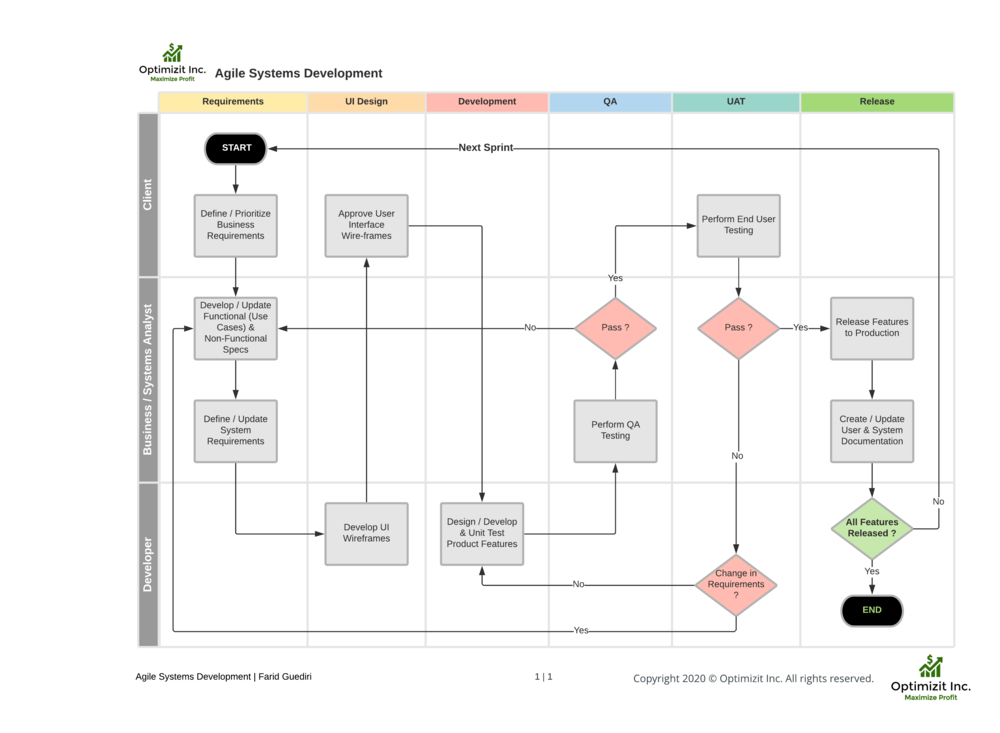
\includegraphics[width=1\textwidth]{imgs/BPM/sprint as bpm.png}
    \caption{Exemplos de um método ágil modelado como um BPM}
    \label{fig:bpm}
\end{figure}

Com isso, surgem os LIMS (Laboratory Information Management Systems) que, utilizando BPMs, conseguem organizar o fluxo de trabalho dentro de um laboratório para maior automação de processos e aumento da eficiência de cada etapa dentro de um determinado escopo \cite{Key2011}. Os LIMS nada mais são que softwares criados especificamente ou genericamente para um fluxo de trabalho específico.

A utilização de um LIMS traz grandes vantagens para laboratórios que o utilizam, como a automação de processos e coleta e armazenamento de dados \cite{Key2011}. Os LIMS usam de BPMs para abstrair atividades (uma ação dentro do BPM) que podem ser repetidas ou não, como em experimentos que devem ser refeitos ou atendimento a pacientes. 

Um BPM pode conter várias atividades que podem ou não depender uma das outras. No caso de um laboratório, realizar um experimento seria considerado uma atividade, calibração das máquinas seria outra atividade, obtenção de produtos também se transforma em outra atividade.

Para um fluxo de trabalho muito grande, temos uma profundidade grande nas atividades (como veremos na figura \ref{fig:centrareEstrutura}), ou seja, existe um ramo de atividades uma seguida da outra em sequência. Nós chamaremos isso de profundidade de atividades dentro do fluxo.

Caso uma atividade esteja muito profunda no ciclo do BPM (para chegar até ele, deve ser passado por muitas atividades anteriores), temos o problema de acesso desta atividade pelo usuário no LIMS, ou seja, muita informação (que podem ser desnecessárias) é mostrada ao usuário até que ele chegue à atividade esperada.

A proposta desse trabalho é alterar a visualização do BPM dentro do LIMS, dando mais facilidade para que o usuário acesse, preencha e complete suas tarefas com maior praticidade e agilidade dentro do espaço de trabalho, sem a necessidade de passar pelas atividades anteriores à desejada.

Também existe um problema de falta de compartilhamento de atividades entre BPMs, o que deixa o fluxo de trabalhos laboratoriais travado para um workflow em específico, já que uma atividade pode necessitar de informações de outras atividades (como um paciente que pode ter informações importantes junto a outros familiares também pacientes). Assim, o trabalho de implementar o compartilhamento de tais atividades entre diferentes fluxos de trabalho para que os dados sejam compartilhados entre setores ou até mesmo entre laboratórios está sendo feito, permitindo a unificação de BPMs com atividades em comum.

Testamos a implementação já existente da troca de ordem de atividades nos seguintes workflows: CENTRARE, um fluxo de trabalho para o Centro de Tratamento e Reabilitação de Fissura Labiopalatal e Deformidade Craniofacial do hospital da baleia, em belo horizonte, e o workflow BPL (Boas Práticas de Laboratório), que tem como finalidade registrar informações sobre os procedimentos usados no laboratório.
% \section{Materiais e Métodos} \label{methods}

% deve
% • ser elaborada de acordo com as especificidades da pesquisa realizada
% • de modo geral, este parte deve:
% a) descrever o tipo de pesquisa que foi realizada;
% b) narrar as etapas da pesquisa na ordem cronológica dos seus acontecimentos;
% c) anunciar os métodos, técnicas e instrumentos de coleta empregados, como também os critérios de seleção do universo e da amostra pesquisada;
% d) informar minuciosamente o delineamento experimental da pesquisa;
% e) descrever como se deu a coleta de dados e o tipo de coleta que foi realizada;

\subsection{Problemas}

\subsubsection{Acesso à informações}

Foi identificado um problema de acesso à certas atividades em um fluxo de trabalho com muitas repetições por parte de médicos em sistemas LIMS. Com isso, foi elaborado uma maneira de trocar a ordem dos BPMs para maior facilidade de acesso direto à atividade desejada sem a perda de informações.

Para isso, precisamos trocar a ordem do BPM sem perder os dados da atividade, já que a própria transição entre atividades pode significar algum tipo de informação por si só (exemplo: um experimento só deve ser realizado após um outro experimento)

BPMs podem ter múltiplas atividades iniciais e múltiplas atividades finais \cite{Dijkman2008}. Utilizando desse conceito, o workflow a ser alterado foi dividido em duas partes (figura \ref{fig:realWorkflow}): 

\begin{itemize}
    \item Um evento inicial que aponta para a atividade desejada pelo usuário
    \item Um evento inicial que aponta para a atividade inicial do workflow, preenchido até a atividade escolhida para ser a nova primeira atividade inicial
\end{itemize}

\begin{figure}
    \centering
    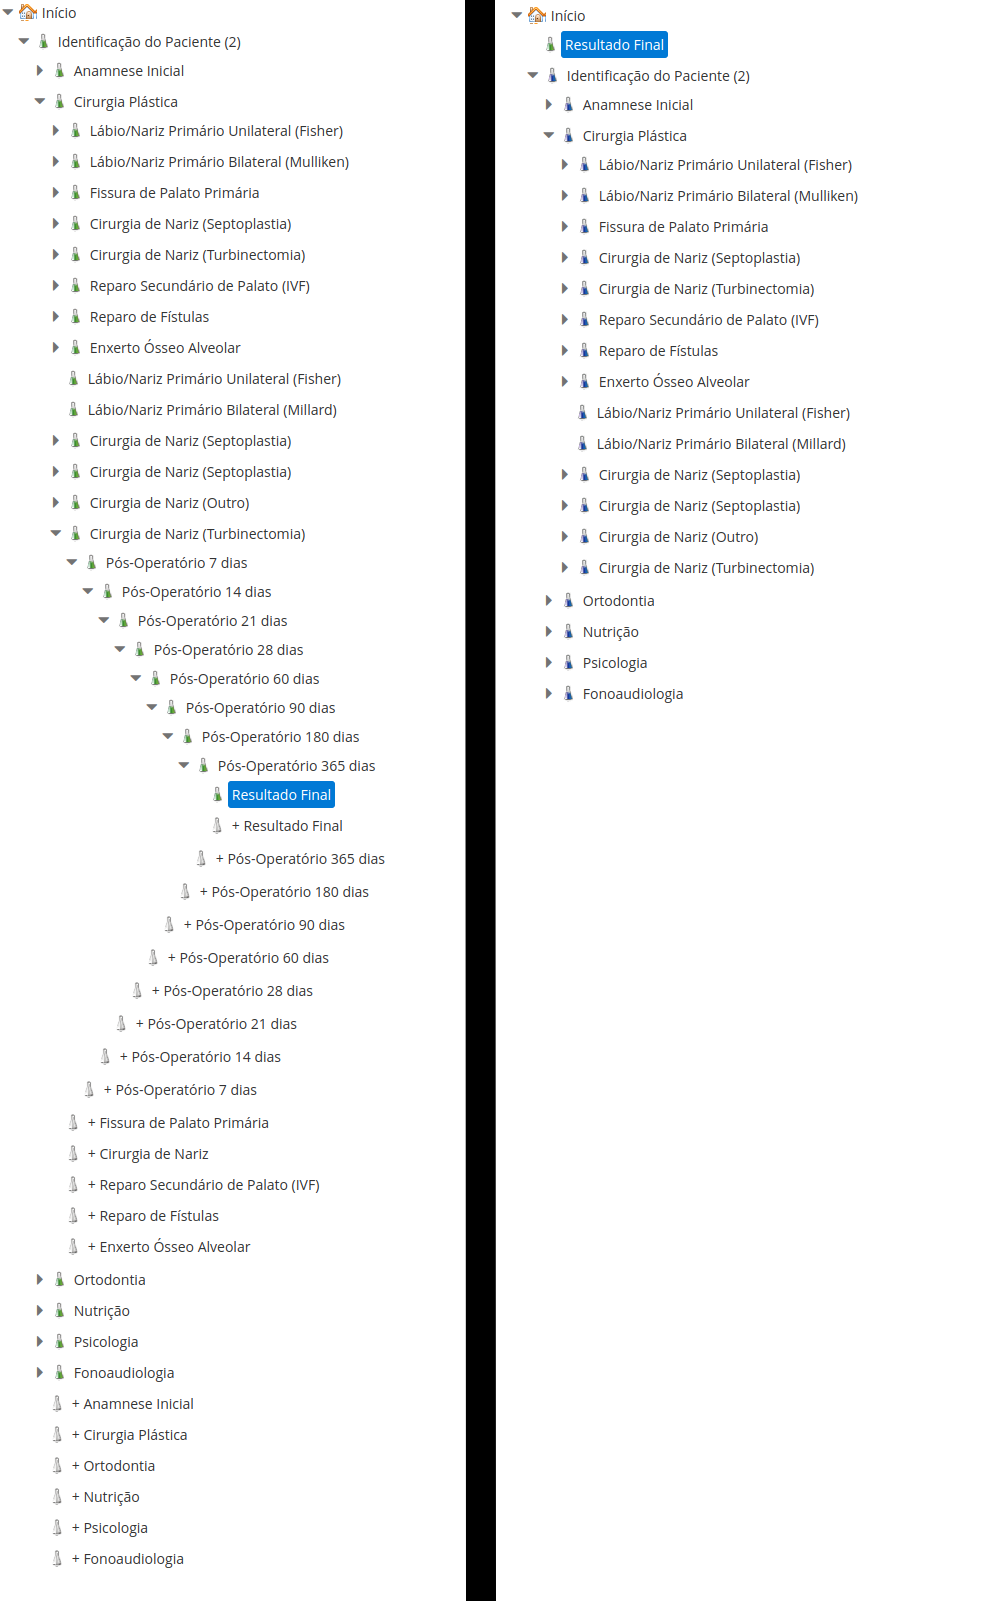
\includegraphics[width=10cm,height=15cm]{imgs/CENTRARE/arvoreNormalEAlterada.png}
    \caption{Workflow com árvore de atividades original à esquerda e workflow com árvore de atividades alterada à direita.}
    \label{fig:realWorkflow}
\end{figure}

Assim, ficam duas atividades iniciais: a primeira com a atividade que o usuário deseja preencher e continuar com seus trabalhos, e a segunda com o workflow original, contendo todas as informações necessárias para o preenchimento da atividade escolhida.

\subsection{Coleta dos dados Dados}

Foi utilizado o LIMS Flux, um LIMS generalizado que pode implementar fluxos de diversos laboratórios com uma interface gráfica presente dentro do próprio sistema \cite{Melo2010}. O Flux é uma ferramenta criada na linguagem Java, utilizando JavaServer Faces como framework de Front-end. O servidor utilizado para deploy é o Apache Tomcat.

Nele, utilizamos dados coletados de três workflows: O workflow BPL - Equipamentos, BPL - POP e o workflow CENTRARE. Os workflows BPL - Equipamentos e BPL - POP servem para controle de equipamentos e registro de informações sobre os procedimentos usados no laboratório, respectivamente, enquanto que o CENTRARE é um workflow para acompanhamento de pacientes com fissura de palato, desde o nascimento até os 20 anos, feito em conjunto com o hospital da baleia em Belo Horizonte.

Os workflows na ferramenta Flux seguem a notação de BPMs (BPMN - Business Process Model Notation) para representar os workflows implementados. Com isso, foi possível testar nesta ferramenta a troca de atividades iniciais e seu impacto nos trabalhos feitos pelo laboratório e fazer a prova de conceito sobre a alteração do fluxo de trabalho em BPMs.

Para o BPL (figura \ref{fig:bplEstrutura}), temos muitos usuários utilizando o mesmo workflow. Mas como o workflow é pouco profundo, com duas até no máximo cinco atividades de profundidade e com maior número de instâncias (ou seja, várias repetições da atividade inicial) ao invés de repetição de atividades dentro do workflow, temos que a centralização em algum atividade específica pode ajudar, mas não é muito necessária.

\begin{figure}
    \centering
    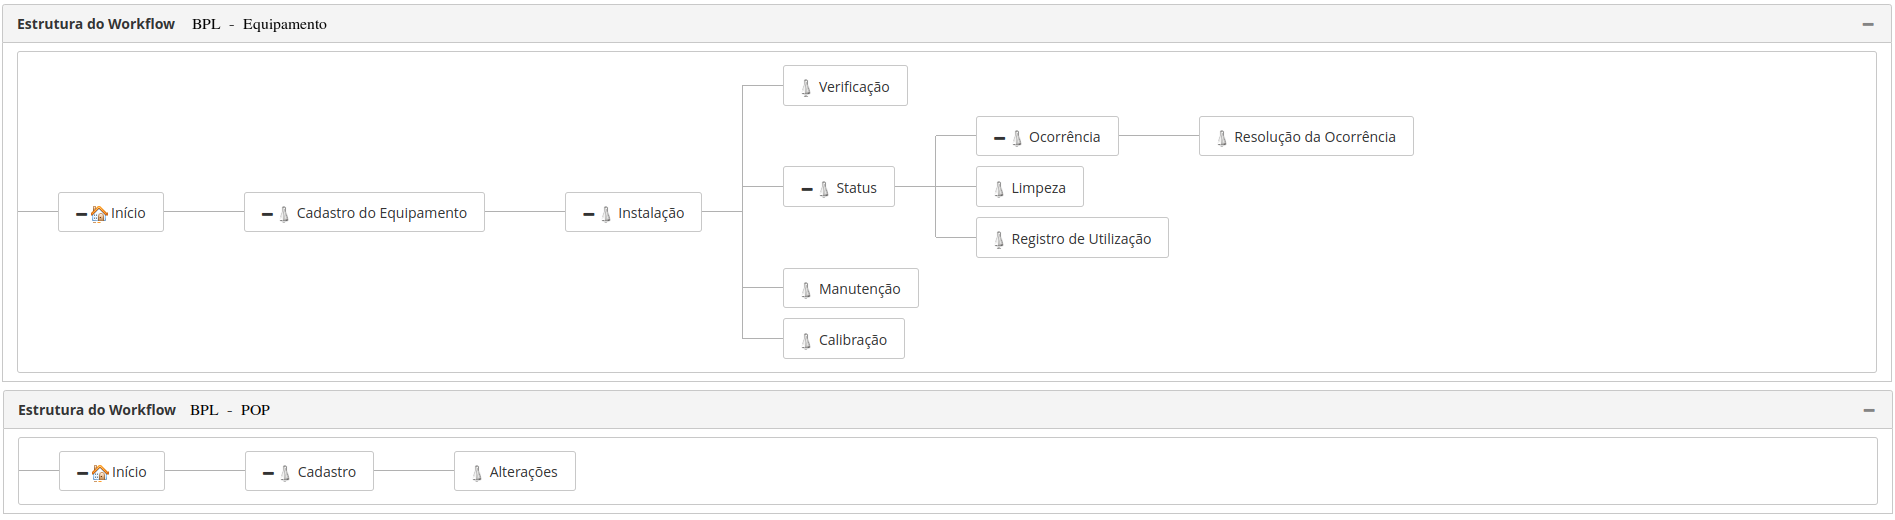
\includegraphics[width=1\textwidth]{imgs/BPL/estrutura.png}
    \caption{Estrutura dos workflows BPL - Equipamentos (Acima) e BPL - POP (Abaixo)}
    \label{fig:bplEstrutura}
\end{figure}

\subsection{Estrutura de workflows}

Para o CENTRARE (figura \ref{fig:centrareEstrutura}), temos muitos médicos que acompanham pacientes separadamente em vários setores de tratamento como cirurgia de palato, cirurgias odontológica, nutricionistas, psicólogos, fonoaudiólogos, entre muitos outros, e todas essas informações ficam em uma instância de um paciente em específico. Isso faz com que tenhamos muitas informações importantes apenas para pessoas específicas no fluxo de tratamento, com uma profundidade grande de atividades no fluxo de trabalho.

\begin{figure}
    \centering
    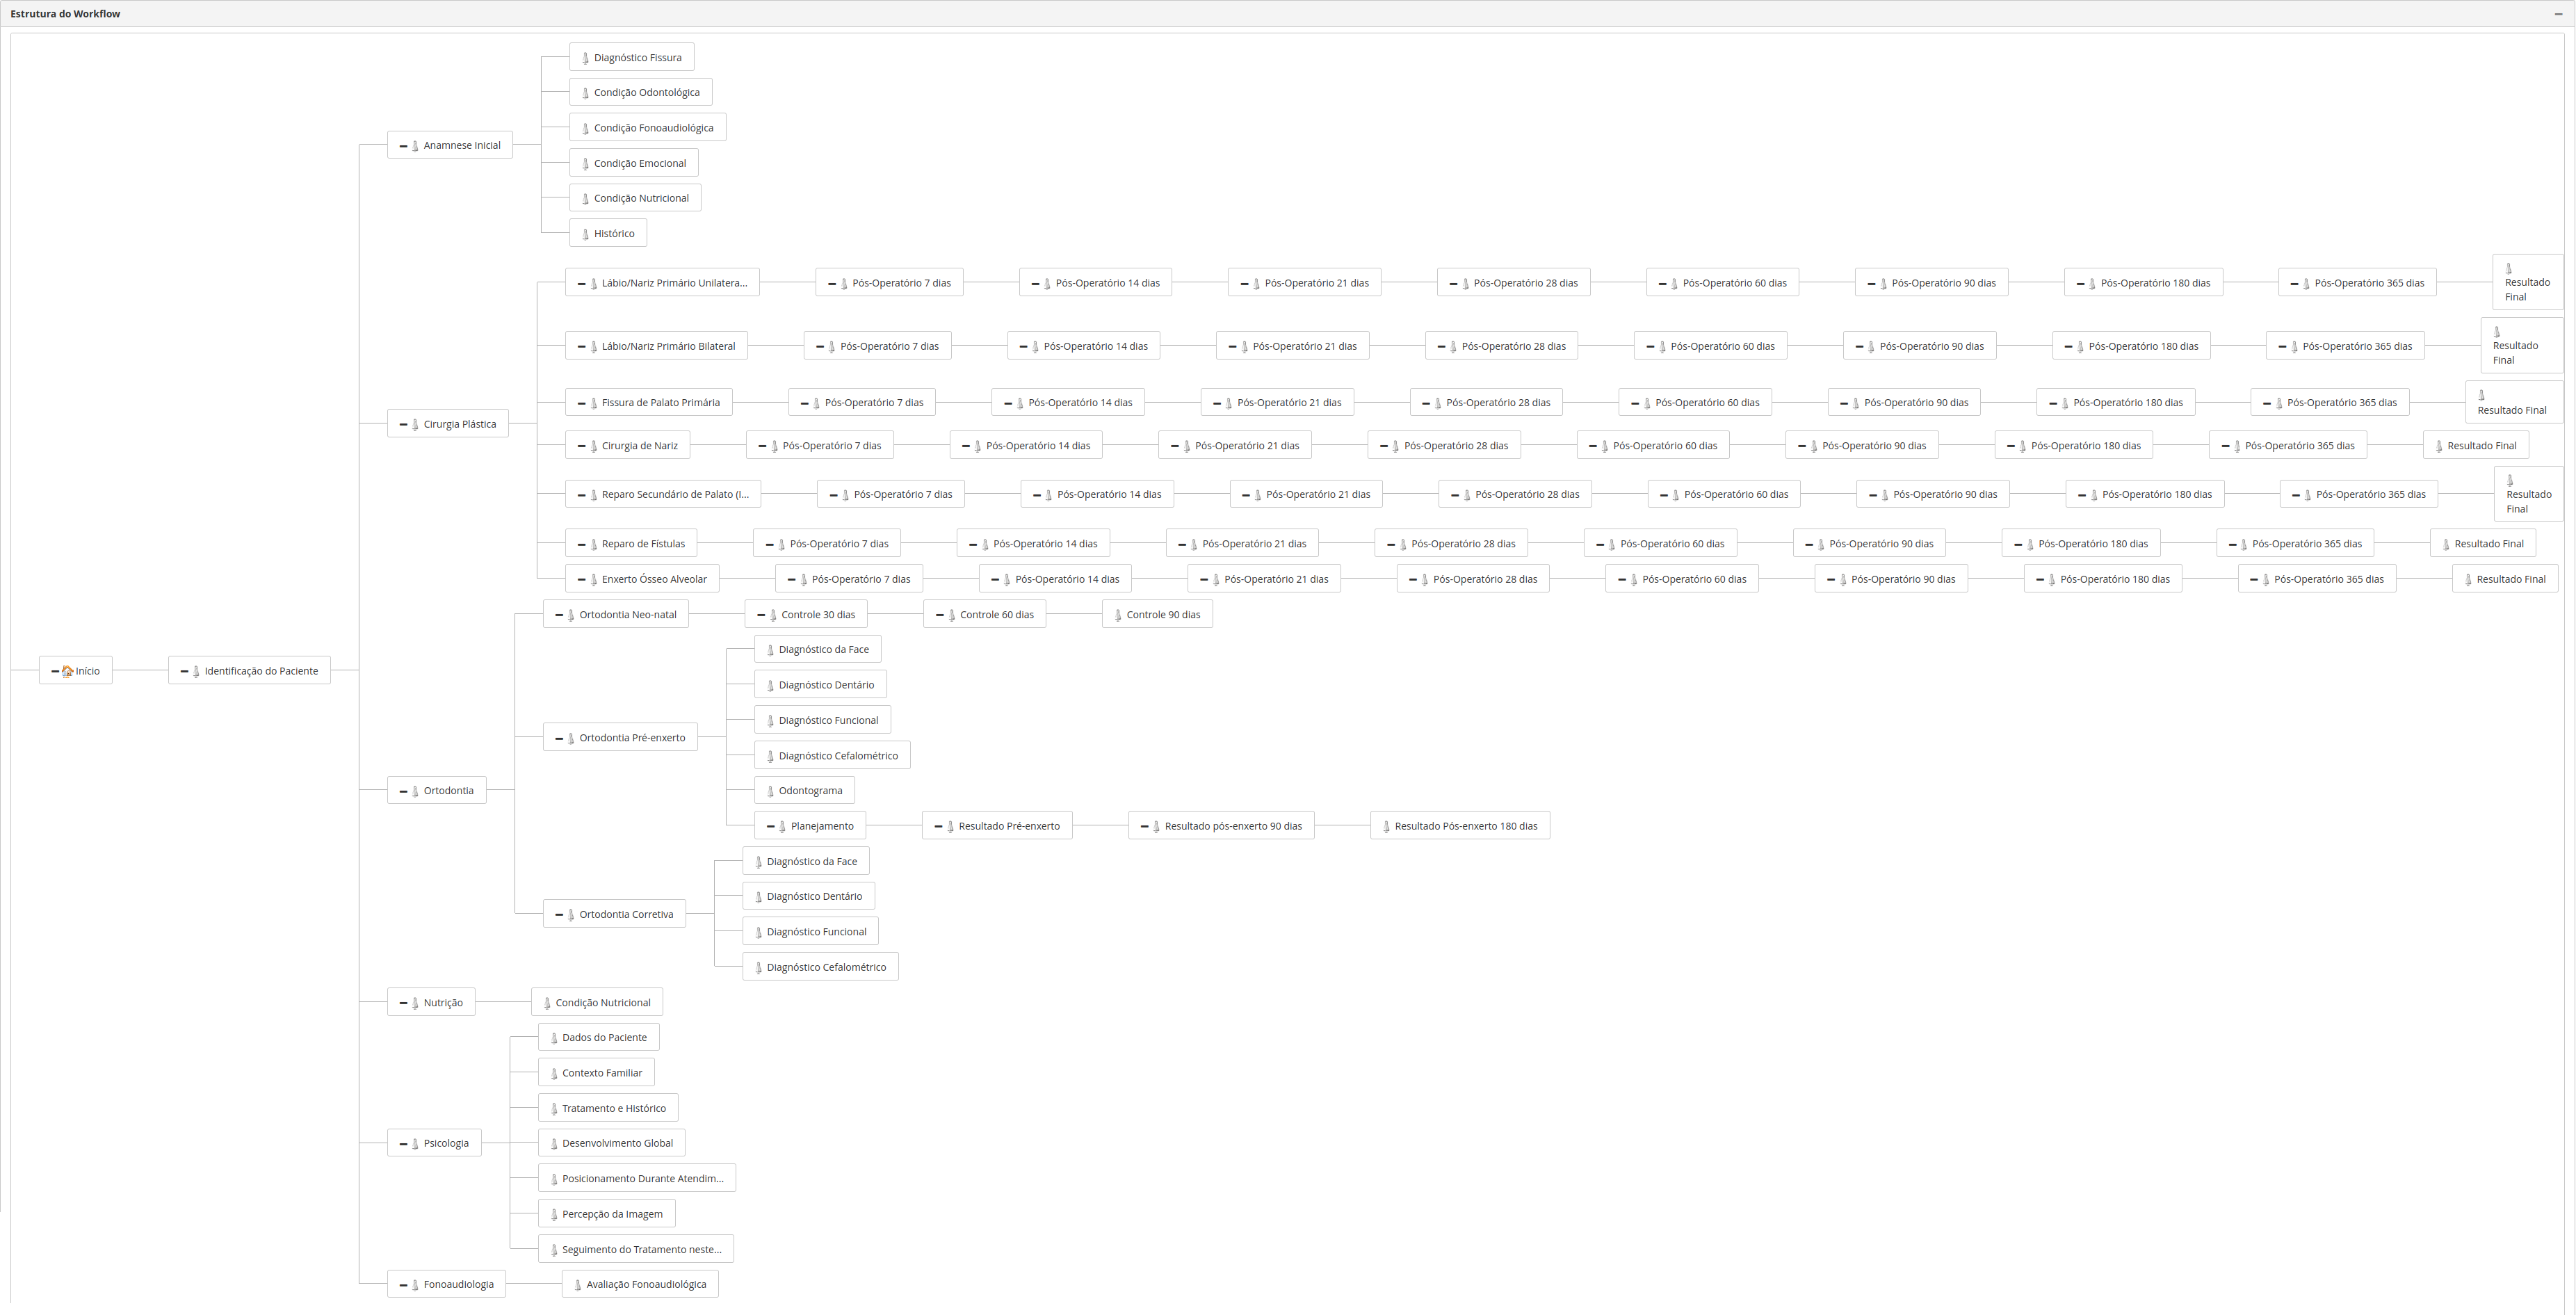
\includegraphics[width=1\textwidth]{imgs/CENTRARE/estrutura.png}
    \caption{Estrutura do workflow CENTRARE}
    \label{fig:centrareEstrutura}
\end{figure}

A centralização de atividades específicas é muito benéfica neste caso: Muitas pessoas trabalhando em partes do fluxo, mesmo que as atividades sejam dependentes de atividades anteriores, já que conseguimos "pular" atividades anteriores que podem não ser tão interessantes para a execução da atividade atual (exemplo: Um diagnóstico feito pelo ortodontista pode não ser interessante para o cardiologista) mas ainda assim obter informações necessárias com o segundo ramo de atividades criado.

Nos workflows BPL, temos dois fluxos que necessitam de compartilhamento de informações, já que um experimento não pode ser realizado se algum equipamento não for calibrado. Como não são as mesmas pessoas que trabalham no mesmo workflow (o técnico dos equipamentos não faz o experimento), com a implementação de BPMs atuais, não é possível que o cientista obtenha essa informação sem pesquisar no outro fluxo de trabalho para encontrar a informação requerida.

Com isso, o compartilhamento de atividades entre BPMs para obtenção de informações ajudaria os cientistas e técnicos a automatizar o envio de emails quando uma atividade se tornasse disponível após uma calibração, o compartilhamento de informações onde um cientista pode dar a informação que um equipamento necessita de reparos ou o técnico pode obter informações de quantos experimentos já foram feitos em um determinado período de tempo em alguma máquina.

Como exemplo de outros workflows que são melhorados com o compartilhamento de atividades são workflows de telemedicina, onde compartilhamento de informações entre pacientes e entre profissionais de saúde é de extrema importância. Também pode ser compartilhado informações administrativas do hospital, tendo informação de quais leitos estão disponíveis, quais produtos (como soros ou remédios) estão disponíveis para uso e quantos médicos estão disponíveis no momento para determinada função.

Também é importante ter o compartilhamento de mensagens entre workflows de biomedicina em laboratórios, em que o compartilhamento de informações entre experimentos ajuda tanto para armazenamento de produtos quanto para os resultados que são importantes para administradores, técnicos de equipamentos e também para outros cientista que estão realizando outros experimentos. Com o compartilhamento de atividades, o administrador do laboratório pode ver quantos experimentos foram realizados em determinada data, informar técnicos que determinado equipamento necessita de manutenção e fazer controle de estoque de itens necessários para o funcionamento correto do local.

\subsection{Implementação}

A implementação de centralização de atividades já foi realizada, começando em otimizações e preparação do sistema Flux. A implementação de compartilhamento de atividades entre workflows estão sendo realizadas e será finalizada até a defesa do mestrado.

Como este recurso requere muitas alterações para adaptação do LIMS Flux, além de várias iterações para chegarmos a uma implementação que faz sentido para o compartilhamento de atividades - como exemplo, existem workflows hospitalares que atividades compartilhadas entre médicos e administradores devem ser vistas apenas pelo administrador, ao invés de todas as atividades administrativas ficarem disponíveis para todos os médicos - este recurso está sendo implementado no momento e ficará pronto até a defesa do mestrado.
% \section{Resultados} \label{results}

% deve
% • apresentar uma descrição detalhada dos dados coletados de modo que aqueles que estiverem lendo o trabalho possam ter a exata dimensão do que foi apreendido na pesquisa.
% • os dados podem ser apresentados em forma de tabelas, quadros, gráficos e outras figuras ilustrativas como fluxos, esquemas, etc., que devem ser inseridos o mais próximo possível do trecho do texto no qual se inicia a descrição dos principais resultados apresentados na figura.

Com a alteração do fluxo de trabalho para ser iniciado em uma atividade escolhida pelo usuários, podemos visualizar na figura \ref{fig:changedWorkflow} o novo fluxo de trabalho, indicando o corte do workflow na atividade selecionada, transformando a atividade selecionada em um novo ponto de inicio e adicionando uma nova atividade inicial no fluxo de trabalho. Assim, caso o usuário queira acesso à atividades anteriores para obter informações que podem ser necessárias para a nova atividade inicial ou para futuras atividades, ele pode visualizar estas informações acessando o flux dividido, enquanto que para acessar próximas atividades e poder criar novas atividades, o usuário pode seguir no novo fluxo principal.

No caso do workflow CENTRARE, podemos ver pela figura \ref{fig:changedInstance} que, ao selecionarmos uma nova atividade inicial, temos mais funcionalidades na hora de selecionar qual atividade realmente queremos acessar (com a disponibilização de busca de atributos da atividade, busca por nome da atividade ou data de criação), além de diminuir consideravelmente o número de cliques que o usuário deve fazer para acessar a atividade (figura \ref{fig:changedWorkflow}).

\begin{figure}
    \centering
    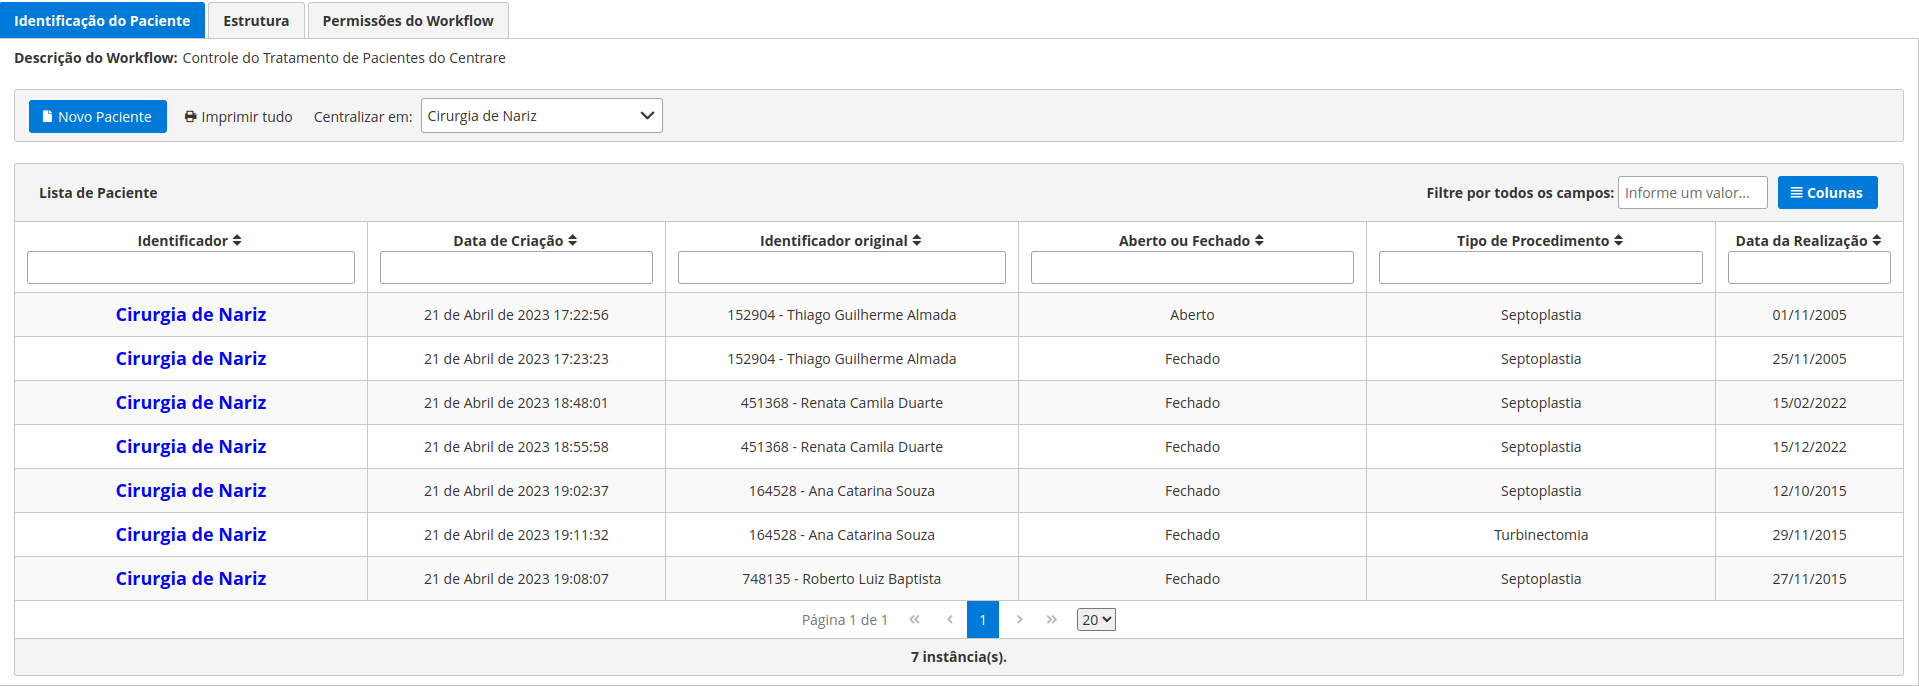
\includegraphics[width=1\textwidth]{imgs/CENTRARE/instanciaAlterada.png}
    \caption{Lista de instâncias do workflow CENTRARE, centralizado na atividade "Cirurgia de nariz"}
    \label{fig:changedInstance}
\end{figure}

Com a modificação da árvore de atividades, temos também a divisão de informações que limpa a tela para o usuário, retirando parte das informações parcialmente desnecessárias que o usuário teria que navegar para chegar na atividade que será preenchida no momento.

Como uma das maiores reclamações em softwares de teleatendimento e de softwares de manejamento de laboratórios é uma experiência de usuário confusa, sem levar em conta o contexto do usuário na ferramenta nem do que o usuário necessita dentro da ferramenta para obter um resultado em suas atividades, o remanejo de atividades em um BPM facilita a utilização da ferramenta e, com isso, aumenta a eficiência da utilização do software.

No caso do workflow BPL, temos que os benefícios não são muito aparentes pelo tamanho do workflow e também pelo número de instâncias que são criadas (disponibilizando informações para preenchimento com sua atividade inicial original). Isso faz com que a consulta de atividades se torne mais fácil e não existem muitas informações que podem ficar omitidas atrás de muitas atividades.

No caso do workflow CENTRARE, a centralização de atividades foi muito benéfica, já que o workflow tem uma profundidade considerável e o número de pessoas que trabalham nesse workflow também é grande. Com a centralização, encontrar atividades que são interessantes para o usuário em determinado momento é uma questão de selecionar a atividade a ser selecionada e fazer a busca dos dados pelos atributos da atividade escolhida.

Como a identificação original do workflow é pelo paciente, que pode ter uma ou mais cirurgias, para que o médico encontre uma cirurgia específica, ele apenas centraliza o workflow na atividade da cirurgia desejada e procura pelos atributos desejados, sem que precise lembrar de qual paciente foi a cirurgia.

Para o compartilhamento de informações, o CENTRARE poderia ser dividido em vários workflows separados para cada tipo de funcionário (nutricionista, psicologo, fonoaudiologo) e, com o compartilhamento de informações entre workflows, um novo workflow poderia ser montado com esta divisão em mente e haver uma maior separação de informações entre os profissionais, mantendo apenas informações importantes disponíveis para cada um.

No BPL, como já dito, temos o compartilhamento de mensagens entre técnicos e cientistas para obter informações de equipamentos e experimentos realizados, além dos gerentes de laboratório tendo as duas informações condensadas em um só lugar.

Há também, para futuros BPMs implementados, o controle de estoque facilitado com troca de informações (como um laboratório que compartilha racks com outro laboratório e necessita da informação de disponibilidade, mantendo sempre essa informação atualizada entre laboratórios)
% \input{sections/conclusao}

\section{Introdução}

\subsection{Sistemas de informações modernos}

% Big data 
% Grande número de informações

Nos últimos anos, temos observado um aumento exponencial na quantidade de dados gerados em todo o mundo, provenientes de diversas fontes como redes sociais, dispositivos móveis, sensores IoT e transações financeiras.
Esses dados são muito importantes para empresas e organizações de todos os setores, pois fornecem informações valiosas sobre o comportamento do consumidor, as tendências do mercado, desempenho dos negócios e até mesmo dados internos como utilização de recursos dentro da empresa.

No entanto, a gestão desses dados pode ser um desafio, pois eles estão dispersos em diversos locais, podendo ter sido salvos em diferentes formatos. Além disso, é essencial garantir a segurança e a privacidade dessas informações, especialmente quando se trata de dados confidenciais de clientes, pois podem ser dados sensíveis que não podem ser disponibilizados para o público.

A análise de dados também é uma parte crítica desse processo, pois permite que as empresas compreendam e usem seus dados para tomar decisões de negócios mais informadas. Com a análise de dados, as empresas podem identificar tendências e padrões em seus dados, permitindo que elas otimizem seus processos e melhorem a experiência do cliente.

Para lidar com esses desafios, os sistemas de controle de acesso, coleta e análise de dados tornaram-se cada vez mais importantes. Esses sistemas permitem que as empresas gerenciem seus dados com segurança e eficiência, garantindo que apenas pessoas autorizadas possam acessá-los e que as informações sejam coletadas e armazenadas de maneira adequada.

Para áreas de telemedicina, laboratorial e biomédica, este tipo de sistema é essencial para o armazenamento, processamento e segurança das informações coletadas, se integrando com o ambiente onde foi implementado para aumentar a eficiência dos trabalhos e tornar possível a análise de todos os dados coletados nos trabalhos feitos.

Esses sistemas permitem que pesquisadores, médicos e profissionais da saúde gerenciem e analisem grandes quantidades de dados de pacientes e estudos clínicos com mais eficiência e segurança, diminuindo a incidência de erros que podem ocorrer~\cite{Sun2021LaboratoryEfficiency}. Estes sistemas são chamados de sistemas biomédicos.

\subsection{Sistemas biomédicos}

Sistemas biomédicos trazem muitos benefícios à área biomédica, como a melhoria de segurança, garantindo acesso aos dados apenas para pessoas autorizadas, aumento de eficiência por disponibilizar a coleta de dados automatizada quando o sistema está integrados com equipamentos, reduz erros de entrada de usuários por garantir que os dados estejam corretamente formatados e também melhoram a gestão de recursos devido a análise de dados que podem ajudar, por exemplo, instituições médicas, que utilizam esta tecnologia para garantir que os recursos estejam sendo usados de maneira eficiente e econômica.

Para isso, é fundamental que se tenha uma maneira eficiente de gerenciar e armazenar essas informações, disponibilizando a integração entre variados tipos de equipamento como sensores de temperatura, monitores cardíacos e medidores de pressão arterial. Este tipo de funcionalidade é altamente procurada por laboratórios, surgiram sistemas especializados para que a integração laboratorial seja feita de maneira rápida e simples. Assim surgiram os sistemas de gerenciamento de informações de laboratório, ou LIMS.

% Coleta de informações

% Tempo gasto ao salvar dados~\cite{Sinsky2016}

% Armazenamento e organização

% Segurança

% Gestão de laboratórios é extremamente necessária no mundo tecnológico em que vivemos hoje. Aumento de eficiência, automação de processos, gestão de tempo e funcionários são algumas das funcionalidades que são procuradas atualmente em diversos laboratórios~\cite{sun2021laboratory}. Para esse tipo de gestão, é necessário algum meio de formalizar fluxos de trabalhos para que sejam de fácil entendimento e reproduzíveis. 

% Para isso, muitas soluções foram pensadas para atacar este problema, tanto na parte de armazenamento de dados quanto em segurança de dados \R. Como exemplos de soluções feitas para armazenamento de dados laboratoriais, temos \R, \R e \R.
\subsection{LIMS}

% O que são LIMS

LIMS (Laboratory Information Management System) é um tipo de sistema de gerenciamento de informações de laboratório que permite o gerenciamento e controle de todas as informações e processos de laboratório em um único sistema integrado. Ele ajuda os laboratórios a automatizar e gerenciar tarefas complexas como coleta, armazenamento e análise de dados, gerenciamento de amostras e rastreabilidade, gerenciamento de estoque e inventário, além de garantir a conformidade regulatória.

% Porque são relevantes de acordo com os pontos anteriores

A utilização do LIMS oferece diversos benefícios, como maior eficiência operacional, redução de erros manuais, melhoria da qualidade dos dados, automação de fluxos de trabalho e melhoria da colaboração e compartilhamento de informações~\cite{Key2011LIMS:Systems}. O LIMS também ajuda na rastreabilidade de amostras e resultados, permitindo que os usuários identifiquem facilmente a origem dos dados e possam rastrear as informações em caso de necessidade~\cite{Cagindi2004ImportanceFactories}.

% Como são utilizados no setores: Médicos, Laboratoriais

Nos setores médicos, esses sistemas são usados para gerenciar registros eletrônicos de pacientes, permitindo que os médicos e profissionais de saúde acessem e atualizem informações em tempo real, o que ajuda na tomada de decisões clínicas mais precisas e rápidas. Esses sistemas também são usados para gerenciar e rastrear amostras de pacientes, bem como para gerenciar o estoque de medicamentos e suprimentos médicos.

Nos setores laboratoriais, os softwares LIMS são usados para gerenciar e rastrear amostras de pacientes, bem como para gerenciar o fluxo de trabalho e o inventário de reagentes e equipamentos. Esses sistemas ajudam a garantir a rastreabilidade e a integridade das amostras, a melhoria da qualidade dos dados e a conformidade com as regulamentações.

Além disso, os LIMS são utilizados em laboratórios de pesquisa para gerenciar grandes volumes de dados e informações de experimentos, garantindo a precisão, segurança e a integridade dos dados. Esses sistemas também ajudam na colaboração entre os membros da equipe de pesquisa, facilitando o compartilhamento de informações e resultados.

LIMS podem ser feito de diversas maneiras para integrar as atividades de um laboratório ao software, e uma dessas maneiras pode ser utilizando BPMs.

% Como podem ser utilizados em tudo

% A utilização de um LIMS traz grandes vantagens para laboratórios que o utilizam, como a automação de processos e coleta e armazenamento de dados~\cite{Key2011}. Os LIMS baseados em BPMs usam a modelagem em BPM para abstrair atividades (uma ação dentro do BPM) que podem ser repetidas ou não, como em experimentos que devem ser refeitos ou atendimento a pacientes. 
\subsection{Problemas com LIMS hoje}

% Introdução ao problema com LIMS hoje

Os LIMS hoje, mesmo com todos os benefícios como automatização de tarefas, redução de erros manuais, aumento da produtividade e rastreamento de dados, ainda sofre de grandes problemas que, muitas vezes, limitam a sua implementação dentro de ambientes médicos e laboratoriais.

Os problemas vão desde a personalização de interface até o custo de implementação, manutenção e suporte dentro da organização~\cite{Avery2000ProductGuide., CommmonAstrix}.
Os LIMS não são tão personalizáveis porque, em grande parte dos casos, eles são projetados para atender a um conjunto específico de requisitos regulatórios e padrões de indústria, além de envolverem a integração de muitos componentes diferentes como banco de dados, interface do usuário e sistemas de instrumentação que podem dificultar a personalização do mesmo.

Outro problema que dificulta a personalização de um LIMS é a necessidade de manter a validação e a conformidade regulatória, já que cada personalização do sistema deve passar por uma validação vigorosa para garantir a qualidade e integridade dos dados não foram comprometidas.
Com isso, há um aumento da complexidade de implementação e um aumento do custo, já que um programa desses passa a ser parte do dia a dia do trabalho na empresa e pode sofrer alterações para manter o fluxo de trabalhos atualizado.

% Problema na visualização de atividades

% Problema na aceleração de acesso à informação

A falta de personalização de um LIMS pode levar a problemas adicionais relacionados à visualização e acesso à informação. Quando um sistema LIMS não é personalizado para atender às necessidades específicas do laboratório, as informações podem ser apresentadas de maneira desorganizada, o que dificulta o acesso e a visualização dos dados relevantes. Por exemplo, um laboratório que realiza vários tipos de testes pode ter dificuldades para visualizar informações específicas de um teste em particular, se o sistema LIMS não estiver configurado adequadamente para exibir essas informações de maneira clara e organizada.

% Porque isso deve ser melhorado?

Além disso, a falta de personalização pode tornar a navegação pelo sistema LIMS mais difícil, o que pode levar a erros ou omissões no registro e interpretação dos dados. Se os usuários não conseguirem acessar rapidamente as informações de que precisam, eles podem inadvertidamente inserir dados incorretos ou perder informações críticas. Isso pode levar a erros na análise dos resultados dos testes e na tomada de decisões clínicas.

Portanto, a personalização adequada de um sistema LIMS é essencial para garantir que as informações sejam apresentadas de maneira clara e organizada e que os usuários possam acessá-las facilmente. A interface do usuário deve ser projetada para ser intuitiva e fácil de usar, permitindo que os usuários naveguem facilmente pelas informações relevantes. Além disso, o sistema deve ser capaz de exibir informações personalizadas para diferentes usuários ou grupos de usuários, de modo que cada pessoa possa acessar as informações relevantes para suas tarefas específicas.

% Quem liga pra esse problema?

Como exemplo, um LIMS com interface dinâmica implementado na área hospitalar para assistir na execução de atividades entre a equipe médica e a equipe laboratorial pode beneficiar tanto médicos quanto outros profissionais de saúde que trabalham com laboratórios pois terão acesso a informações revelantes que ajudarão a orientar o tratamento de seus pacientes de maneira mais rápida e eficiente.
\subsection{Business Process Models}

% O que é BPM

O BPM (Business Process Models) é uma abordagem sistemática para a gestão de processos de negócios que envolve o mapeamento, análise e melhoria dos processos para melhorar a eficiência, qualidade e eficácia. Ele busca identificar as etapas envolvidas em um processo, as pessoas e sistemas envolvidos, bem como os principais indicadores de desempenho para monitorar e melhorar os resultados.

% Comparação da utilizade dos sistemas e do BPM

Tanto os sistemas de controle de acesso, coleta e análise de dados quanto o BPM têm como objetivo a automação e gerenciamento de processos complexos em uma organização. Ambos buscam melhorar a eficiência operacional, reduzir erros e aumentar a qualidade dos resultados.

% De volta ao BPM

BPMs modelam uma série de etapas sequenciais que precisam ser realizadas para se completar uma tarefa ou processo específico, conhecidos como fluxo de trabalho. Eles são utilizados para definir como processos serão realizados, definindo objetivos dentro de uma organização~\cite{Alves2014UnderstandingOrganizations}. Eles podem ser utilizados para abstrair fluxos de trabalho existentes e criar novos fluxos com maior facilidade, podendo ser construídos seguindo uma das várias notação de BPMs, como a BPMN (Business Process Model and Notation)~\cite{Dijkman2008SemanticsBPMN}.

% BPMs (Business Process Models) são modelos de fluxos de trabalho utilizados para definir como processos serão realizados, definindo objetivos dentro de uma organização~\cite{Alves2014}. Eles podem ser utilizados para abstrair fluxos de trabalho existentes e criar novos fluxos com maior facilidade, podendo ser construídos seguindo a notação de BPMs, a BPMN (Business Process Model and Notation)~\cite{Dijkman2008}.

% Para que podem ser utilizados

BPMs são utilizados em uma ampla variedade de organizações, independente do setor ou do tipo de atividades. Sua aplicação ajuda as organizações a gerenciar e melhorar os seus processos de negócio, documentando como ele é feito e que passos devem ser seguidos para reprodução do mesmo \R. Assim, os trabalhos podem ser melhor divididos entre os integrantes de uma equipe e pode-se encontrar falhas ou oportunidades de melhoria dentro de um processo.

% Onde são utilizados

% Exemplos de utilização

No setor de saúde, temos a utilização de BPM pelas instituições para gerenciar processos clínicos como atendimento ao paciente, gestão de agendamento, faturamento e gestão de registros médicos. Além disso, pedidos de exame e cadastro de amostras podem ser modelados para maior facilidade de compartilhamento de informações entre funcionários.

% Introdução ao próximo capítulo LIMS e BPMS

BPMs são geralmente ilustrados com diagramas de fluxo, demonstrando um Fluxo de trabalho (workflow) com uma sequência de atividades e decisões tomadas no projeto, como pode ser visto no exemplo de método ágil modelado em BPM na figura~\ref{fig:bpm}.

A implementação de BPM dentro de uma organização ajuda a identificar pontos de melhoria no processo já instaurado, podendo aumentar a colaboração entre departamentos e garantir que o fluxo de trabalho seja feito de maneira eficiente e, principalmente, consistentemente \R.
Além disso, os BPMs podem ajudar a monitoria e automatizar certos processos dentro de uma empresa, já que todos estarão bem documentados. \R

\begin{figure}
    \centering
    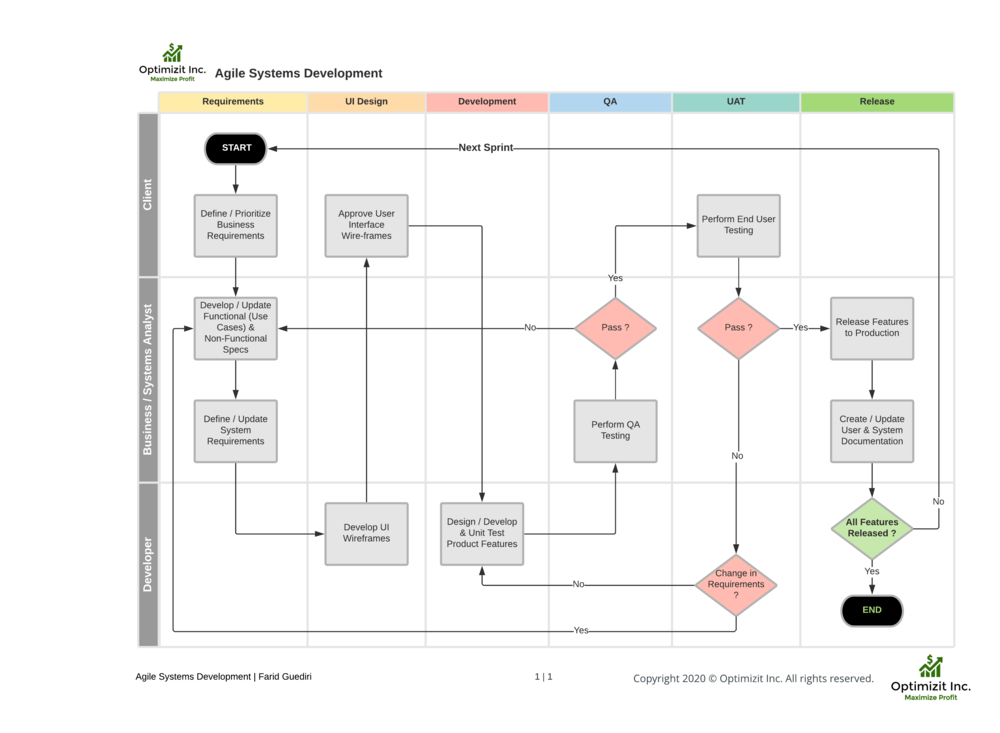
\includegraphics[width=1\textwidth]{imgs/BPM/sprint as bpm.png}
    \caption{Exemplos de um método ágil modelado como um BPM}
    \label{fig:bpm}
\end{figure}

BPMs podem ser utilizados com LIMS, para organizar o fluxo de trabalho dentro de um laboratório. Com isto, obtém-se uma maior automação de processos e um aumento da eficiência de cada etapa dentro de um determinado escopo~\cite{Key2011LIMS:Systems}.

É importante que um LIMS esteja integrado com todos os passos do BPM modelado, especialmente em laboratórios e indústrias farmacêuticas, químicas e de biotecnologia, ajudando a melhorar a eficiência operacional, aumentando a precisão dos resultados e reduzindo erros com a automatização de tarefas repetitivas e da validação dos dados a serem colocados no sistema.

% É muito importante que um LIMS esteja integrado com partes do processo que são utilizadas para armazenar dados, como coleta e processamento de amostras em um ambiente laboratorial, pesquisa de dados dentro do programa para dados médicos, entre muitos outros, para que a sua implementação seja justificada e que o aumento de eficiência seja bem mensurado.

Para isso, os LIMS devem ser personalizáveis para que possam ser integrados com outros sistemas que podem ser utilizados dentro da organização para garantir a compatibilidade e a interoperabilidade entre diferentes sistemas utilizados.
\subsection{LIMS baseados em BPM}

% Utilização de LIMS junto a BPMS

LIMS baseados em BPMs juntam a modelagem de fluxos de trabalho com a utilização do BPM e a gestão de dados em um LIMS, ajudando a melhorar a eficiência e qualidade dos processos de laboratório e permitindo que os usuários configurem, gerenciem e monitorem os processos de forma mais eficiente. Isso é feito através da automação de fluxos de trabalho, permitindo que as tarefas sejam atribuídas aos usuários corretos, no momento certo e com a quantidade certa de informações~\cite{LIMS-BPMSLaboratory, LIMS-BPMSLaboratoryb}.

Além disso, o uso de BPM em um LIMS permite a integração de diferentes sistemas e aplicativos, facilitando a comunicação entre as equipes e melhorando a colaboração, já que todo o processo de negócio das equipes estará modelada dentro do LIMS. A padronização dos processos também ajuda a garantir a qualidade e precisão dos dados gerados pelo laboratório~\cite{LIMS-BPMSLaboratory, LIMS-BPMSLaboratoryb}.

% Exemplos de uso ultimamente

\subsubsection{Vantagens de LIMS baseados em BPM}

Os BPMs trazem melhorias significativas com sua utilização em um LIMS, como a padronização de processos que serão executados, reduzindo a variabilidades nos resultados e melhorando a confiabilidade das análises, além de facilitar a automatização de tarefas repetitivas e padronizadas, o que diminui ainda mais os erros e aumentam a produtividade. \R

Com a definição do fluxo de negócios implementada em um LIMS, é possível também fazer a otimização deste processo, já que o BPM permite a identificação de gargalos e pontos de melhoria nos processos de laboratório, permitindo uma melhoria contínua. \R

Um LIMS implementado em laboratórios de saúde pode ser utilizado para gerenciamento de coleta, processamento e análise de amostras de pacientes. Quando um BPM está implementado neste mesmo LIMS, há a definição dos processos envolvidos na realização dos mesmos por meio de diagrama de fluxos, facilitando sua otimização e colaboração entre as equipes de laboratório e outros departamentos. \R

Com a definição do processo e gerenciamento dos dados pelo LIMS, diminui-se a quantidade de erros que podem acontecer na entrada de dados pelos usuários do software, já que se pode ter uma integração grande com o software de armazenamento de dados diretamente com uma máquina que processa amostras médicas, por exemplo.

Também há a maior facilidade de seguir regulamentações. Os laboratórios são regulamentados por várias agências reguladoras, como a FDA (Food and Drug Administration), ANVISA (Agência Nacional de Vigilância Sanitária) e ISO (International Organization for Standardization). Essas agências estabelecem requisitos rigorosos para garantir a qualidade e segurança dos produtos e serviços fornecidos pelos laboratórios.

A utilização de um LIMS que implementa BPM aumenta a rastreabilidade de amostras desde o momento que são recebidas até o momento em que são descartadas, melhora o gerenciamento de documentos como procedimentos operacionais padrão (SOPs) e também servem para auditoria dos processos e validação dos resultados por salvarem todas as informações dentro dos seus bancos de dados, garantindo que eles sejam precisos e confiáveis e atendam aos requisitos regulatórios.

% Qual a vantagem e desvantagem com LIMS que não utilizam BPMs

\subsubsection{Desvantagens de LIMS baseados em BPM}

Algumas das desvantagens de uma implementação de LIMS com BPM juntos é o preço de implementação, complexidade para o usuário, personalização do BPM para o LIMS e falta de flexibilidade a depender da implementação do software.

O preço vem da complexidade de implementação das duas tarefas: tanto do LIMS quanto do BPM \R. Com a complexidade de implementação, vem também a complexidade para os usuários entenderem sua utilização em uma interface intuitiva \R.

A integração entre BPM e LIMS também pode gerar muitas dificuldades no quesito de personalização de interface e implementação de um BPM que seja muito complexo para o LIMS que esteja tentando implementá-lo. Caso este seja o caso, o LIMS deve ser alterado para que este processo possa ser implementado corretamente. Com isso, há uma maior dificuldade de flexibilidade do software, já que alguns softwares não suportam que sejam feitas muitas alterações para que um BPM complexo possa ser corretamente modelado dentro do sistema.
\subsection{O que pode ser feito}

% Qual LIMS foi utilizado

Este trabalho apresenta uma nova maneira de execução de fluxo de trabalho de BPMs dentro de um LIMS para que a personalização da interface do usuário seja integrada com BPMs. Para isso, foi utilizado o LIMS Flux (mais explicado na seção~\ref{sec:flux}) para implementação de workflows dinâmicos.

Workflows dinâmicos permitem que o usuário centralize sua visão em uma atividade central desejada, sendo particularmente útil em organizações que possuem workflows complexos que contém muitas atividades, envolvendo várias etapas para ser executado.

% Quem isso afeta e porque é importante?

A funcionalidade de centralização de atividade dentro de um workflow pode ser utilizada pelos usuários para selecionar a atividade desejada para obter dados requeridos de maneira mais rápida, atendendo às necessidades específicas daquele usuário de maneira pontual. Isso permite que cada pessoa se concentre nas atividades que são mais relevantes para suas tarefas no momento da utilização do software, personalizando seu uso.

Quando o usuário seleciona uma atividade a ser centralizada, o LIMS altera a ordem do BPM para que o usuário tenha uma melhor visualização do workflow, transformando a atividade selecionada na atividade inicial do BPM.

Atividades anteriores à selecionada ficam disponíveis para obtenção de dados que podem ser necessários para execução da atividade centralizada, sendo disponíveis com mudanças na interface para identificar que a atividade é anterior à selecionada.

% Solução quanto ao acesso de informações resolvida com o trabalho

Para que esta implementação fosse mais poderosa no sistema, também foi implementado a junção de diferentes BPMs em um único BPM com múltiplas atividades iniciais que podem ser compartilhadas entre eles. Assim, quando um usuário faz mais de uma função em um laboratório, ele pode acessar os diferentes fluxos de trabalho da mesma interface, até mesmo centralizando as atividades dos diferentes workflows com a funcionalidade explicada anteriormente.

Esta implementação ajuda a unificar as informações dentro do sistema dentro de uma única interface, facilitando o acesso às informações e aumentando a eficiência da utilização do LIMS, além de possibilitar o compartilhamento de atividades entre execuções de um processo de negócios.

% Como foi feito

% Relação com BPM

% Utilização no Flux
\section{Sistemas de coleta de dados}

\subsection{Importância}

% Importância de sistemas biomédicos hoje

O grande volume de dados gerados e utilizados por aplicações e como analisá-los é tema de várias pesquisas, sejam elas por corporações ou por pesquisas acadêmicas \R. Principalmente na área biomédica, temos a geração de enormes quantidades de dados com a evolução das tecnologias de sequenciamento genético \cite{luoJ2016}.

As áreas de telemedicina também estão sofrendo avanços enormes nos últimos anos com a vinda da pandemia do SarsCov2, o Covid19 \cite{bakhtiar2020, kronenfeld2021, GatesB.Colbert2020UtilityEra}, e com isso também houve o aumento exorbitante da geração de dados no campo médico para que houvesse um atendimento mais rápido e melhorado dos pacientes \cite{MohdKhanapiAbdGhani2018PDFData, Coakley2015TransformingAnalytics}.

Essa quantidade de dados gerado deve ser armazenada, analisada e ter proteção contra acessos não autorizados. O software que obtiver essa quantidade de dados tem como responsabilidade assegurar todos os pontos anteriores, além de facilitar o acesso dos dados aos usuários por meio de interfaces facilitadoras.

Existem inúmeras soluções criadas para uso profissional, além de um grande número de pesquisas para tratar da crescente quantidade de dados gerados tanto por laboratórios quanto por sistemas de telemedicina \cite{Mangrulkar2022AutomaticTechniques}.

Essas soluções são chamadas de Laboratory information management system (LIMS), e já existem para uso pessoal ou de corporações, como o Bika \cite{Goodblatt2006FosteringProcess}, MetaLIMS \cite{Heinle2017MetaLIMSLabs}, Labvantage \cite{Smallmon2017BiobankingSilos}, Flux \cite{Melo2010SIGLa:Laboratories}, e suas funcionalidades serão explicados na seção \ref{sec:lims-exemplo}
% Quantidade de dados sendo gerados pela área médica e laboratorial

% Soluções existentes no mercado hoje

% Introdução aos LIMS
\subsection{LIMS}

% O que são (de novo)

Laboratory information management system (LIMS), ou sistema laboratorial de manejamento de informação são softwares criados para gestão de dados, processos, máquinas e pessoas de forma segura e muitas vezes automatizada~\cite{Stafford1998LIMS:Technology}.

% Onde podem ser utilizados

LIMS podem ser utilizados em qualquer sistema que necessita de coleta de dados, automação e integração de pessoas e máquinas para obtenção de resultados consistentes e para manter a segurança de tais dados~\cite{Sun2021LaboratoryEfficiency, TowardsXplore}.

Um dos exemplos deste tipo de cenário é na área de telemedicina, que, com a vinda da pandemia do SarsCov2 no fim de 2019, sofreu um aumento significativo de sua utilização com mais e mais pacientes surgindo e com lockdowns acontecendo, fazendo com que pessoas ficassem em casa e não pudessem fazer visitas médicas presenciais~\cite{kronenfeld2021, bakhtiar2020, GatesB.Colbert2020UtilityEra}.

Isso também levou ao grande aumento de dados sendo guardados por sistemas. Em muitos hospitais, ainda é utilizado sistemas antigos, guardando dados escritos a mão em grandes salas utilizadas apenas para armazenamento de dados de pacientes~\cite{2021TacklingMachine}. Este tipo de sistema, utilizado na pandemia, diminui muito a eficiência das equipes e não pode ser escalonado para grandes quantidades de dados.

% Exemplos de utilização, tanto em áreas médicas ou laboratoriais

O próprio governo brasileiro expandiu a utilização de softwares no sistema único de saúde (SUS), aumentando o projeto de centralização dos dados de pacientes por todo o país para que todos fossem armazenados em um banco que todos os médicos tivessem acesso para melhoria na eficiência de processos e unificação de hospitais~\cite{Araujo2021DesafiosCovid-19}, utilizando o e-SUS, com enfase na "estratégia para reestruturar as informações da Atenção Primária em nível nacional"~\cite{E-SUSAPS}.

Para a área laboratorial, temos diversos exemplos de utilização para automação de processos e experimentos, além de aumento no nível de segurança de dados e facilitação no gerenciamento e análise dos mesmos, sendo necessário pela grande quantidade de dados que um laboratório pode gerar com seus experimentos, além do dever de seguir rigorosas regras de regulamentação~\cite{Holzmuller-Laue2014ImprovedAutomation, Holzmuller-Laue2013Model-drivenLaboratories}.

% Quais categorias de pessoas são as melhores para utilizar o software (Manager, developer, médico, paciente...)

É importante que o LIMS esteja integrado com toda a atividade de onde está sendo utilizado para que aumente a eficiência e automação das atividades dentro do ambiente implementado. Isso inclui a utilização pelos funcionários, sendo o LIMS moldado para todo tipo de funcionário na companhia.

Existem inúmeras maneiras de se construir um LIMS, sendo uma delas a modelagem dos trabalhos da organização em etapas sequenciais, cada uma com seus próprios requisitos de entrada e saída, seguindo uma estrutura de fluxo de trabalhos, podendo ser modelado com o modelo de Business Process Management (BPM)~\cite{Holzmuller-Laue2014ImprovedAutomation}.

BPM é uma metodologia de modelar trabalhos e processos que gera atividades representando fluxos de trabalho que são necessários para chegar a um objetivo dentro de uma organização. Com a modelagem do BPM, chegamos a uma arquitetura de processos que pode ser dividida de maneira a aumentar a eficacia de um grupo de pessoas no trabalho modelado~\cite{Hammer2015WhatManagement}.

% Utilização de BPMs no LIMS

Ao utilizar o BPM com LIMS, podemos utilizar o BPMN, ou Business Process Management Notation, uma notação que é padronizada~\cite{Chinosi2012BPMN:Standard} e pode ser utilizada juntamente a um LIMS para modelar os processos e já poder integrar o fluxo de trabalho diretamente ao software de coleta de dados e automatização de processos~\cite{Holzmuller-Laue2013AAutomation}.

% Beneficios de BPMs ( https://proceso.pro/en/blog/pros-and-cons-of-business-process-management-bpm/ )

A utilização de BPMs em LIMS ajuda na produtividade dos usuários, já que o sistema pode definir e automatiza partes do processo, reduzindo assim a quantidade de erros no processo por restringir as partes críticas das atividades seguindo as políticas do laboratório.
Com isso, temos também a redução de micro manejamento dos gerentes da empresa, por ter um controle sobre os dados maior com medidas de segurança e por todos os funcionários seguirem o mesmo protocolo de preenchimento de dados e acatamento de resoluções~\cite{BenefitsManagement}.

% Maleficios de BPMs ( https://proceso.pro/en/blog/pros-and-cons-of-business-process-management-bpm/ )

Seguindo os princípios dos benefícios do BPM, as desvantagens de sua integração podem ser a falta de comunicação entre pessoas para seguir as regras da empresa caso os processos sejam modelados de maneira a não permitir a comunicação entre usuários do software, dificuldade em inovações caso a modelagem seja muito restritiva, não permitindo pensamentos criativos dentro da empresa.

Estas desvantagens podem aparecer principalmente quando há uma abordagem inadequada ou excessivamente rígida na implementação da gestão de processos, e não necessariamente serão sempre um problema na organização que o implementa.

Para isto, é importante que tenham pessoas experientes com BPMs para implementação do mesmo dentro da organização, que demonstra mais um malefício dos BPMs: O custo elevado e a complexidade de implementação.

Para implementar corretamente um BPM, deve-se ter um alinhamento estratégico com os objetivos da organização, levando em consideração todas as partes que a compõem como, no caso de um laboratório, gerência, técnicos de laboratório, cientistas e estudantes.

% Beneficios de LIMS ( https://genemod.net/blog/lims-the-good-the-bad-and-the-ugly )

% Eficiencia, acuracia e produtividade

Os benefícios da utilização de um LIMS em um ambiente laboratorial vem do aumento da eficiência dos cientistas, técnicos, gerência e comunicação externa entre laboratórios vinda da integração do software com as partes necessárias para gravação e obtenção de dados. Sendo assim, um LIMS seguro pode fornecer todos os dados em uma tela rápida para a gerência e, caso um cientista vir a utilizar do software, ter outra tela mais relevante disponibilizando apenas as informações necessárias para aquele individuo, aumentando assim sua produtividade.

% Maleficios de LIMS  ( https://genemod.net/blog/lims-the-good-the-bad-and-the-ugly )

Os problemas que podem vir da implementação de um LIMS é que, se mal implementado, a interface pode ser não intuitiva, de forma a diminuir a produtividade dos envolvidos. Caso este LIMS não integre com as partes laboratoriais, ele pode se tornar uma dificuldade a mais no dia a dia do usuário, tendo que repetir dados em locais diferentes pela falta de automação, fazendo com que a acurácia também caia - erros de entrada de dados no programa podem ocorrer.

% Porque são importantes

% Como guardam os dados

Os dados de um LIMS precisam ser guardados em bancos de dados seguros e apenas liberar o acesso a esses dados para pessoas autorizadas, então é necessário que tenha um modelo de segurança de acesso integrado para que isso seja possível. esta necessidade existe pois os dados que estão nestes LIMS, muitas vezes, são dados sensíveis e que devem ter ser acessíveis apenas pelas pessoas autorizadas.

% Como lidam com segurança dos dados

Desta forma, é implementada uma hierarquia de usuários para que cada classe de usuário (Gerente, cientista, técnico...) tenha diferentes tipos de acesso aos dados. Assim, é possível gerenciar quais usuários tem acesso a quais tipos de dados dentro do sistema, mantendo um nível de segurança dinâmico para cada usuário diferente do software.

% Benefícios de sua utilização

% Malefícios de sua utilização

% Arquitetura: Como são construídos (Seguindo que base)

% Como há a disponibilização de dados aos usuários

% Problemas atuais

% Beneficios que BPM trazem no LIMS

% Problemas que BPMs trazem no LIMS
\subsection{Exemplos de sistemas utilizando BPM} \label{sec:lims-exemplo}

Nesta seção iremos falar sobre alguns LIMS que são conhecidos e citaremos algumas das suas capacidades para integração de um fluxo de trabalho dentro deles.

\subsubsection{Bika}

Bika é um LIMS gratuito que pode ser utilizado por qualquer organização. Além de ser um LIMS de graça, ele tem integração com vários equipamento biomédicos, mas ainda faltam interações entre equipamentos essenciais que fazem dele um LIMS menos poderoso por não conseguir se integrar com o fluxo de trabalho do laboratório de maneira generalizada \cite{Ademuyiwa2018DevelopmentBiobanking}.

O Bika permite que organizações configurem suas próprias práticas de laboratório, fluxos de trabalho, modelos de dados e relatórios de saída. O sistema é baseado em um modelo de informações flexível que pode ser adaptado às necessidades específicas de um laboratório.

Algumas das principais funcionalidades que se destacam são as de gerenciamento de amostras, gerenciamento de ensaios, gerenciamento de resultados e gerenciamento de clientes dentro do mesmo software.

A integração de equipamentos laboratoriais deve ser programada individualmente para cada equipamento pelos desenvolvedores do sistema, diminuindo a integração do software dentro da organização.

Além disso, a interface implementada para uma organização segue tópicos de preenchimento, não seguindo um fluxo de trabalho como um BPM modelado. Assim, seguir um passo a passo nesta plataforma fica com uma maior propensão ao erro, já que a plataforma deixa que o usuário execute qualquer tipo de atividade a qualquer momento.

\subsubsection{MetaLIMS}

O MetaLIMS é um sistema de gerenciamento de informações de laboratório (LIMS) que foi projetado para atender as necessidades de laboratórios de pesquisa e desenvolvimento (P\&D) em ciências da vida, química e materiais. Ele é desenvolvido pela MetaSystems, uma empresa que oferece soluções para laboratórios de genômica e citogenômica.

O sistema permite que os usuários registrem informações sobre amostras, experimentos, resultados, protocolos e instrumentos de laboratório em um único local centralizado. Ele também permite que os usuários rastreiem o status das amostras em tempo real, gerenciem tarefas e atribuam recursos, além de oferecer recursos de geração de relatórios e visualização de dados.

MetaLIMS utiliza conceitos de BPM (Business Process Management) para gerenciar os fluxos de trabalho e processos de laboratório. Ele permite que os usuários definam e gerenciem fluxos de trabalho personalizados para cada tipo de experimento ou análise, desde a solicitação da amostra até a geração de relatórios finais, definindo etapas sequenciais, atividades paralelas e condições de entrada e saída.

\subsubsection{Labvantage}

O Labvantage LIMS é um sistema de gerenciamento de informações de laboratório (LIMS) desenvolvido pela LabVantage Solutions, uma empresa de software que oferece soluções para laboratórios em diferentes setores. O sistema é projetado para atender às necessidades de laboratórios de diferentes tamanhos e complexidades em diversas indústrias, incluindo farmacêutica, biotecnologia, alimentos e bebidas, ambiental e química.

O LabVantage permite que os usuários configurem fluxos de trabalho de forma flexível, definindo etapas sequenciais, atividades paralelas e condições de entrada e saída por meio de definição do fluxo de trabalho utilizando BPM. Isso ajuda a garantir que todos os experimentos e análises sigam um processo padronizado e controlado, aumentando a qualidade e a confiabilidade dos dados gerados.

\subsubsection{Flux}

O LIMS Flux é um sistema de gerenciamento de informações de laboratório (LIMS) que permite que laboratórios gerenciem e rastreiem seus processos e dados de amostras. Ele será melhor explicado na seção \ref{sec:flux}

% Exemplo 1: MetaLIMS

% Exemplo 2: Labvantage

% Exemplo 3: Thermofisher
\section{LIMS baseados em workflows}

% O que é o Flux

O LIMS Flux é um sistema de gerenciamento de informações de laboratório (LIMS) que permite que laboratórios gerenciem e rastreiem seus processos e dados de amostras. O LIMS Flux é um software baseado em nuvem que pode ser acessado de qualquer lugar, a qualquer momento, através de um navegador da web.

O sistema é altamente configurável e pode ser personalizado para atender às necessidades específicas de cada laboratório. Ele é projetado para ajudar laboratórios a gerenciar fluxos de trabalho, desde o registro de amostras até a geração de relatórios finais.

O Flux utiliza o conceito de BPM na construção de seus workflows, definindo cada parte do fluxo de trabalho como atividades e como atributos as informações dentro de cada atividade. Com isso, pode-se construir qualquer tipo de workflow dentro do Flux, podendo abstrair BPMs para serem implementados.

Com o treinamento necessário e o conhecimento técnico de modelagem de BPMs, um administrador laboratorial pode utilizá-lo para criar um workflow seguindo o BPM modelado para a organização, personalizando o fluxo de trabalho de maneira a se integrar com o laboratório.

Ele pode ser considerado um meta LIMS: O software pode ser utilizado para criação de workflows (fluxos de trabalho) com atividades e atributos que seguem os padrões de um laboratório ou telemedicina, conseguindo automatizar a entrada de informações da atividade e integrar com o restante do laboratório independente de outros softwares utilizados.

A integração de outros softwares é uma capacidade importante que permite que diferentes aplicativos e sistemas funcionem juntos, trocando informações de forma automática para melhorar a eficiência do LIMS. No caso do Flux, ele atinge essa funcionalidade com a funcionalidade de executar qualquer tipo de programa em qualquer linguagem por meio de plugins dentro do workflow criado.
Sendo assim, o Flux pode ser integrado com todo o laboratório, não sendo necessário que algum administrador do software implemente alguma iteração e disponibilize para os usuários.

% Porque o Flux foi utilizado

\subsection{Seleção do LIMS}

O Flux foi utilizado pela facilidade na modelagem de workflows variados utilizando BPM. Tendo em mente os objetivos deste trabalho, o Flux foi modificado para atender às demandas para resolução dos mesmos, como alteração da interface a depender do usuário que está utilizando do software, apresentando informações mais rapidamente para os usuários, diminuindo o tempo de busca dentro do programa e também a troca de informações entre diferentes BPMs, unificando a modelagem de diferentes tipos de workflows em um grande BPM com diferentes atividades iniciais.

% Como o Flux utiliza Business Process Model

Com a utilização de BPMs de maneira modular feito no Flux, há uma maior flexibilidade na modelagem dos processos dentro do software, diminuindo os custos de desenvolvimento de software já que qualquer pessoa que tem o conhecimento do próprio software e de construção de BPMs consegue desenvolver um fluxo de trabalho de um modelo de negócios.

Isso diminui (mas não elimina) alguns dos problemas que envolvem LIMS que implementam BPMs como o custo elevado pela complexidade de desenvolvimento do programa, pois ainda necessita de pessoas que saibam modelar os processos mas não necessariamente que sejam desenvolvedores de software.

% Como o Flux revela o problema de todos os LIMS com BPM

Com o Flux, construímos BPMs complexos para serem implementados no software, demonstrando a necessidade de melhorias na obtenção de dados para agilizar o trabalho dos usuários. Os BPMs complexos que foram utilizados são utilizados hoje por organizações que utilizam o Flux como ponto central nos trabalhos feitos.

BPMs, sendo apenas uma maneira de descrever fluxos de trabalho e modelagem de processos, não disponibilizam nenhuma forma de seleção de dados, ficando a dever do LIMS de implementar algum tipo de recurso para disponibilização de informações aos usuários.

Quando o fluxo de trabalho é muito grande, tomamos tempo do usuário, fazendo-o procurar dentro do fluxo de trabalho, em meio a inúmeras informações disponíveis, a informação que ele deve encontrar. Isso faz com que o usuário perca tempo em forma de inúmeros cliques dentro de uma interface que muitas vezes não é intuitiva~\cite{OvationIncNeeded:LIMS}.

Com múltiplas pessoas tendo diferentes funções dentro do mesmo workflow, é muito improvável que todas elas estejam fazendo a mesma função e necessitando das mesmas informações. A interface, então, deve ser alterada para que cada usuário tenha uma visão diferente quando está utilizando o LIMS para que, com uma experiência personalizada, haja uma diminuição do tempo de procura das informações buscadas.

Para a telemedicina, isso é de suma importância pois os médicos, que podem se tornar usuários de um LIMS, não gostam de diminuir a eficiência dos seus trabalhos aprendendo uma ferramenta nova e modelos de trabalho novos sendo que o modelo existente para armazenamento de dados já funciona para eles, então o LIMS deve ser intuitivo, personalizável e disponibilizar as informações necessárias com a menor resistência possível para o usuário.
\subsection{Atividades profundas}

% Definição de atividades profundas

Quando uma empresa modela seu processo de negócios em um BPM, é possível que existam muitos passos para completá-lo. Cada passo ou etapa no processo é chamado de atividade e, quando existem muitas atividades em sequência, chamamos de atividades profundas dentro de um processo.

Atividades profundas são aquelas que, a partir do início do fluxo de trabalhos, exigem um grande número de atividades intermediarias até que elas fiquem disponíveis, sendo necessário executar cada atividade anterior para alcançá-la.

% Problema em grandes workflows

Workflows complexos tendem a ter uma profundidade grande, que torna difícil a busca e a inserção de novos dados por usuários que o utilizam. Grandes workflows também podem ter múltiplos usuários em passos diferentes dentro do workflow, tendo diferentes objetivos de execução.

As atividades profundas surgem frequentemente quando um ambientes de negócios envolve muitos processos complexos, como na indústria de manufatura, setor de serviços financeiros ou em empresas com cadeias de suprimentos complexas. Essas atividades podem ajudar a garantir que todos os processos sejam executados de maneira consistente e eficiente, e que os objetivos sejam alcançados de forma efetiva, mas aumentam a profundidade do workflow consideravelmente, como podemos ver no workflow complexo do CENTRARE na figura~\ref{fig:centrareEstrutura}.

\begin{figure}
    \centering
    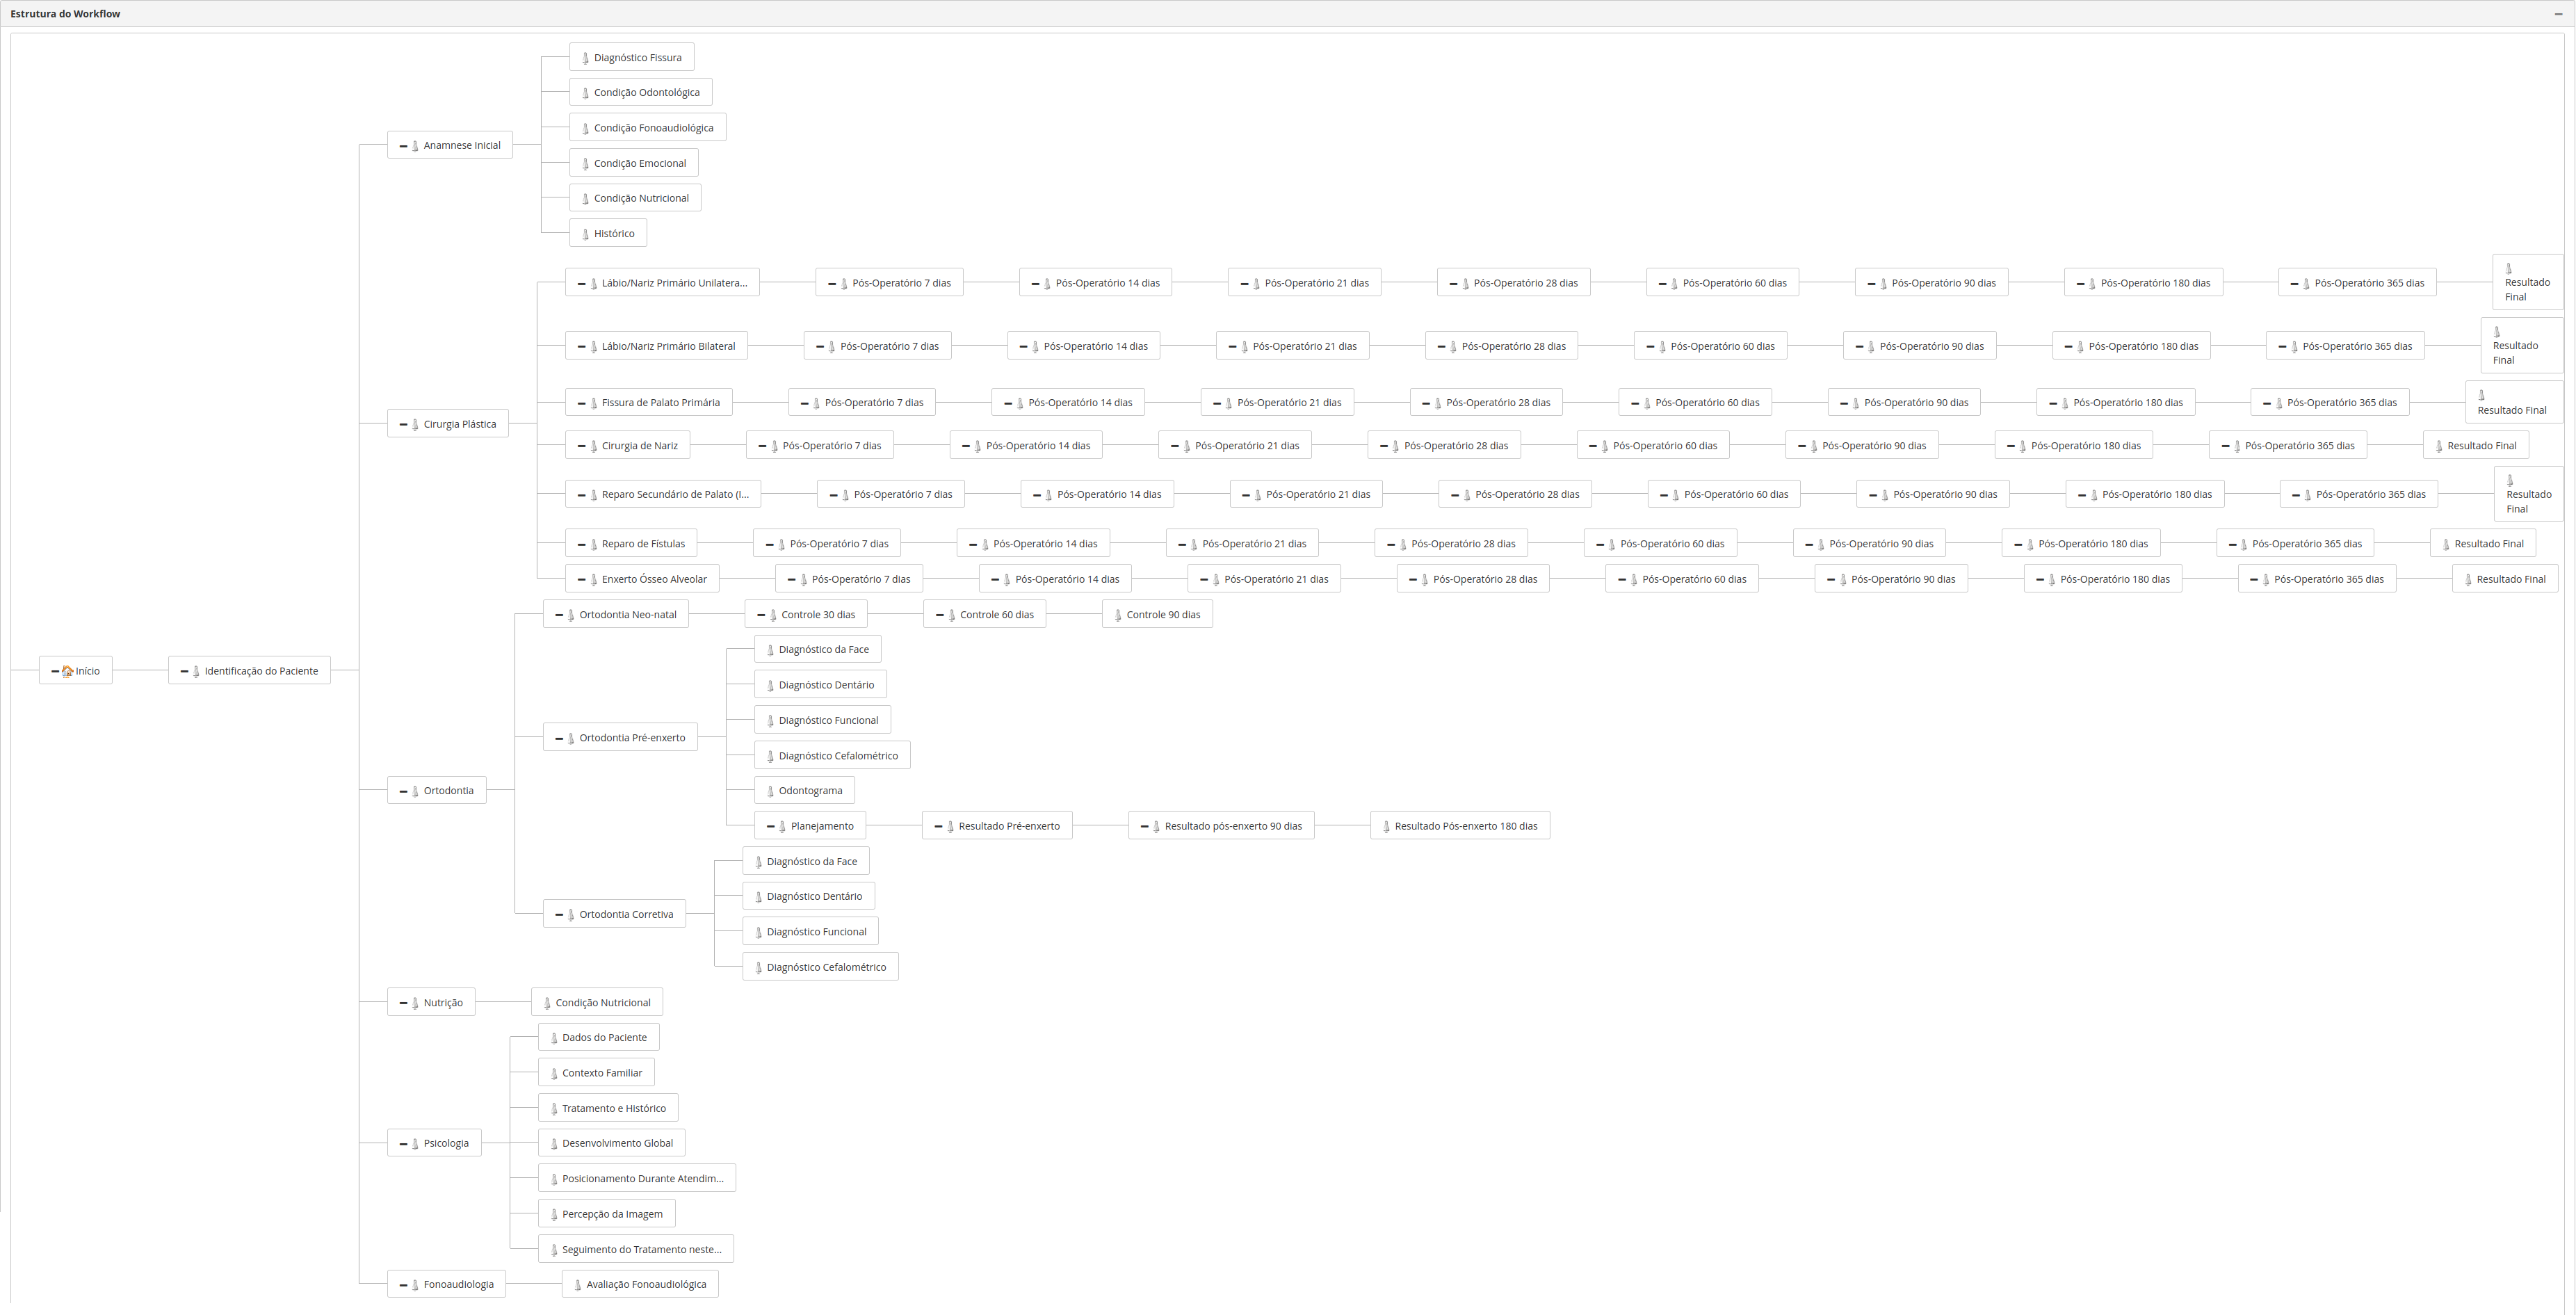
\includegraphics[width=1\textwidth]{imgs/CENTRARE/estrutura.png}
    \caption{Estrutura do workflow CENTRARE. Podemos verificar a quantidade de atividades em cada retângulo da estrutura em árvore, tendo um profundidade máxima de 12 atividades.}
    \label{fig:centrareEstrutura}
\end{figure}

% Porque isso é um problema

Essas atividades profundas podem virar um problema quando implementadas em um LIMS: Encontrar informações de maneira rápida e concisa pode não ser possível a depender das possibilidades de personalização de interface do LIMS, diminuindo a eficiência do trabalho dos funcionários que utilizam o software.

% Como isso se relaciona com Big Data

% Isso tem relação com a crescendo busca pela automatização de digitalização dos dados. Existem hoje informações sendo enviadas automaticamente para um sistema de coleta de dados por smart devices, como relógios ou "smart bands" que coletam dados de diversos tipos como dados cardiológicos, saturação de oxigênio, exercícios feitos pelo usuário, e isso aumenta a necessidade de softwares que coletam e armazenam dados com segurança.

% Este tipo de informações, por exemplo, pode ser utilizado em um sistema de telemedicina para coletar dados dos seus pacientes automaticamente, mandando notificações para o médico responsável pelo paciente caso algum dado precise de sua atenção.

A agregação, tratamento e disponibilização destes dados tanto para os usuários que o utilizam quanto para a empresa que os coletam é de grande importância para o desenvolvimento de soluções em aplicativos para saúde de usuários e também disponibilização de informações relacionadas com o estilo de vida das pessoas.

% Como isso se relaciona com a utilização com o médico

Muitas organizações que começam a implantação de um sistema LIMS para utilização de seus funcionários encontram uma grande resistência à adoção de novas tecnologias, especialmente se estiverem acostumados a trabalhar com processos manuais ou sistemas legados~\cite{2018CommonAstrix}. Essa resistência pode existir por alguns motivos como a complexidade do treinamento para sua utilização, a rapidez nos processos dentro do software e aversão à troca de sistemas já implantados pelo sistema novo.

Isso demonstra que a necessidade de uma interface intuitiva, rápida e eficaz para os usuários chave de um LIMS é de muita importância para sua implementação. Para que isso ocorra dentro de um workflow grande com atividades profundas é uma grande dificuldade, já que as informações dentro do programa devem ser todas mostradas para demonstrar um contexto (histórico hospitalar, por exemplo) que vai ser utilizado para completar a atividade atual, sem que isso interfira na utilização do software.

% Como isso se relaciona com a utilização de várias áreas

Como um exemplo de utilização de um LIMS em áreas laboratoriais, a disponibilização de informações para os funcionários, seja cientistas, seja engenheiros, seja gerentes de projeto, devem estar disponibilizadas de maneira intuitiva em uma interface dinâmica para cada usuário, para que a tarefa de encontrar informações e tarefas que devem ser feitas no dia seja realizada de maneira a aumentar a eficiência e praticidade do trabalho das pessoas envolvidas.
\subsection{Troca de informações}

% Workflows com muitas pessoas utilizando

Quando uma organização dispõe de muitos funcionários com funcionalidades diferentes, são modelados BPMs diferentes para cada um e, muitas vezes, é necessário a comunicação entre eles~\cite{Holbein1996AOrganisations}. Com isso, algum tipo de implementação que disponibiliza a troca de informações entre atividades de diferentes BPMs modelados dentro de um LIMS ajuda na cooperação entre usuários de diferentes workflows.

% Troca de informações entre essas pessoas


% O que a troca de informações possibilita

% Movido para a seção que descreve a funcionalidade
% É possível vincular atividades de diferentes BPMs umas as outras por meio do compartilhamento da atividade entre usuários, utilizando o sistema de permissões do LIMS para disponibilizar informações pertinentes para cada usuário. Separadamente, os workflows não podem comunicar entre si por serem modelados separadamente utilizando o BPM, mas quando esta nova ferramenta, unindo múltiplos workflows em uma mesma modelagem, podemos ter uma visão de todos os workflows vinculados, além de receber notificações de atividades concluídas (Exemplo: Calibração de um equipamento) e fazer fluxos de trabalho movidos a eventos: Um cientista pede a análise de uma mostra a um técnico de laboratório, que por sua vez recebe a notificação que existe uma atividade a ser feita. Quando concluída, o cientista recebe uma notificação e uma nova atividade está disponibilizada para ser feita.

% Facilidades para usuários

Uma visão macro do workflow, ou seja, uma visão de todos os workflows em uma mesma estrutura e em uma mesma interface, ajuda por exemplo, um gerente de laboratório a visualizar quais trabalhos estão sendo feitos e obter dados como quais atividades devem ser feitas com mais frequência, onde estão as ineficiências do laboratório e como melhorá-las.

O compartilhamento de informações entre funcionários da organização que implementa o LIMS com compartilhamento de informações entre atividades ganha maior eficiência por ter todos os dados necessários para o seu trabalho dentro da mesma interface já utilizada.

A organização é otimizada com a maior integração do software nos afazeres diários dos funcionários, além de ter uma maior segurança dos dados, já que ficarão armazenados com o mesmo sistema de segurança para todas as funções.

% Faciliades para consumo dos dados por analise

A comunicação entre workflows permite que exista uma auditoria dentro do LIMS para cada troca de informações, facilitando a análise do processo como um todo, que é o objetivo da implementação de um BPM para modelar um processo de negócios. Temos o tempo de resposta entre workflows distintos dentro da empresa, dados sobre a comunicação que poderiam ser perdido, maior automação dos processos como um envio de uma amostra diretamente para o usuário interessado ou até mesmo para a própria máquina que lê os dados e já os processa.

Esta comunicação entre workflows ocorre compartilhando informações de uma mesma atividade entre múltiplas instâncias de BPMs diferentes, unidos em um mesmo workflow com múltiplas atividades inicial. Isto é, uma mesma atividade A executada pode ser acessada por todos os fluxos de trabalho que contém aquela atividade sendo compartilhada entre elas.

Utilizando o sistema de permissões utilizado no LIMS Flux \R e a reestruturação feita no software para permitir que atividades possam conversar entre si, pode ser feita uma implementação de troca de informações e compartilhamento de trabalhos com diferentes setores de uma empresa, tornando uma ferramenta poderosa para que múltiplos workflows de um mesmo laboratório possam se juntar, tendo comunicação entre os usuários e aumentando a integração.
\subsection{Arquitetura do Flux}

Esta seção irá esclarecer como o Flux denomina cada parte do BPM e como é feita sua criação para implementação dentro do mesmo. Essas definições serão importantes para melhor leitura das implementações feitas no Flux.

\subsubsection{Atributos, Atividades e Instâncias}

Os atributos de uma atividade definem as informações que poderão ser acrescentadas a uma atividade, isto é, os atributos definem quais dados poderão ser adicionados a cada atividade, definindo também seu tipo (número, texto...), obrigatoriedade, correlação com outros atributos, e um conjunto de atributos em um passo específico de um workflow forma uma atividade.

Uma atividade em um workflow define um passo no BPM modelado. Em um workflow, podem existir qualquer número de atividades, sendo uma atividade inicial para iniciar o BPM, seguido de atividades dependentes das atividades anteriores em um formato de árvore na definição computacional. Estas atividades são modeladas utilizando o BPMN (Business Process Model and Notation), desenhando o workflow em um diagrama de fluxos.

Um conjunto de atividades formam um workflow modelado dentro do software. Esse conjunto de atividades deve ser executado uma ou mais vezes, definindo ações que podem ser executadas para executar um processo. Neste caso, necessitamos que estas atividades estejam separadas para cara execução, para que o dados possam ser registrados para apenas aquela execução.

Para isso, o Flux utiliza de instâncias, que nada mais é que uma separação entre as diferentes execuções de um workflow. Cada instância é criada quando executamos a primeira atividade do workflow selecionado, definindo o início de um novo processo a ser executado. Um workflow pode ter uma ou mais instâncias, sendo a execução delas o ponto principal do Flux.
Cada workflow pode ser criado através do editor de workflows que existe dentro do próprio Flux, onde podem ser construídos e editados para seguirem um BPM modelado para a organização que irá utilizá-lo.

O editor de workflows funciona de maneira intuitiva para o usuário, sem a necessidade de utilizar uma linguagem de programação, apenas arrastar atributos para atividades criadas e criar atividades seguindo um modelo construído. Na figura~\ref{fig:editor_centrare} representando o workflow CENTRARE no editor de workflows, podemos ver a árvore de atividades no canto esquerdo da tela, bem como os atributos da atividade na tabela ``Atividade nova'' e atributos disponíveis para serem adicionados na atividade na tabela ``Atributos disponíveis''.

Atividades podem ser filhas de outra atividade, ou seja, elas dependem da execução da atividade pai para que elas possam ser executadas, ou podem ser irmãs de outras atividades, que significa que a sua execução não interfere na execução da atividade irmã, mas que as duas só ficam disponíveis quando a atividade pai for executada (Figura~\ref{fig:estrutura_workflow}).

\begin{figure}
    \centering
    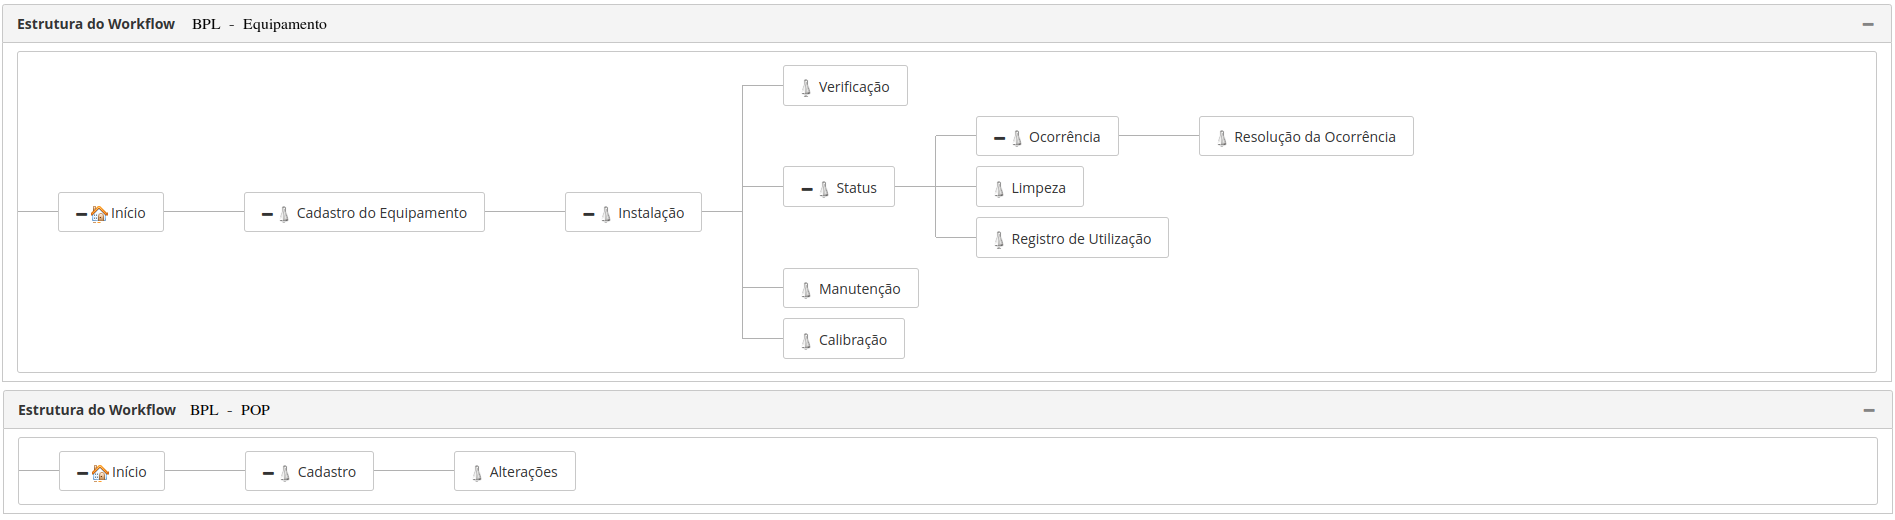
\includegraphics[width=1\textwidth]{imgs/BPL/estrutura.png}
    \caption{Estrutura de dois workflows: BPL - POP e BPL Equipamentos. A atividade inicial destes workflows são as atividades ``Cadastro'' e ``Cadastro do equipamento'', respectivamente.}
    \label{fig:estrutura_workflow}
\end{figure}

\begin{figure}
    \centering
    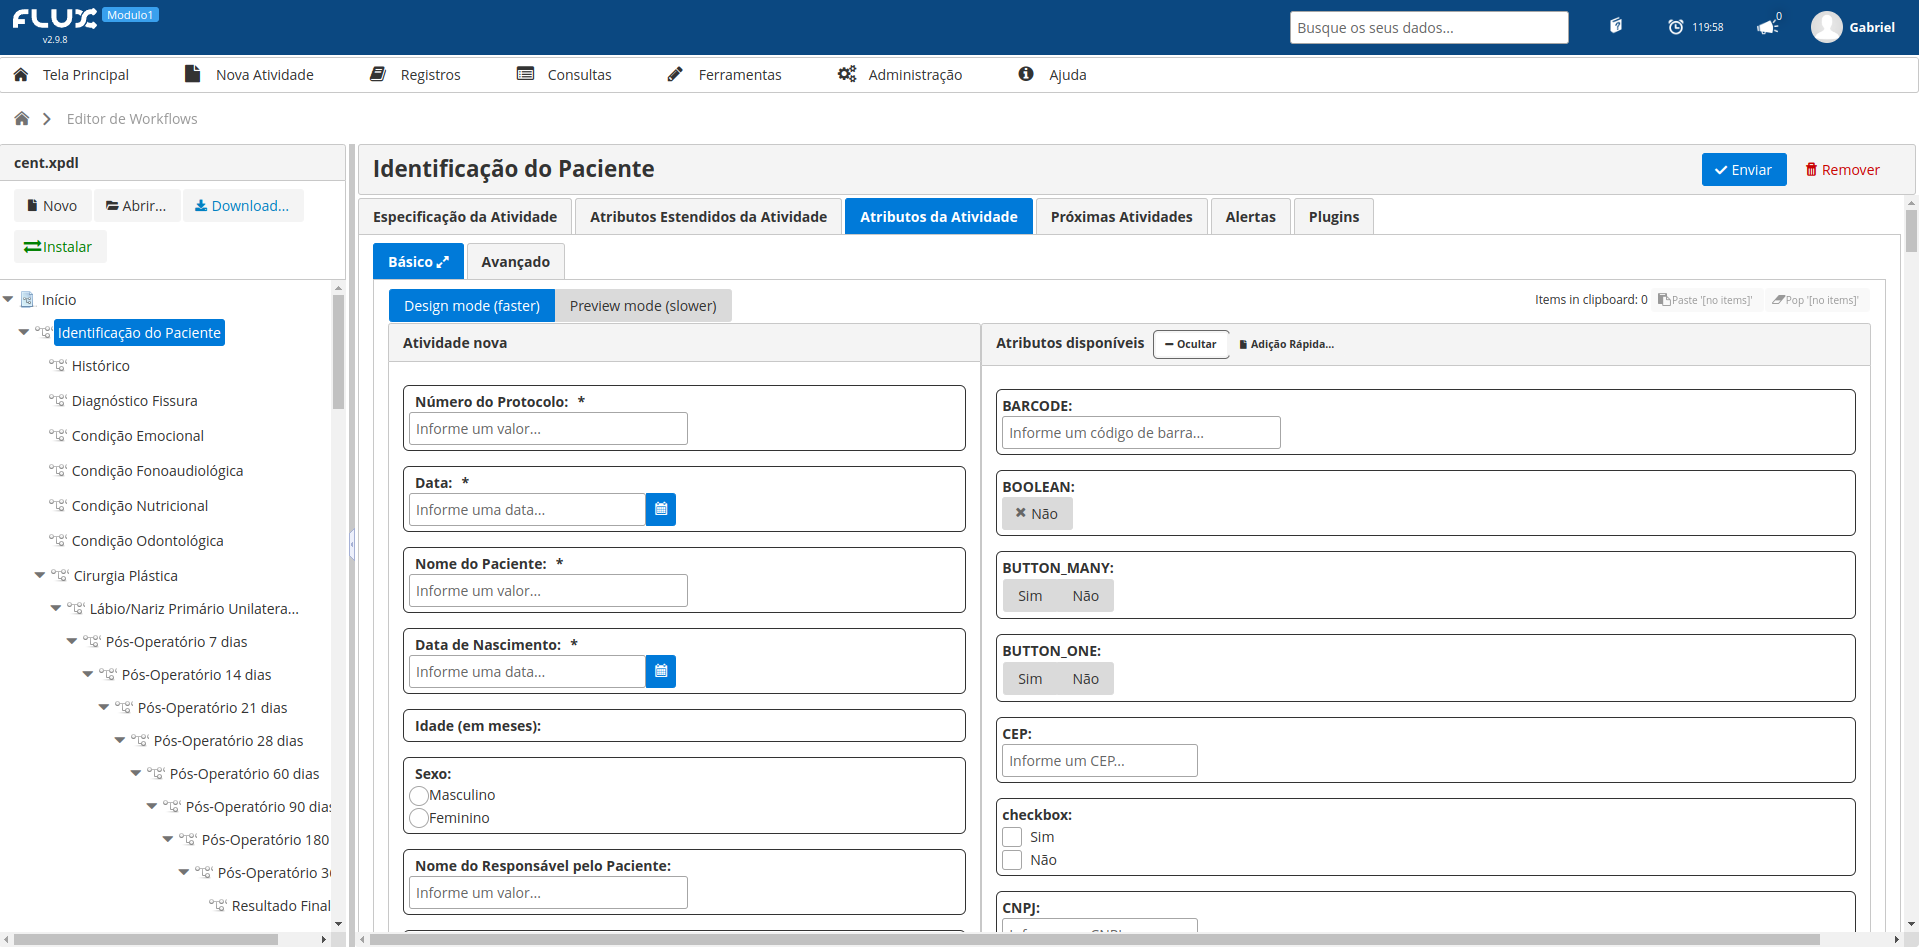
\includegraphics[width=1\textwidth]{imgs/Flux/Workflows/Editor/editor_centrare.png}
    \caption{Visualização da primeira atividade do workflow CENTRARE e seus atributos no editor de workflows do LIMS Flux.}
    \label{fig:editor_centrare}
\end{figure}

\subsubsection{Transições} \label{sec:transitions}

No Flux existe o conceito de transições. Uma transição define uma relação de dependência entre duas atividades. Para que exista uma atividade B filha de A, deve-se existir uma transição entre elas. Cada transição demonstra uma relação de dependência entre as atividades filha e as atividades pai (como visto na figura~\ref{fig:transitions})

Também ocorre a existência de transições entre atividades que não são pais e filhas, que nada mais é a criação de uma transição entre elas. Quando isso ocorre, a transição dita uma correlação de dependência entre duas atividades sem a necessidade delas estarem na mesma subárvore de um workflow.

Uma transição entre duas atividades demonstra uma relação de dependência entre essas atividades, sendo necessário a execução de uma (atividade pai) para que a outra atividade (filha) possa ser executada. Caso existam múltiplas transições de atividades pai para uma filha (por meio deste tipo de transições), a atividade será disponibilizada na execução de qualquer uma das atividades pai da mesma.

\begin{figure}
    \centering

    \begin{subfigure}[b]{0.45\textwidth}
        \centering
        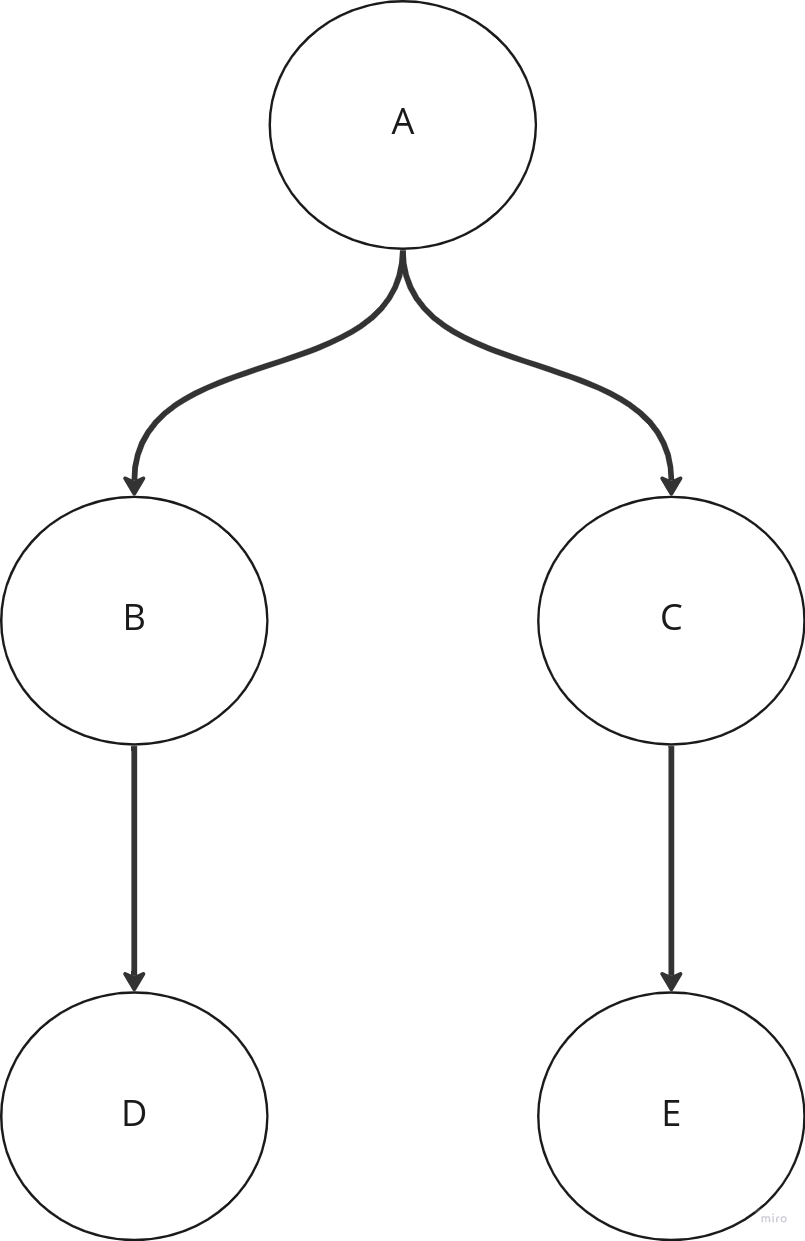
\includegraphics[width=0.6\textwidth]{imgs/Flux/Transicoes/normal.png}
        \caption{Transições entre atividades. Atividade A é a atividade inicial e tem duas atividades filhas: B e C. Delas, temos a atividade D que é filha de B e a atividade E que é filha de C.}
        \label{fig:transition_normal}
    \end{subfigure}
    \hfill
    \begin{subfigure}[b]{0.45\textwidth}
        \centering
        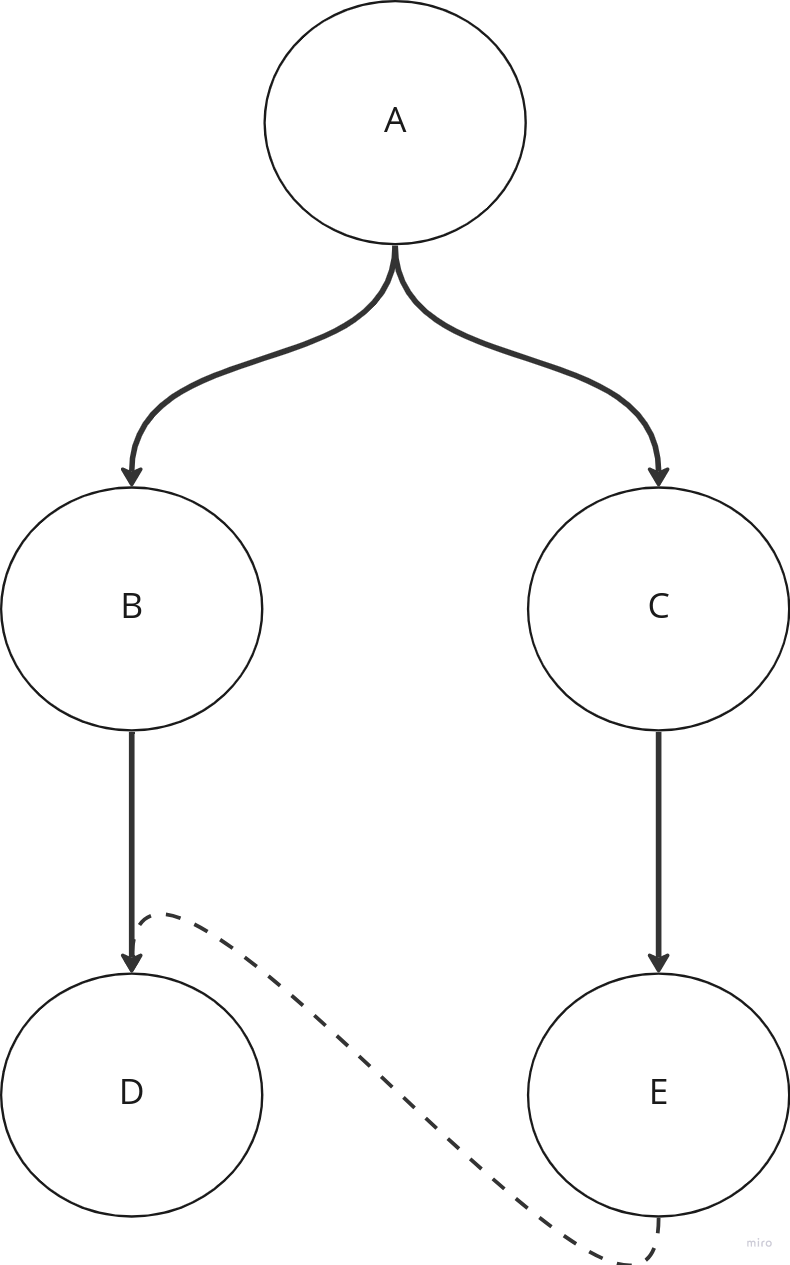
\includegraphics[width=0.6\textwidth]{imgs/Flux/Transicoes/referencia.png}
        \caption{Neste exemplo temos as mesmas transições mostradas em~\ref{fig:transition_normal}, mas com uma transição da atividade E para a atividade D (demonstrada pela seta pontilhada). A atividade D será disponibilizada quando o usuário executar a atividade B OU quando executar a atividade E.}
        \label{fig:transition_ref}
    \end{subfigure}
    \caption{Demonstração de transições entre atividades dentro do Flux. Cada atividade é representada por um circulo e cada seta entre círculos representa uma transição.}
    \label{fig:transitions}
\end{figure}

\subsubsection{Usuários do Flux}

Existem dois tipos de usuários dentro do Flux: Usuários administradores e usuários comuns.

Usuários administradores podem gerenciar todos os quesitos do LIMS para que ele seja moldado para a organização a que pertence. Administradores podem criar workflows dentro do software, configurar permissões de usuários comuns sobre o acesso deles a atividades, instâncias e workflows, além de gerenciar as contas dos próprios usuários comuns.

Os usuários comuns são aqueles que apenas executarão os workflows criados pelos administradores. O usuário comum só poderá visualizar, aprovar, executar, gerar relatórios de atividades que lhe foi dado permissão pelos administradores.

Múltiplos usuários podem executar instâncias diferentes ou até mesmo a mesma instância de um workflow utilizando o Flux. Desta maneira, pode-se integrar múltiplos participantes de um mesmo processo para executarem em paralelo atividades que façam parte do mesmo BPM.

\subsubsection{Grupos de usuários}

O Flux também permite a criação de grupos de usuários. A criação de grupos é feita pelo usuário administrador, que pode gerenciar quais usuários pertencem a que grupos.
Estes grupos criados facilitam a atribuição de permissões em massa para workflows que serão compartilhados com muitos usuários.
Um usuário pode pertencer a um ou mais grupos como demonstrado na figura~\ref{fig:user_edit}.

\begin{figure}
    \centering
    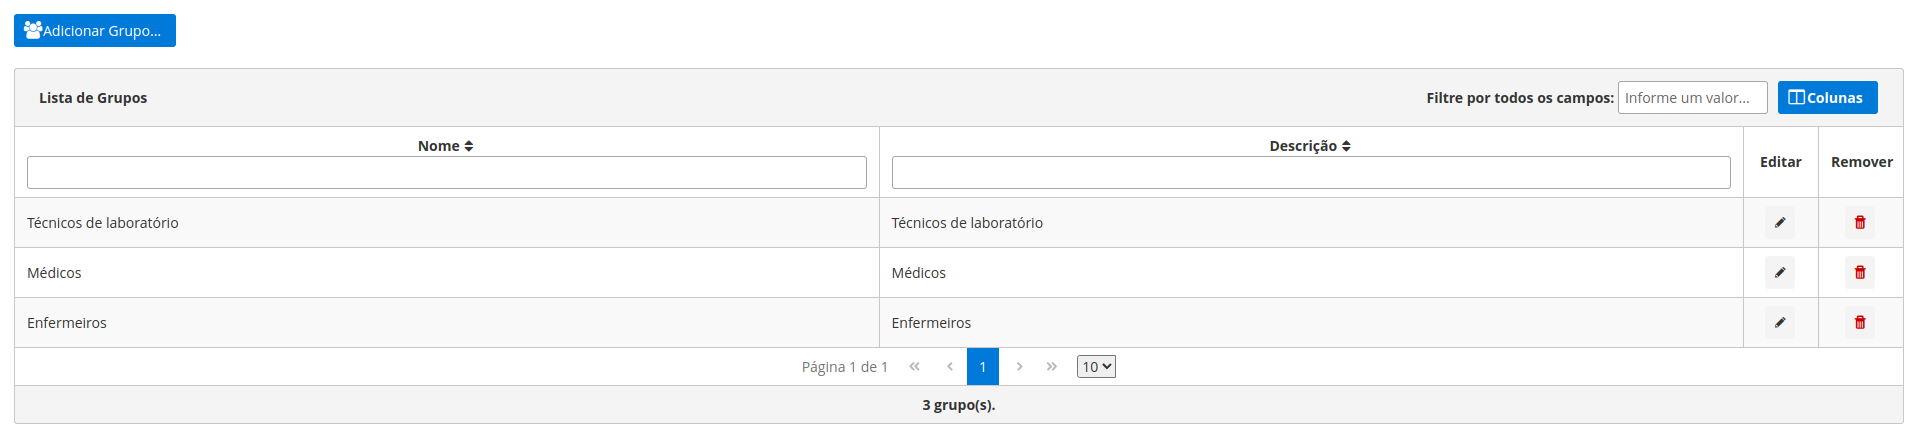
\includegraphics[width=\textwidth]{imgs/Flux/Grupos/listaDeGrupos.png}
    \caption{Lista de grupos criado em um sistema LIMS}
    \label{fig:groups_list}
\end{figure}

\begin{figure}
    \centering
    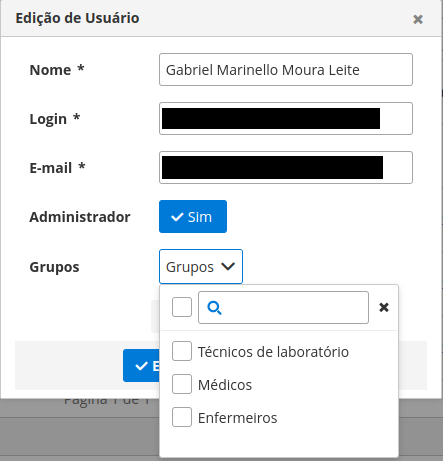
\includegraphics[width=\textwidth, height=7.5cm, keepaspectratio]{imgs/Flux/Usuarios/edicaoUsuario.png}
    \caption{Edição de um usuário. Percebe-se que o usuário pode ser adicionado a um ou mais grupos pela lista de seleção apresentada pela interface no canto inferior da figura.}
    \label{fig:user_edit}
\end{figure}

\subsubsection{Sistema de permissões}

O Flux implementa um sistema de permissões completo, com diferentes níveis de permissão para atividades, instâncias e workflows.
Um usuário administrador do sistema pode gerenciar tais permissões por meio da interface de permissões, que permite a configuração de permissões tanto para usuários individuais quanto para grupos de usuários (demonstrado na figura~\ref{fig:permission_interface}).

Existem 5 níveis de permissão no sistema hoje:

\begin{itemize}
    \item Visualização: Permite ao usuário visualizar a atividade.
    \item Executar: Permite ao usuário inserir dados em uma atividade e executá-la (Gravá-la no banco de dados).
    \item Editar: Permite que o usuário edite dados de uma atividade já executada.
    \item Aprovar: Quando uma atividade for executada, seja pelo usuário com permissão ou por outro usuário, permite que o usuário aprove os dados da atividade. Atividades filhas só ficarão disponíveis com esta aprovação.
    \item Gerar Relatório: Permite que o usuário imprima um relatório da atividade.
\end{itemize}

Cada uma dessas permissões podem ser atribuídas separadamente para cada usuário e/ou grupo de usuários, para cada atividade de um workflow (como demonstrado na figura~\ref{fig:permission_activity_interface}).

Caso um usuário pertença a um grupo de usuários que detêm um conjunto de permissões, este usuário irá receber todas as permissões atribuídas àquele grupo. Com isso, há uma maior facilidade para atribuição de permissões para múltiplos usuários ao mesmo tempo com a criação de grupos diferentes para cada setor da organização, já que pode existir um número grande de atividades no workflow modelado.

\begin{figure}
    \centering
    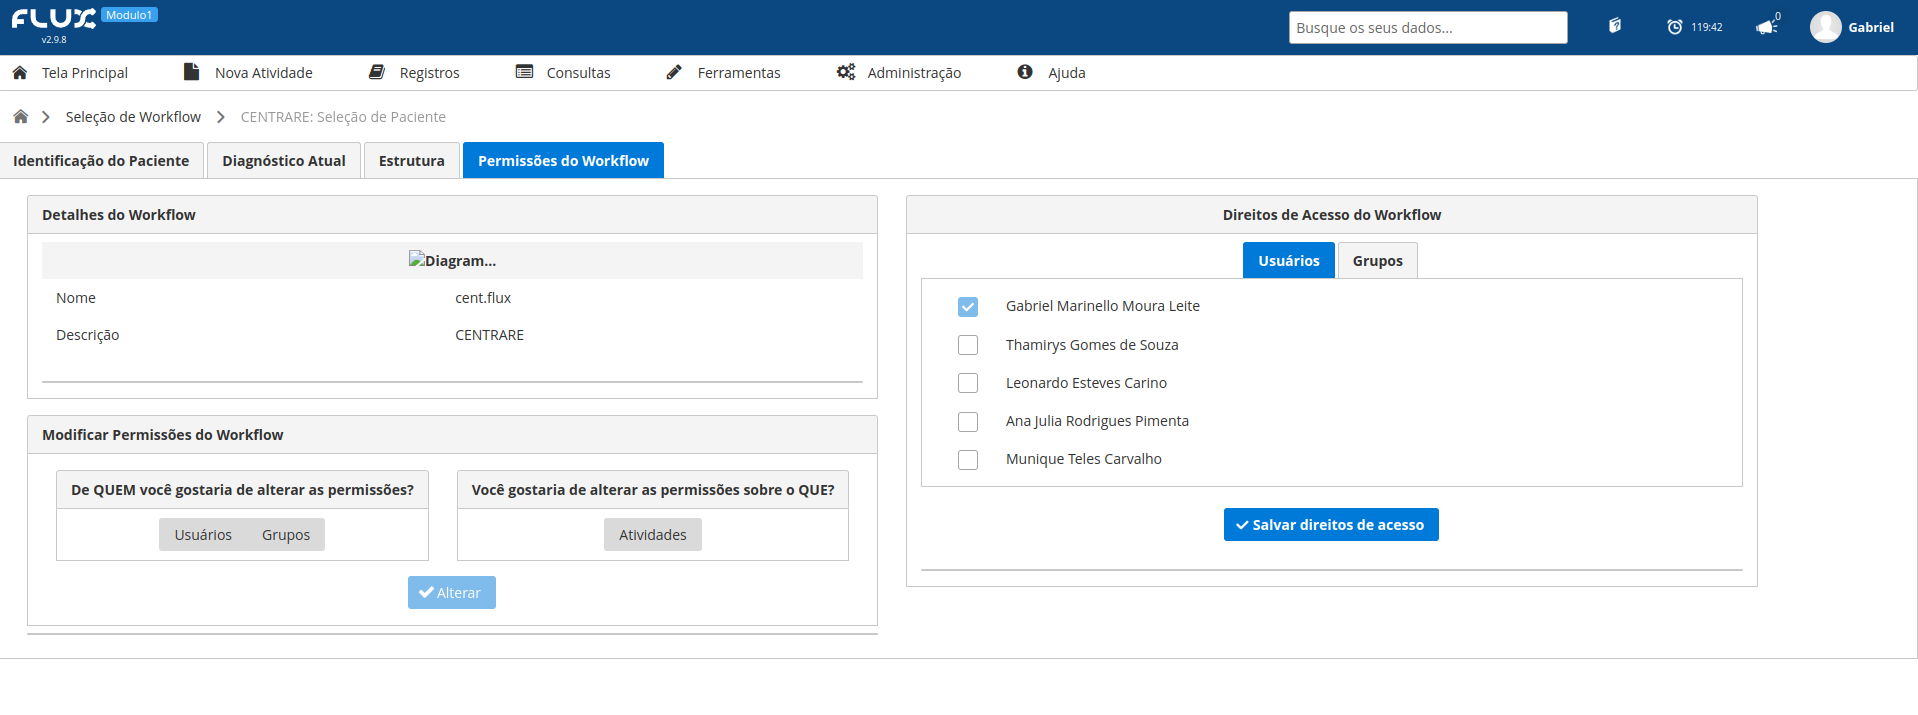
\includegraphics[width=\textwidth]{imgs/Flux/Permissoes/telaPermissoesCENTRARE.png}
    \caption{Interface para alteração de permissões de um workflow (neste caso, do workflow CENTRARE). Caso um usuário não tenha nenhuma permissão em um workflow, o workflow não aparece na interface deste usuário (Usuários desmarcados no canto direto da tela).}
    \label{fig:permission_interface}
\end{figure}

\begin{figure}
    \centering
    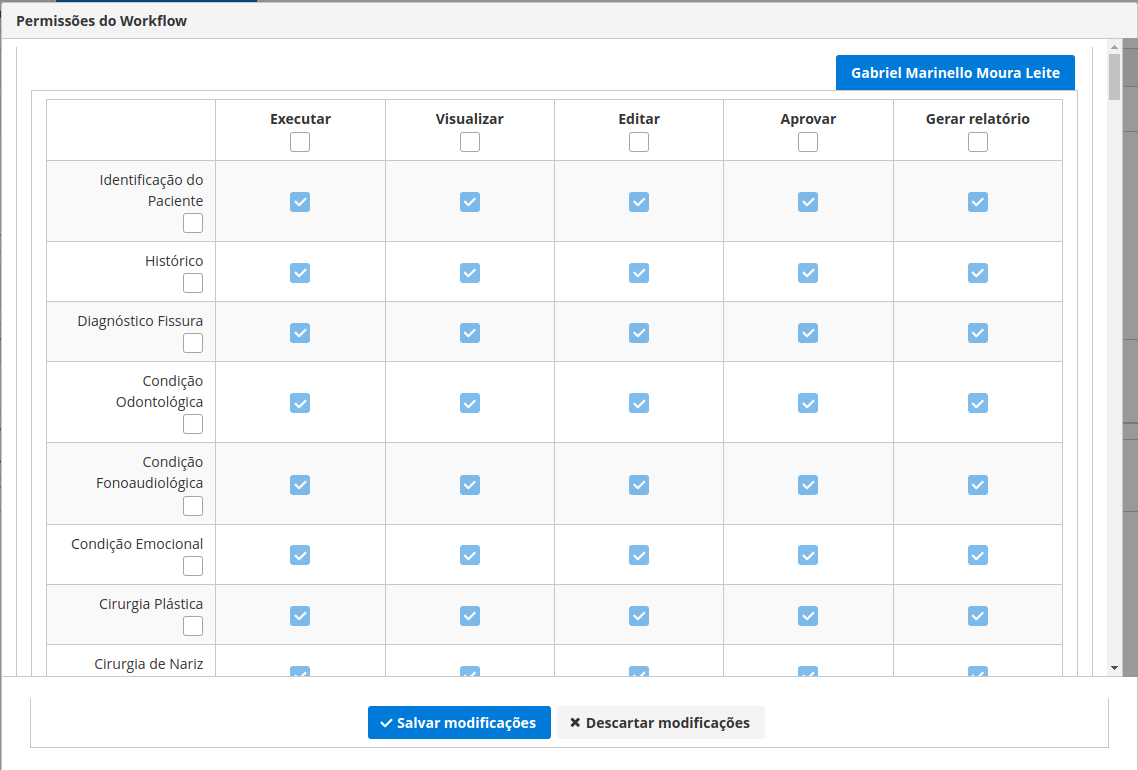
\includegraphics[width=\textwidth]{imgs/Flux/Permissoes/telaPermissoeAstividadesCENTRARE.png}
    \caption{Tela para adição de permissões em atividades do workflow CENTRARE. O usuário administrador pode atribuir permissões diferentes para cada atividade, para cada usuário ou grupo de usuários.}
    \label{fig:permission_activity_interface}
\end{figure}
\section{Workflows Dinâmicos}

\subsection{Proposta}

\subsubsection{Troca de ordem de atividades}

% Troca de ordem de atividades

% O que isso traz para os BPMs

% Isso já é possibilitado pelos BPMs?

Isso já pode ser feito com BPMs na parte de modelagem do mesmo, mas com grandes ressalvas nas partes de segurança, automação e eficiência do mesmo, já que as atividades do BPM podem ter dependências entre si. Isso já é tratado pelo Flux, disponibilizando as informações de maneira a apenas acelerar a visualização das variáveis pelo usuário

% O que isso traz para os usuários

A reordenação do workflow acelera o acesso do usuário a partes que realmente importam para ele no momento, alterando a interface já existente para acatar às necessidades do usuário.

% O que isso traz para os LIMS

Como os LIMS tem o grande problema de ter uma interface complexa, com muitos dados sendo mostrados na tela e uma dificuldade dos usuários a se adaptar e utilizar o LIMS \R, com a alteração da interface para mostrar ao usuário a atividade e os dados requisitados, removemos complexidade na busca de informações dentro do software, aumentando a eficiência na busca de informações.

% Porque isso é necessário?

Isso é necessário pois a premissa de um LIMS que utiliza BPM dentro de uma área laboratorial é a otimização de processos de negócio e aumento de eficiência dos trabalhos. Com a alteração da interface, podemos obter este resultado.

\subsection{Problema}

Embora os sistemas LIMS possam ser uma ferramenta valiosa para gerenciar e rastrear dados em laboratórios, eles podem apresentar alguns desafios, como a complexidade na sua utilização, com necessidade de quantidades significativas de conhecimento e treinamento~\cite{Avery2000ProductGuide.}.

Um dos grandes problemas que ele pode trazer para a área laboratorial ou médica é a falta de personalização: Para atender às necessidades de laboratórios específicos, os LIMS precisam ser altamente personalizáveis.

Os LIMS tem como finalidade serem uma ferramente para facilitar a coleta, armazenamento e análise de dados em laboratórios. Com esta capacidade, o LIMS permite que usuários tenham informações valiosas sobre experimentos, amostras e instrumentos utilizados na área em que está implementado.

O LIMS também pode ajudas a garantir a qualidade dos dados, melhorar a rastreabilidade e a conformidade regulatória e, com a disponibilização das informações em um ambiente centralizado, aumentar a cooperatividade entre equipes e departamentos.

A personalização da interface do sistema LIMS desempenha um papel crucial na facilitação da coleta e análise dos dados disponíveis. Com uma interface personalizada, os usuários podem ajustar o sistema para atender às suas necessidades específicas, melhorando a eficiência e a usabilidade do sistema.

Por exemplo, esta personalização pode disponibilizar informações relevantes naquele momento para o usuário que esteja procurando por dados específicos de um fluxo de trabalho que este gerencia.

Este recurso pode ajudar, também, a simplificar a navegação do sistema, permitindo que os usuários acessem rapidamente as informações que precisam. Isso pode ser particularmente útil para equipes que trabalham em vários projetos ou em diferente áreas de um laboratório, como no caso de um gerente laboratorial.
\subsection{Solução}

Em resposta à necessidade dos LIMS aumentarem a eficiência de obtenção de dados, foi criada uma solução de workflows dinâmicos, que mudam a forma como as informações são apresentadas e disponibilizadas ao usuário.
Com uma interface adaptável e intuitiva, a solução permite ao usuários acessar e interagir com informações essenciais de maneira rápida e eficiente, melhorando a experiência do usuário.

O usuário tem a possibilidade de escolher, dentre todas as atividades disponíveis para sua visualização, a centralização da atividade escolhida para que ela seja o ponto central do fluxo de trabalho. Com isso, o usuário pode facilmente navegar para outras áreas relevantes da interface e personalizar o fluxo de trabalho de acordo com suas necessidades específicas de forma mais rápida do que seguindo o fluxo de trabalho original.

A rápida disponibilização de informações ao usuário resulta em uma série de ganhos, incluindo maior eficiência dos trabalhos feitos dentro do LIMS, já que workflows podem ser feitos com essa funcionalidade em mente, menor gasto com treinamento no uso do LIMS, já que uma interface dinâmica pode deixar a navegação mais intuitiva e aumento da produtividade do usuário com as informações disponibilizadas mais rapidamente.

O usuário deve, no entanto, saber onde as informações estão contidas dentro do fluxo do trabalho existente para selecionar a atividade correta que contém as informações desejadas. Com isso, a interface se altera para que o fluxo de trabalho seja centralizado na atividade que o usuário deseja.

As informações são disponibilizadas como se a atividade centralizada virasse a atividade inicial do workflow, ocorrendo um ``giro" da atividade selecionada, transformando a atividades pais em atividades filhas da mesma, como podemos ver na figura~\ref{fig:primeira_implementacao}.

\begin{figure}
    \centering
    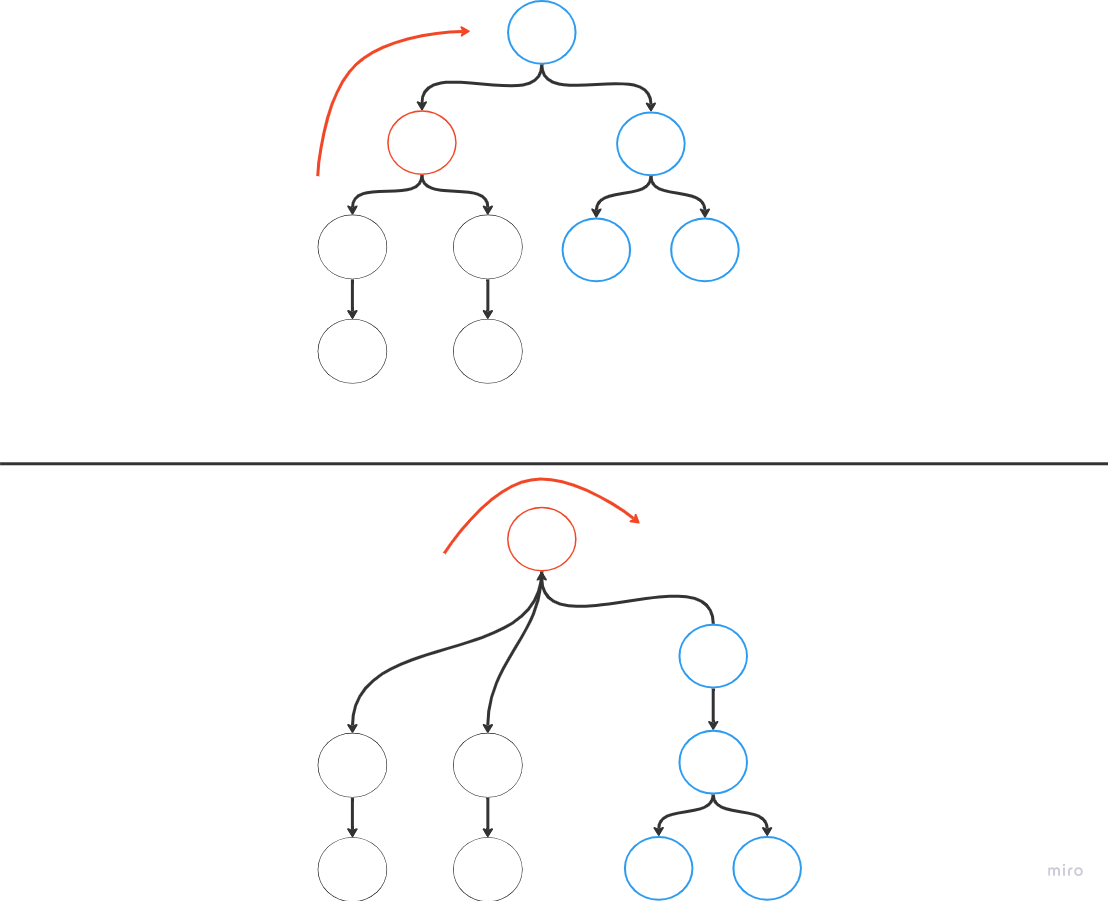
\includegraphics[width=1\textwidth]{imgs/Implementacoes/primeiraImplementacao.png}
    \caption{Representação da implementação de workflows dinâmicas. Na imagem de cima, podemos ver a implementação original de um workflow genérico que está prestes a ser reconstruído. A atividade em vermelho será utilizada como atividade focada apelo usuário. Com isso, a seta em vermelho representa o ``giro" que o workflow faz para que a atividade selecionada vire a primeira atividade do workflow.}
    \label{fig:primeira_implementacao}
\end{figure}
\section{Múltiplos workflows atrelados}

\subsection{Múltiplos pontos de início de um workflow}

% Separação de setores do workflow em categorias de usuários

% O que isso traz para os BPMs?

% Isso já é possibilitado pelos BPMs?

Nos BPMs, não existem múltiplas atividades iniciais, já que um processo consiste de um início, e só a partir dele temos como dar progresso ao modelo de negócios. Com isso, a adição de múltiplas atividades iniciais que podem ser iniciadas por pessoas diferentes adiciona uma ferramenta a modelagem dos workflows.

% O que isso traz para os usuários

A utilização de múltiplos inícios para BPMs facilita o compartilhamento de partes de processos de negócio que podem se repetir entre diferentes BPMs. As atividades repetidas podem ser reutilizadas em cada BPM e compartilhadas caso as informações sejam pertinentes para os BPMs envolvidos.

O compartilhamento de atividades permite que os usuários trabalhem juntos de forma mais colaborativa. Quando um usuário executa uma atividade que é compartilhada com outros BPMs, esta atividade e as informações entradas na execução são disponibilizadas para os usuários que tenham permissão, fornecendo informações sobre o trabalho realizado e permitindo que continuem a trabalhar de forma eficiente.

Após a execução desta atividade compartilhada, outros usuários podem continuar o seu próprio fluxo de trabalho, não necessariamente disponibilizando este fluxo para a pessoa que executou a atividade em si. Isso é possível com a utilização de um sistema de permissões implementado no LIMS. Um exemplo deste tipo de colaboração pode ser visto na figura~\ref{fig:arvore_medico_tecnico}.

\begin{figure}
    \centering

    \begin{subfigure}[b]{0.45\textwidth}
        \centering
        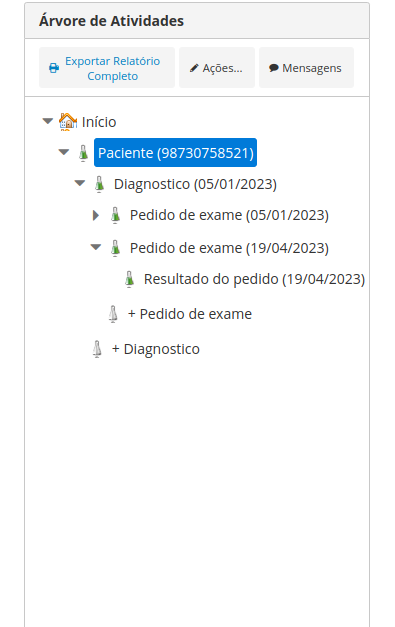
\includegraphics[width=0.8\textwidth]{imgs/Exemplo-Mestrado/arvore_medico.png}
        \caption{Visualização do workflow pela visão do médico, que não tem permissão de visualizar atividades de execução do pedido de exame.}
        \label{fig:arvore_medico}
    \end{subfigure}
    \hfill
    \begin{subfigure}[b]{0.45\textwidth}
        \centering
        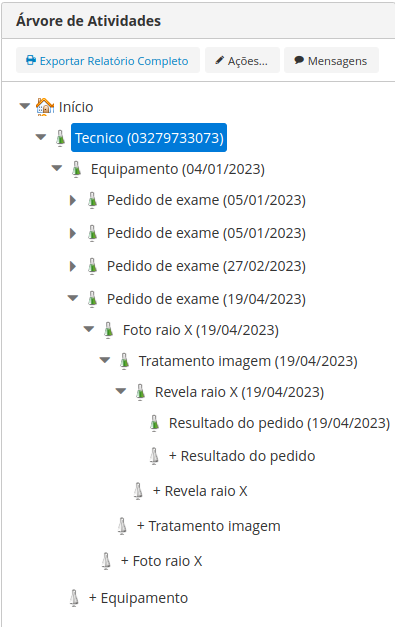
\includegraphics[width=0.75\textwidth]{imgs/Exemplo-Mestrado/arvore_tecnico.png}
        \caption{Visualização do workflow pela visão do técnico de laboratório, que executa as atividades do pedido de exame e executa também o resultado do pedido, disponibilizando para a visualização do médico.}
        \label{fig:arvore_tecnico}
    \end{subfigure}
    \caption{Demonstração de transições entre atividades dentro do Flux. Cada atividade executada é representada uma linha com a imagem de um frasco com líquido verde. Cada mudança de espaçamento entre as atividades mostra que existe transições entre a atividade sem a mudança de espaçamento e as com mudança de espaçamento.}
    \label{fig:arvore_medico_tecnico}

\end{figure}

Um exemplo disso é em um pedido de exame de sangue de um médico para um laboratório, que irá examinar a amostra e fornecer um resultado ao médico. Este médico irá executar uma atividade de pedido de exame que será disponibilizada para o laboratório. Com esta atividade, o laboratório pode executar atividades seguintes de análise do pedido e entregar um resultado ao médico.

% O que isso traz para os LIMS

A integração desta nova ferramenta a um LIMS melhora a eficiência e integração das atividades de um modelo de negócios com o outro, otimizando a troca de informações entre dois fluxos de trabalho. O médico pode receber uma notificação quando o exame ficar pronto, um técnico recebe notificação quando uma amostra chega e pode até ser feita a otimização deste caminho, com a amostra indo direto para uma máquina analisar.

Isso também facilita a utilização do software pelos usuários, já que fica mais intuitivo onde e quando o usuário deve entrar na interface para acessar os dados que são de seu interesse.

% Porque isso é necessário?

\subsection{Usos}

É possível vincular atividades de diferentes BPMs umas as outras por meio do compartilhamento de atividades. Os BPMs que contém atividades compartilhadas devem ser modelados juntos para que toda a execução do fluxo de trabalho possa ser pensado e otimizado visando um processo colaborativo entre os usuários. Os usuários que irão utilizar o workflow poderão receber notificações sobre execuções de atividades compartilhadas por outros usuários. A modelagem também pode ser pensando para envio de notificações para que a execução possa ser feita de maneira mais efetiva. Um exemplo de utilização é a que um cientista pede a análise de uma amostra a um técnico de laboratório, que por sua vez recebe a notificação que o pedido foi feito, deixando disponíveis atividades para execução deste pedido. Quando concluída, o cientista recebe uma notificação de que a análise da amostra foi executada e que ele pode seguir com seu fluxo de trabalho.
\section{Exemplos de Aplicações}

\subsection{Utilização no LIMS Flux}

O LIMS Flux foi utilizado para implementação dos recursos de workflows dinâmicos e da agregação de múltiplos BPMs para troca de informações entre eles. Sua utilização foi feita pela facilidade na criação de workflows dentro do próprio software e a alta personalização disponibilizada.

Como estes recursos alteram como a visualização de um BPM ocorre, foram necessário ajustes para que a implementação de tais recursos fosse feita de maneira correta e consistente, sem que a alteração na visualização deixasse o LIMS com vulnerabilidades de segurança e que as informações estivessem sempre disponíveis quando necessário.

\subsection{Alterações feitas para workflow dinâmicos}

Para que o Flux pudesse focar em uma atividade dentro do workflow, alteramos a definição de instância do programa. Anteriormente, instâncias eram definidas como o inicio do fluxo de trabalho do usuário para execução do BPM.

Com a implementação de workflows dinâmicos, foi necessário a utilização de instâncias como o ponto de partida de execução do usuário naquele momento, e não necessariamente o inicio do fluxo de trabalho. Instancias ainda podem ser utilizadas seguindo a definição anterior caso o usuário não selecione nenhuma atividade para ser focada (Ou selecione a atividade inicial original).

No software, instâncias ainda são criadas apenas para a atividade original, mas de maneira oculta, para disponibilizar as informações para o usuário de maneira conveniente, é criado uma instância temporária onde a atividade inicial é a atividade selecionada pelo usuário, disponibilizando esta atividade centralizada como ponto de partida para sua execução.

É importante que estas instâncias auxiliares não sejam salvas para que não haja duplicação de dados do workflow e para não ocorrer alterações no BPM original. A ordem das atividades sempre deve seguir a estrutura original do BPM para manter o fluxo desejado quando ele foi modelado.

Se a estrutura do BPM mudar de uma maneira a disponibilizar atividades antes de uma dependência, isso pode causar um fluxo de trabalho errôneo que não segue as restrições modeladas quando o workflow foi implementado no sistema, e isso não pode ocorrer para que o BPM ainda esteja em conformidade com as diretrizes do laboratório.

Para selecionar qual atividade inicial será utilizada na visualização atual, foi alterada a interface para adicionar um seletor de atividades, disponibilizando todas as atividades que o usuário tem permissão de acessar em uma lista ordenada pelo nome da mesma. Nele, temos o nome de todas as atividades do workflow selecionado que o usuário tem a permissão de visualizar.

Caso o usuário não selecione nenhuma atividade, a atividade inicial utilizada será a padrão, deixando o workflow na visualização padrão. Exemplos para esta funcionalidade são mostrados na seção~\ref{sec:dinamic_workflows_examples}.

A árvore de atividades também teve de ser alterada, com a criação de novos tipos de atividades: Atividades pai, ou atividades anteriores. Neste tipo de atividade (Identificados pela cor azul na figura~\ref{fig:centrare_tree_normal_altered}), não é possível executar novas atividades, sendo existentes apenas por motivos de disponibilização de informações pertinentes à execução atual.

Foi necessário a criação deste novo tipo de atividade para disponibilizar informações de atividades anteriores para o usuário, já que as informações podem ser pertinentes para o usuário.

Na mesma figura~\ref{fig:centrare_tree_normal_altered} temos as informações do paciente como primeira atividade da visualização original, podendo ser necessária para preenchimento de próximas atividades da atividade selecionada ``Cirurgia de Nariz''.

\begin{figure}
    \centering
    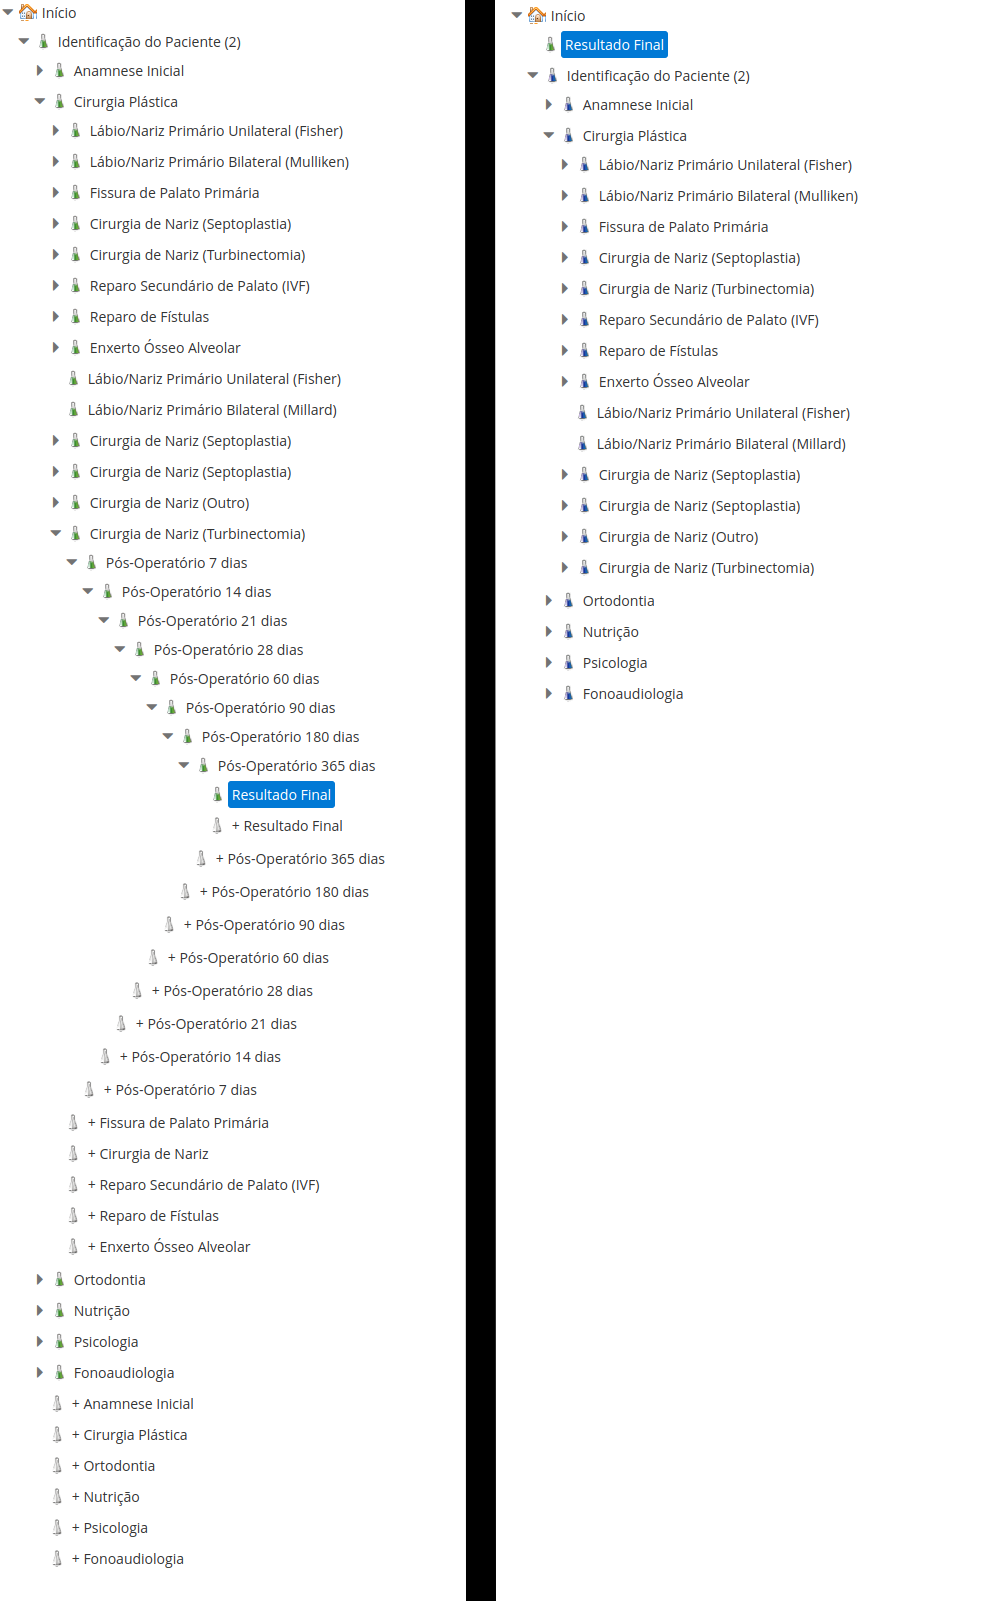
\includegraphics[height=1\textwidth]{imgs/CENTRARE/arvoreNormalEAlterada.png}
    \caption{Imagem demonstrando a árvore de atividades no software original (Esquerda) e a árvore de atividades alterada (Direita). Como podemos ver, a atividade selecionada na esquerda que está no meio do workflow é a mesma atividade selecionada na direita, que agora virou a atividade focada por seleção do usuário. Atividades pai são demonstradas em azul, disponibilizando todas as informações existentes mesmo com a alteração do foco do workflow.}
    \label{fig:centrare_tree_normal_altered}
\end{figure}

\subsubsection{Como funciona}

Quando o usuário seleciona a atividade desejada para ser a atividade inicial, a árvore de atividades é reajustada para que a atividade selecionada seja o foco principal da instância.

Para que isso ocorra, é necessário que a atividade selecionada se torne a atividade inicial, continuando com suas atividades filhas originais mas ganhando uma nova atividade filha: Sua atividade pai. As atividades que eram pais da atividade selecionada se tornam filhas da mesma para que essas informações estejam disponíveis para acesso e para manter a conformidade com a modelagem do BPM já existente.

Para isso, pode-se dizer que ocorre um ``giro'' na árvore de atividades para a direita, tendo todas as atividades anteriores como atividades filhas da selecionada, mantendo a sub árvore de atividades originais intacta. Podemos ver esta característica na figura~\ref{fig:primeira_implementacao}.

No Flux, esta funcionalidade faz com que atividades pai tenham uma cor diferente na interface do usuário (em azul na figura~\ref{fig:centrare_tree_normal_altered}) para que seja claro que as atividades vistas pelo usuário são atividades pai da atividade selecionada. Também é desabilitado a execução de novas atividades a partir das atividades pai.

\subsubsection{Exemplos} \label{sec:dinamic_workflows_examples}

Como exemplo, utilizaremos o workflow modelado para o CENTRARE, que é um fluxo de trabalho para o Centro de Tratamento e Reabilitação de Fissura Labiopalatal e Deformidade Craniofacial do hospital da baleia, em belo horizonte.

Nele, é feito o acompanhamento de pacientes desde o nascimento até a adolescência por múltiplos médicos de diferentes áreas da saúde como odontologia, cirurgia plástica e psicologia. Este fluxo de trabalho é utilizado para o tratamento de lábios leporinos em crianças recém nascidas, com acompanhamento completo pós cirúrgico, familiar e nutricional.

Como este workflow é muito profundo e tem informações de anos acumuladas em um mesmo sistema, ele foi selecionado para a aplicação desta implementação para verificar que as informações ficam mais facilmente disponíveis para os usuários que o utilizam.

Podemos ver a diferença da figura de visualização padrão do fluxo de trabalho (\ref{fig:normalInstance}) e visualização alterada (\ref{fig:changedInstance}). Na primeira imagem, temos uma tabela para seleção de instâncias sem alteração da visualização do workflow. Nela, cada linha na tabela disponibiliza um paciente diferente para seleção.

Na segunda imagem, foi selecionado a atividade ``Cirurgia de Nariz'', disponibilizando todas as cirurgias de Nariz realizadas em todos os pacientes. Em cada linha é disponibilizado certos atributos para visualização para identificar a atividade desejada para obtenção de informações (como visto na figura~\ref{fig:cttx_eqp_calibracao_focada}, cada linha disponibilizando a data de execução da atividade, data de calibração, nome do equipamento e POP).

\begin{figure}
    \centering
    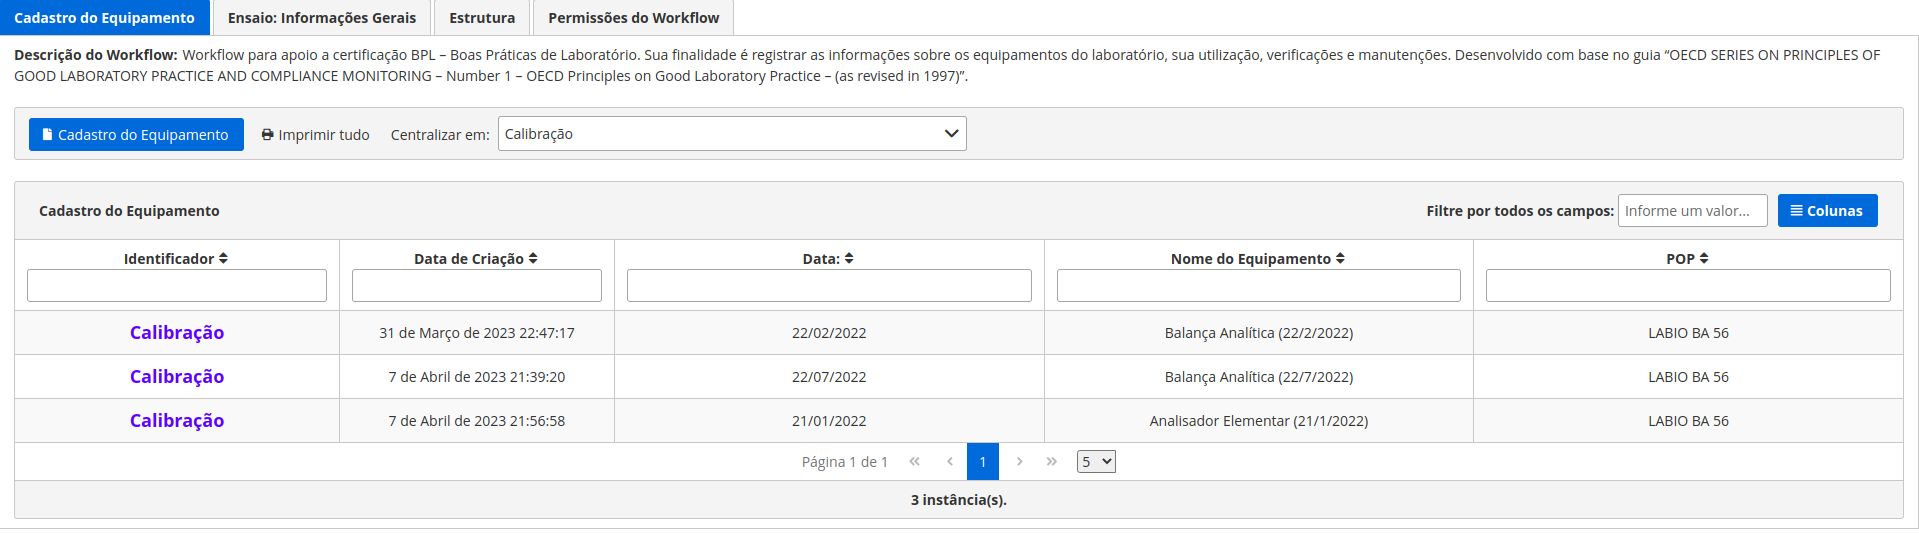
\includegraphics[width=1\textwidth]{imgs/CTTX-EQP/cttx_eqp_calibracao_focada.png}
    \caption{O workflow CTTX-EQP com a atividade compartilhada ``Calibração'' focada.}
    \label{fig:cttx_eqp_calibracao_focada}
\end{figure}

Existem mais atividades do tipo ``Cirurgia de Nariz'' porque, seguindo a modelagem do workflow CENTRARE, existe o cadastro de um paciente que, por sua vez, pode ter feito uma ou mais cirurgias de nariz. Para identificar qual atividade pertence a qual paciente, pode ser adicionado um atributo na atividade que recebe como valor o nome do paciente (ou um identificador único), deixando mais rápido para o usuário identificar a qual instância do workflow original aquela atividade pertence. Esse tipo de identificação foi utilizado no workflow CTTX - EQP que será explicado nas próximas seções.

\begin{figure}
    \centering
    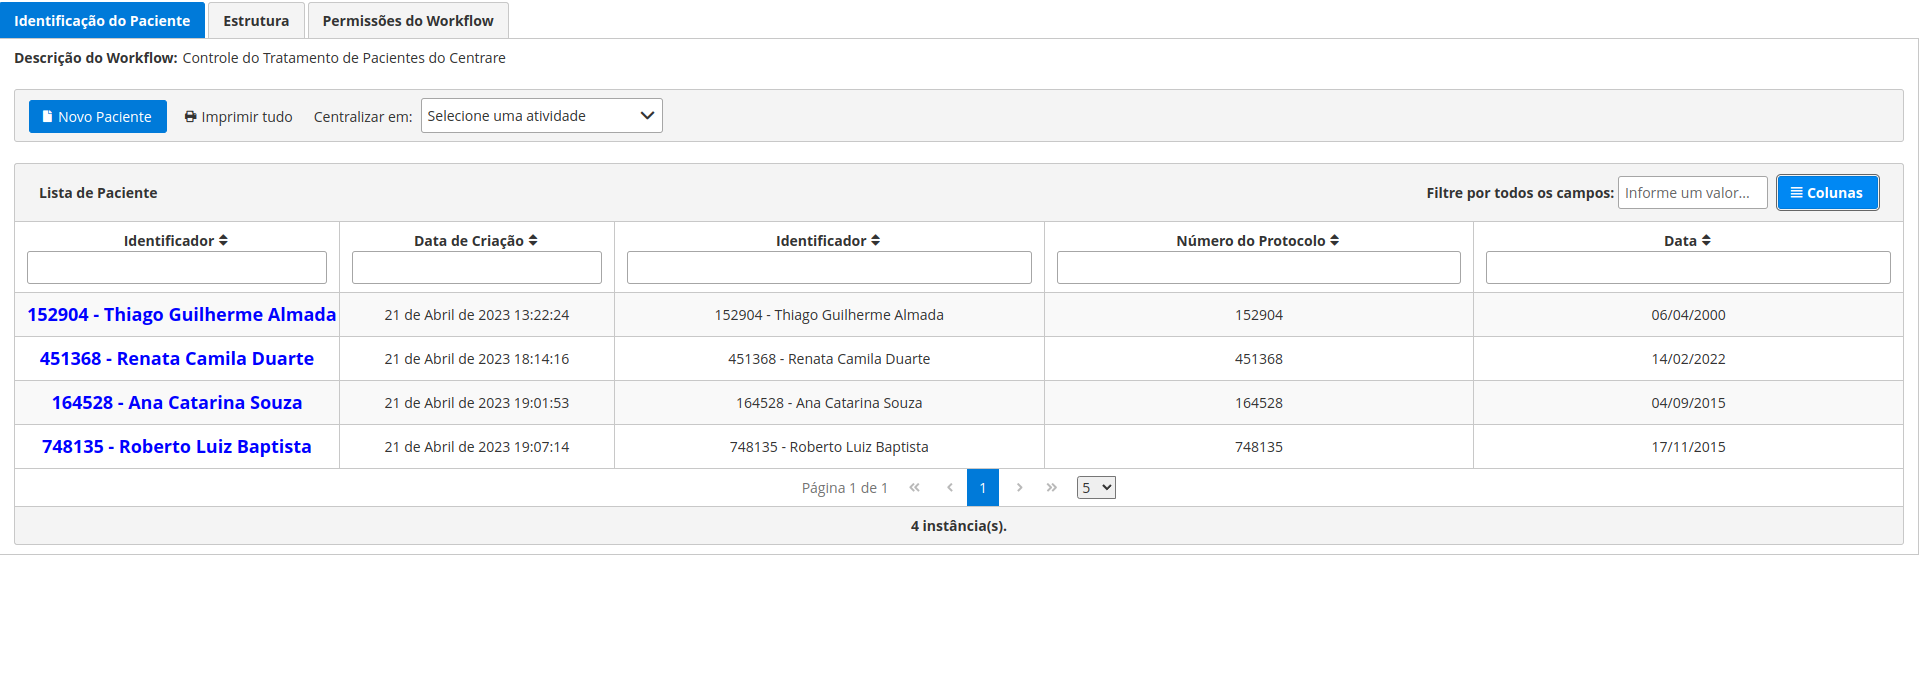
\includegraphics[width=1\textwidth]{imgs/CENTRARE/instanciaNormal.png}
    \caption{Workflow padrão do CENTRARE, sendo sua centralização feita na atividade inicial de ``Identificação do Paciente''}
    \label{fig:normalInstance}
\end{figure}

\begin{figure}
    \centering
    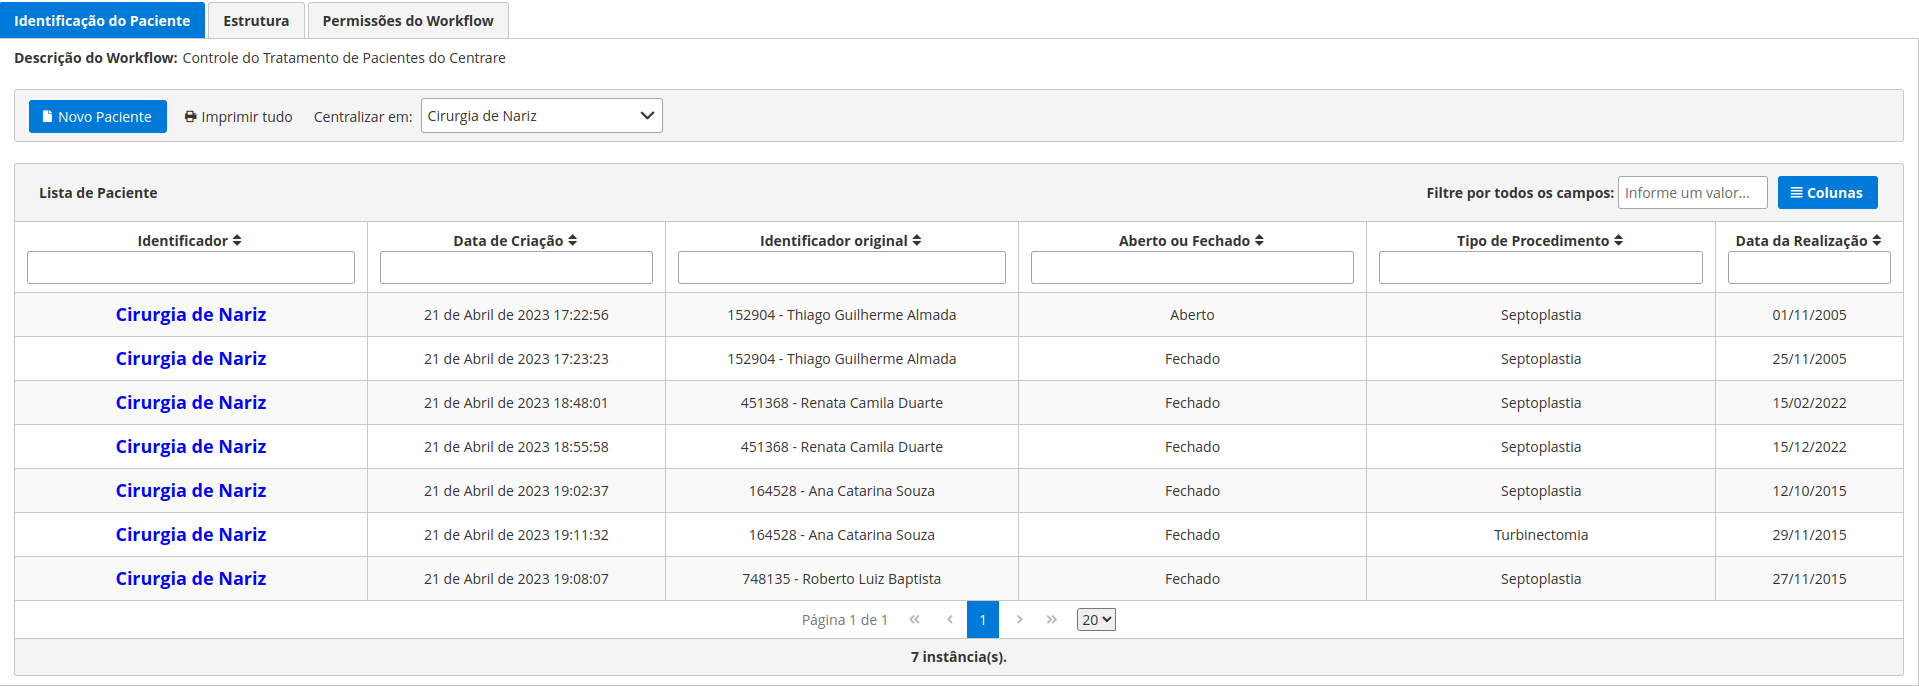
\includegraphics[width=1\textwidth]{imgs/CENTRARE/instanciaAlterada.png}
    \caption{Workflow com visualização centralizada na atividade ``Cirurgia de Nariz, disponibilizando informações da atividade como ``Cirurgião'', ``Aberto ou Fechado'' e ``Topo de Procedimento''}
    \label{fig:changedInstance}
\end{figure}

Ao acessar o workflow, podemos ver pela figura~\ref{fig:centrare_tree_normal_altered} a alteração da árvore do workflow, disponibilizando as atividades anteriores (em azul) para acesso do usuário, disponibilizando informações de outras atividades caso necessário (como a identificação do paciente) e disponibilizando o acesso mais efetivo de atividades filhas dessa atividade.

\subsection{Alterações feitas para múltiplas atividades iniciais}

Enquanto a BPMN permite múltiplas maneiras de iniciar um processo, ela permite apenas uma atividade inicial em um diagrama de processo, representado por um único evento de início.

Como uma organização pode ter múltiplas equipes trabalhando em focos diferentes, é necessário a divisão em diversos workflows para que todos os processos estejam modelados para que fluxos de trabalho possam ser diagramados e executados.

Como um mesmo workflow pode ter troca de informações com alguma parte de outros workflows, foi idealizado uma nova funcionalidade para um workflow no Flux: Múltiplas atividades iniciais que compartilham atividades entre instâncias no meio de sua execução.

Cada possível atividade inicial do workflow pode ser utilizada para criar uma instância diferente do workflow, já que cada uma dessas atividades representa um tipo de execução diferente do workflow (na figura~\ref{fig:segunda_implementacao}, uma atividade inicial é para cadastro de pacientes e a outra para cadastro de técnicos de laboratório).

Com um workflow com múltiplas atividades iniciais, é possível ter atividades que, ao serem executadas, serão disponibilizadas para outros usuários que utilizam este workflow, independente da instância que estiverem executando. Assim, usuários que estão executando atividades em uma parte do workflow (partindo de uma atividade inicial) compartilham informações com outros usuários (partindo de outra atividade inicial).

Com a execução de dois workflows agregados, cada execução iniciando de uma atividade inicial diferente, é possível o compartilhamento das atividades que contém um processo idêntico entre os dois workflows agregados, disponibilizando as informações para as instâncias selecionadas.

Desta forma, aumenta-se a integração do sistema por haver a troca de informações entre processos de trabalho diferentes dentro de uma mesma organização, disponibilizando a cooperação entre usuários do mesmo sistema.

\subsubsection{Como funciona}

Para compartilhar atividades entre múltiplos workflows, é necessário que estes workflows estejam juntos em uma mesma modelagem com múltiplas atividades iniciais.

Para isso, foi alterado o editor de workflows já existente no Flux para que fosse possível criar múltiplas atividades iniciais, uma atividade inicial para cada workflow agregado.
Os workflows não precisam ter atividades compartilhadas para estarem juntos, eles funcionarão como workflows normais, com criação de instâncias e atividades da mesma maneira, apenas estando sob o mesmo nome de workflow e dentro da mesma interface que disponibiliza as informações de um workflow, disponibilizando recursos como busca de informações e geração de relatório dentro do mesmo workflow.

Quando uma atividade deve ser compartilhada entre workflows, é necessário cria-la como filha de uma das atividades que a utilizarão. Logo após a criação da atividade, é necessário criar transições entre todas as atividades pai para que tenham a atividade compartilhada disponível para execução (figura~\ref{fig:transition_ref}).

Existem dois tipos de compartilhamento: Um compartilhamento geral, onde a atividade será compartilhada entre todas as instâncias existentes assim que ela for criada e um compartilhamento seletivo, onde o usuário escolhe qual instância receberá as informações da atividade executada.

No caso do compartilhamento geral, ele é necessário pois atividades podem ser executadas antes de uma instância existir, como por exemplo no workflow de Citotoxicidade (CTTX): Um equipamento pode existir antes de um ensaio de citotoxicidade ser executado.

Para o compartilhamento seletivo, ele é necessário pois em um pedido de exame, o envio do exame deve ser feito para um laboratório específico e não pode aparecer para outros laboratórios, sendo necessário a seleção de qual laboratório receberá o compartilhamento da atividade.

Nos dois casos, a disponibilização de atividades filhas da atividade compartilhada apenas não ocorre quando existir regras de permissões que não deixem certos usuários (ou grupos de usuários) acessar determinada atividade, caso contrário, todas as atividades e as informações contidas nelas serão compartilhadas.
Isso da uma ferramenta poderosa pela combinação do sistema de permissões e compartilhamento de atividades: A requisição de informações e a entrega das mesmas por dois setores diferentes de uma organização.

\subsubsection{Exemplo de pedido de exame}

Vamos utilizar o exemplo de um pedido de exame em um workflow médico e o recebimento deste pedido de exame e execução do mesmo.
Um médico cria uma instância de paciente, cadastrando-o e seguindo o fluxo de trabalho comum de atendimento.
O laboratórios do hospital também tem seu próprio workflow, onde são cadastrados equipamentos para análise de amostras.
Antes, os workflows ficariam separados, sem comunicação entre eles.

Com o novo recurso implementado, os workflows podem compartilhar atividades como o pedido de exame: O médico tem a permissão de executar o pedido de exame, mas ele não aprova a atividade. Quem irá aprovar a atividade é o técnico de laboratório.

O técnico de laboratório recebe uma notificação que a atividade foi executada e pode aprovar ou reprovar a atividade.
Aprovando a atividade, o técnico continua com seu workflow normalmente até o resultado.
Caso o médico tenha permissão de visualizar as atividades entre o pedido de exame e resultado do exame, o médico poderá ver todo o processo de análise.
Caso contrário, o sistema de permissões controla o que o médico poderá ver, que será o pedido de exame e o resultado do exame.

Assim, a árvore de atividades, caso o médico tenha permissão de visualizar apenas o pedido de exame e a execução, fica da maneira representada na figura~\ref{fig:segunda_implementacao}. Um exemplo real será demonstrado na seção~\ref{sec:cttx_bpl}

\begin{figure}
    \centering
    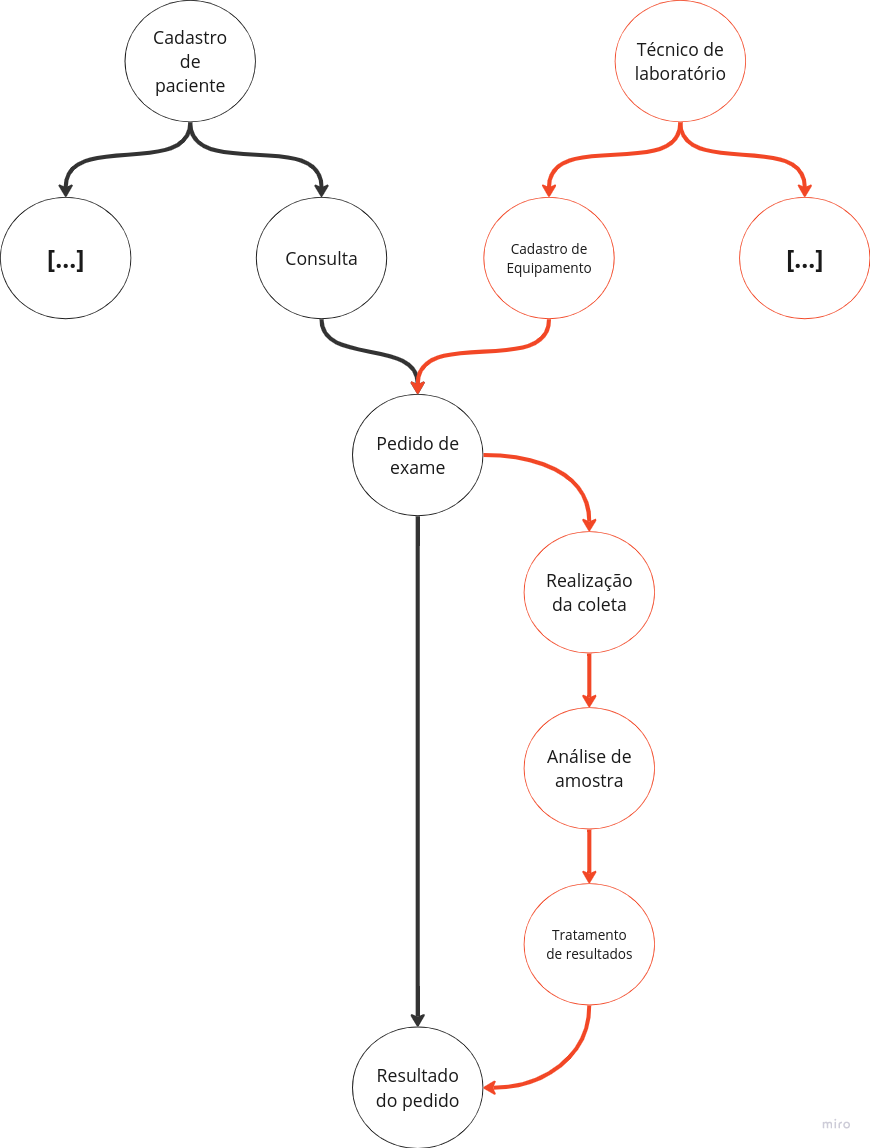
\includegraphics[width=0.65\textwidth]{imgs/Exemplo/exemplo_pedido_exame.png}
    \caption{Representação da implementação de múltiplas atividades iniciais. Neste exemplo, temos a instância de pacientes em preto e em vermelho temos o workflow do técnico de laboratório. Podemos ver que as atividades em preto e vermelho são compartilhadas, e apenas o técnico tem permissão de visualização das atividades entre o pedido de exame e o resultado do pedido.}
    \label{fig:segunda_implementacao}
\end{figure}

% Workflow grande feito no Flux

\subsection{CTTX e BPL Equipamentos} \label{sec:cttx_bpl}

Um outro exemplo utiliza os workflows CTTX (Citotoxicidade) e BPL (Boas Práticas de Laboratório) - Equipamentos. Estes dois workflows necessitam de troca de informações entre eles: BPL - Equipamentos precisa informar sobre a calibração de equipamentos para utilização no workflow CTTX.

Para isso, foi aplicado a implementação de compartilhamento de atividades entre a atividade de calibração do equipamento, disponibilizando a atividade ``Leitura de Absorbância: Perfil Inicial de Citotoxicidade (Range Finder)'' somente após uma atividade calibração do equipamento (Como podemos ver na figura~\ref{fig:cttx_eqp_structure}).

Utilizando o sistema de permissões do Flux, é possível limitar o acesso de cada tipo de usuário (cientista, técnico de laboratório, gerente de laboratório) para que o usuário tenha acesso apenas a informações relevantes ao seu trabalho. Um usuário responsável pela leitura de absorbância terá permissão para visualizar a calibração dos equipamentos utilizados, mas ele não pode realizar nenhuma calibração.

O técnico de laboratório não poderá executar nenhuma leitura de absorbância, e também não terá permissão para visualizar as atividades, enquanto que um gerente de laboratório pode visualizar todas as informações colocadas nos workflows, podendo alterar o tipo de visualização usando a implementação de workflows dinâmicos para obter informações mais rapidamente.

\begin{figure}
    \centering
    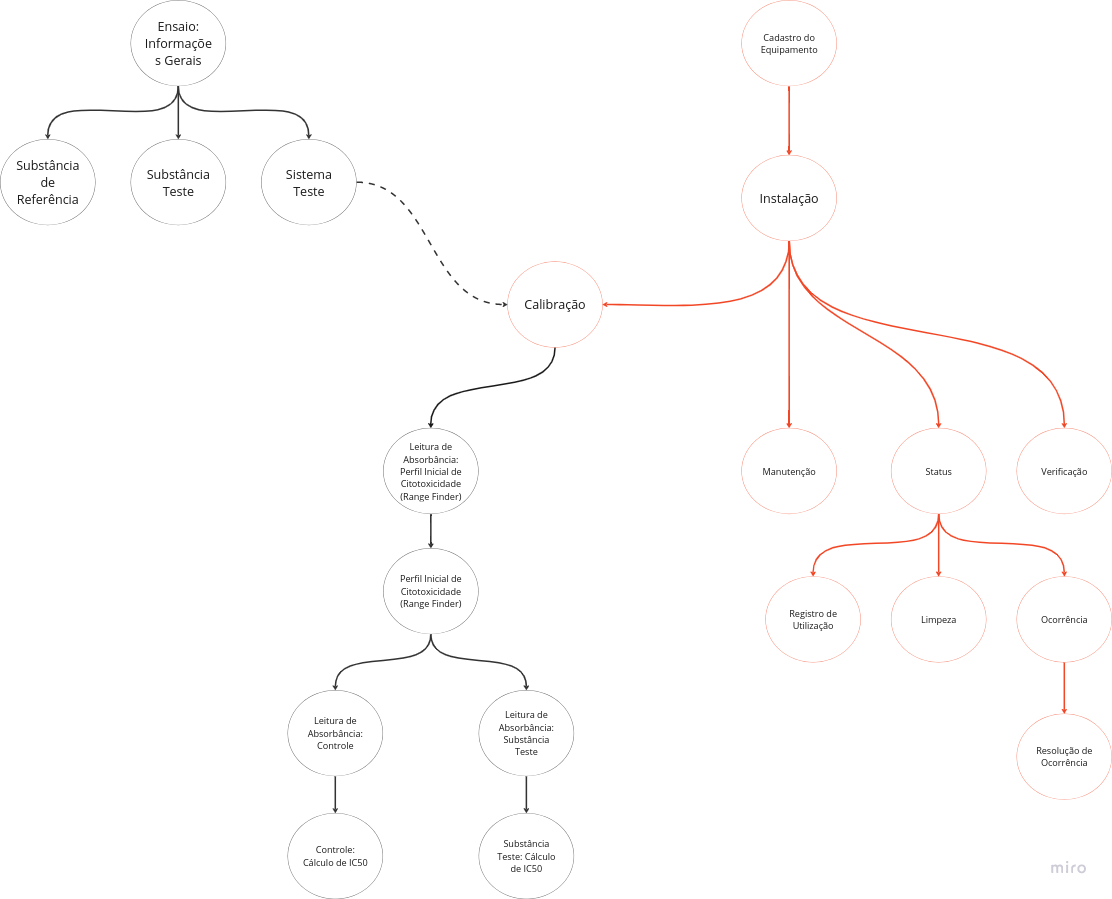
\includegraphics[width=1\textwidth]{imgs/CTTX-EQP/estrutura_cttx_eqp.png}
    \caption{Estrutura dos workflows CTTX e BPL-EQP. O workflow original do CTTX pode ser visto com as setas e círculos de cor preta. A seta pontilhada indica a transição antiga do workflow CTTX, sendo as novas transições entre ``Sistema Teste'' e ``Calibração'', e ``Calibração'' e ``Leitura de Absorbância: Perfil Inicial de Citotoxicidade (Range Finder)'' indicam as novas transições feitas para a comunicação da atividade ``Calibração'' do workflow BPL com o workflow CTTX. A atividade de Leitura de Absorbância só poderá ser realizada quando um equipamento for calibrado.}
    \label{fig:cttx_eqp_structure}
\end{figure}

O equipamento calibrado está identificado por um atributo dentro da atividade de calibração. Este atributo tem uma propriedade que faz o valor ser utilizado no nome da atividade. Caso o equipamento cadastrado tenha o nome de ``Balança Analítica'', a atividade de calibração terá o nome ``Calibração (Balança Analítica)'', com a data da calibração logo ao lado para maior facilidade de busca dos dados (como visto na imagem~\ref{fig:cttx_eqp_calibration}).

\begin{figure}
    \centering
    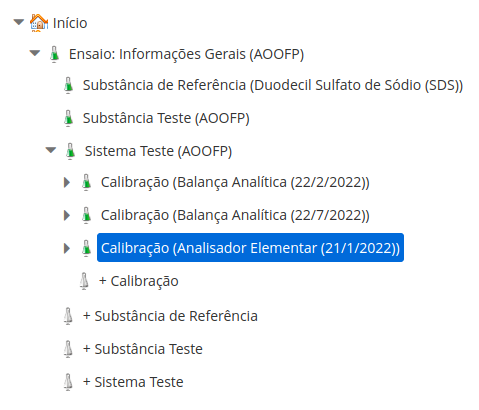
\includegraphics[width=.5\textwidth]{imgs/CTTX-EQP/calibration_tree.png}
    \caption{CTTX com as atividades de calibração de equipamento, identificadas pelo nome do equipamento e data de calibração.}
    \label{fig:cttx_eqp_calibration}
\end{figure}
\subsection{Workflow dentro do Flux que utiliza das funções}

\subsubsection{Workflows BPL}

Os workflows laboratoriais de nome BPL (Boas Práticas de Laboratório) estavam separados em 5 workflows diferentes, já que existiam BPMs diferentes para cada tipo de usuário.
O problema com o BPL é que existem workflows pequenos (pouco profundos, com poucas atividades) e também existem workflows grandes (Com muitas atividades, profundos) e, com isso, surge a dificuldade de disponibilização de dados para diferentes tipos de usuários como a utilização do workflow por gerentes e técnicos de laboratório.

Essa dificuldade existe porque, para cada workflow, deve ser acessado uma página diferentes do LIMS, já que cada um desses workflows representa um sistema diferente para cada usuário.

Com a implementação de compartilhamento de informações entre workflows, conseguimos utilizar estes workflows junto a workflows diferentes para unirmos as boas práticas de laboratório aos workflows que a utilizam, tendo um maior controle de execução de cada um destes fluxos de trabalho, garantindo que todos estão seguindo as normas de BPL, como é o caso do CTTX.

% Para que esta ferramenta fosse mais poderosa, também foi implementado a funcionalidade de múltiplas atividades iniciais no workflow do BPL, fazendo com que workflows dinâmicos pudessem ser centralizados em qualquer atividade que estivesse compartilhada entre instâncias, agregando informações necessárias para execução de um BPM, como calibração de um equipamento de análise de substâncias.

\subsubsection{CTTX e BPL - Equipamentos}

O workflow de Citotoxicidade (CTTX) utiliza o workflow \textit{BPL - Equipamentos} para garantir que equipamentos estejam calibrados e funcionais. Uma atividade deste workflow só deve ser executada quando as calibrações dos equipamentos utilizados estiverem em dia.

Para isso, foi compartilhada a atividade de calibração do workflow \textit{BPL - Equipamentos} com o workflow \textit{CTTX}, implementando este fluxo de trabalho no Flux, adaptando o workflow para que atividades do workflow CTTX apenas estivessem disponíveis para execução após uma calibração.

A estrutura dentro do Flux (Figura~\ref{fig:cttx_bpl_flux}) pode ser acessada dentro do próprio software. Na figura, podemos ver referência à atividade ``Calibração'' nos dois fluxos de trabalho. Para separar quais atividades ficam disponíveis para cada usuário do sistema, é necessário utilizar o sistema de permissões já implementado no Flux para especificar permissões de visualização, execução e aprovação da atividade.

\begin{figure}
    \centering
    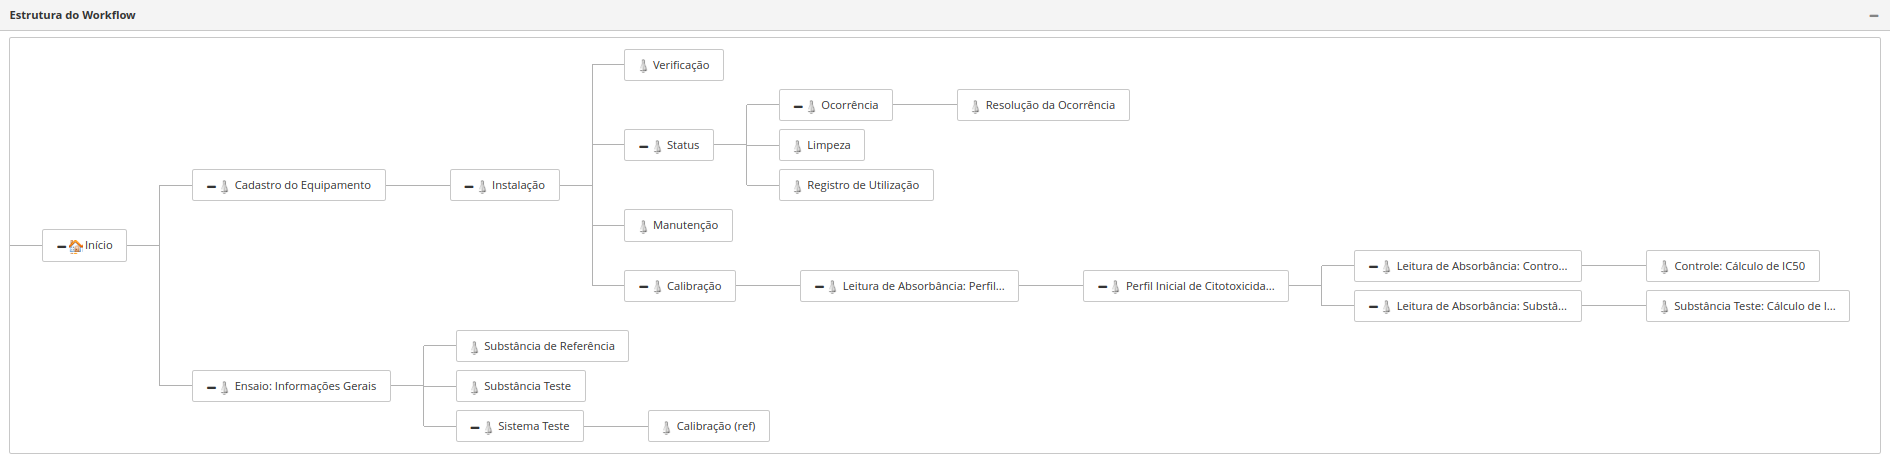
\includegraphics[width=1\textwidth]{imgs/CTTX-EQP/estrutura_cttx_eqp_flux.png}
    \caption{Estrutura do workflow conjunto CTTX com BPL - Equipamentos demonstrada pela interface do Flux. Como podemos ver pela imagem, após a atividade ``Sistema teste'' (canto inferior da imagem), temos a atividade ``Calibração (ref)'', que refere-se a atividade calibração no fluxo de trabalho demonstrado logo acima.}
    \label{fig:cttx_bpl_flux}
\end{figure}

Assim, podem ser separados usuários que irão executar a atividade de calibração do equipamento de usuários que irão realizar os experimentos a partir daquela calibração, diminuindo os erros que podem ocorrer caso as atividades sejam disponibilizadas sem que um equipamento tenha sido calibrado corretamente.

Na visão de um administrador, a mesma atividade selecionada de calibração foi realizada, e as mesmas atividades são disponibilizadas para o usuário (Por ele ter permissão de ver todas as atividades) de maneira automática com o compartilhamento de atividades apresentadas nas figuras~\ref{fig:cttx_executado_calibracao_equipamento} e~\ref{fig:cttx_executado_calibracao_leitura_absorbancia}.

\begin{figure}
    \centering
    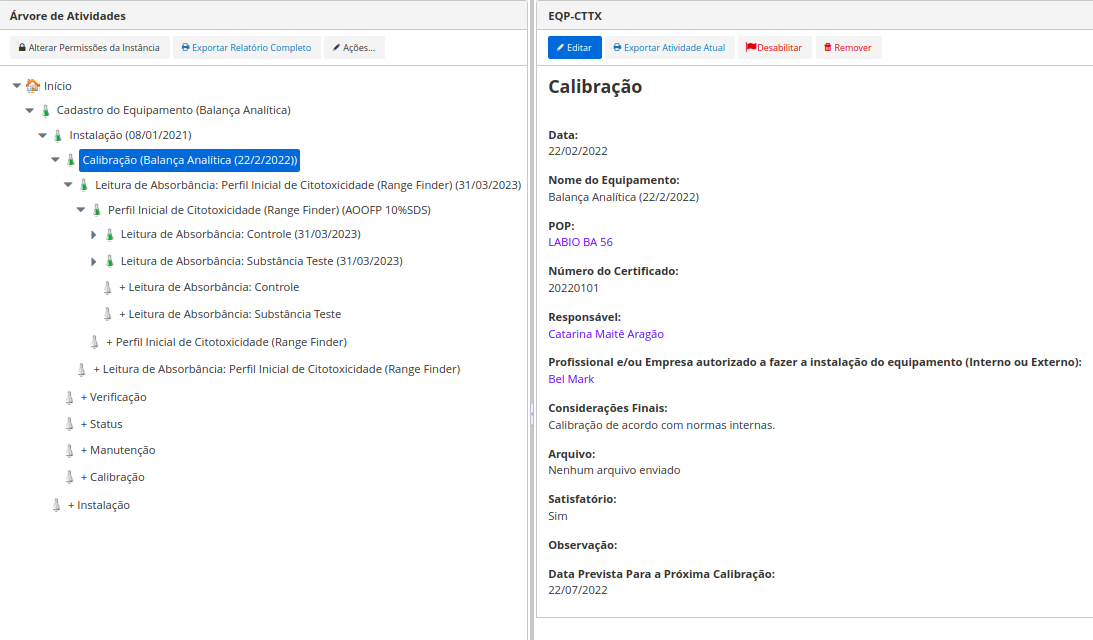
\includegraphics[width=0.7\textwidth]{imgs/CTTX-EQP/cttx_executado_calibracao_equipamento.png}
    \caption{Atividade de calibração executada seguindo o workflow de cadastro de equipamento, seguindo o cadastro e a instalação do mesmo. Podemos ver que a atividade de calibração é a mesma da figura~\ref{fig:cttx_executado_calibracao_leitura_absorbancia}}
    \label{fig:cttx_executado_calibracao_equipamento}
\end{figure}

\begin{figure}
    \centering
    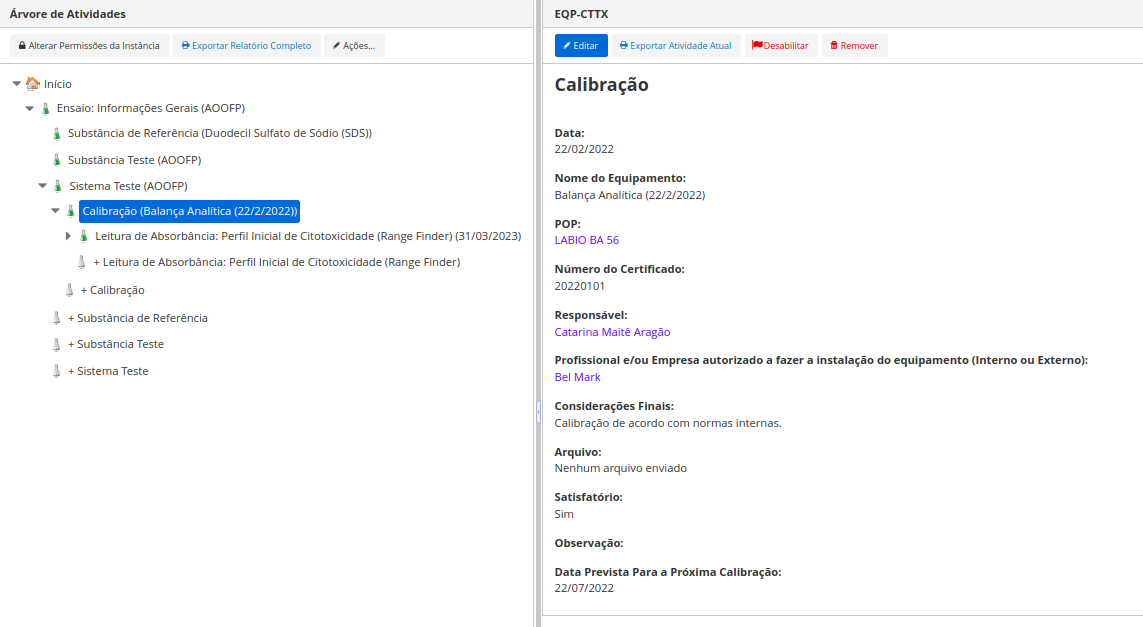
\includegraphics[width=0.7\textwidth]{imgs/CTTX-EQP/cttx_executado_calibracao_ensaio.png}
    \caption{Atividade de calibração executada seguindo o workflow de ensaio, que analisa as amostras. Podemos ver que a atividade de calibração é a mesma da figura~\ref{fig:cttx_executado_calibracao_equipamento}}
    \label{fig:cttx_executado_calibracao_leitura_absorbancia}
\end{figure}
% \subsection{Possível utilização em outros sistemas}

A utilização das funcionalidades citadas neste trabalho necessitam de um LIMS altamente personalizável para que a troca de ordem das atividades o processo de negócios feito. Além disso, deve ser possível modelar um workflow utilizando notação BPM para que seja utilizado a modelagem dentro do sistema.

Para que isso seja implementado de forma correta, o LIMS deve conseguir implementar a reordenação da modelagem de forma a centralizar a visualização atual em uma atividade, disponibilizando todas as outras atividades para manter as informações disponíveis.

O compartilhamento de atividades exige a existência de instâncias para cada execução do modelo criado. Isso ocorre porque o compartilhamento de informações deve ser feito para execuções específicas de um workflow (para uma equipamento específico cadastrado, por exemplo).

% Alterações feitas no BPM para que a feature possa ser utilizada em outros sistemas
\section{Conclusão}

Este trabalho apresenta uma implementação com novas funcionalidades focadas em melhorar a comunicação entre fluxos de trabalho e obtenção de dados de maneira rápida e eficiente dentro de LIMS que utilizam BPM: Workflows dinâmicos e compartilhamento de atividades entre workflows. Anteriormente, o sistema só poderia seguir a ordem das atividades como modelado inicialmente. Agora os workflows podem ser alterados para que a visualização seja relevante para o usuário que o está utilizando.

O compartilhamento de mensagens entre workflows também acelerou o acesso a informações entre times diferentes dentro de um mesmo laboratório que utiliza o LIMS. Atividades podem ficar dependentes de um outro fluxo de trabalho (conserto de equipamento, por exemplo) e a execução do mesmo pelo outro time de usuários disponibiliza novas atividades. Isso ajuda a diminuir a quantidade de erros que pode ocorrer no sistema e melhora a integração do laboratório às regras regulamentadoras que podem existir para determinado workflow.

Os workflows dinâmicos permitem que os usuários tenham uma interação completamente personalizada para o momento em questão, mudando a modelagem BPM de forma a encontrar informações e executar os seus trabalhos de maneira muito mais rápida e eficiente, alterando a interface do LIMS para que uma atividade em específica do workflow seja focada.
Essa centralização em uma atividade selecionada resulta em maior eficiência e flexibilidade no gerenciamento do projeto, facilitando o uso do software LIMS tanto para gerentes de laboratório quanto para técnicos.

A combinação de múltiplos workflows para pertencerem ao mesmo modelo BPM e compartilhar atividades possibilita que times diferentes dentro de um mesmo laboratório troquem informações entre si, permitindo o envio de notificações quando uma atividade for concluída, ou realizar o pedido de aprovação de uma atividade a um supervisor. Um médico pode fazer um pedido de exame ao laboratório do hospital, executando a atividade que notificará ao técnico de laboratório. O técnico irá aprovar ou reprovar a atividade, fazer todos os passos necessários e apenas o resultado do pedido de exame irá ser disponibilizado ao médico, tendo dois workflows unidos trocando informações entre diferentes usuários.

Este tipo de integração também pode ser utilizada com a implementação de workflows dinâmicos, deixando as implementações ainda mais eficientes. O compartilhamento de atividades dentro de um workflow facilita a acessibilidade de gerentes de laboratório às atividades de todo o processo que ocorre dentro da organização, dando a habilidade de alterar a visualização como um todo, remontando até os workflows unidos pela atividade compartilhada.

Essas implementações podem ser utilizadas em todos os workflows. Os workflows dinâmicos podem ser utilizados em modelos já implementados sem nenhuma alteração, mas levar em consideração que as atividades podem ser centralizadas pode ajudar na modelagem do BPM.

O compartilhamento de atividades pode ser implementado em novos workflows ou com adaptação de workflows já existentes, devendo ser remodelado para que haja a comunicação entre diferentes usuários do LIMS.

Foram realizados testes nos workflows BPL, CTTX e CENTRARE. Para os workflows BPL e CTTX, foi utilizada a implementação de compartilhamento de atividades, unindo múltiplos workflows e compartilhando informações entre eles. Para a implementação de workflows dinâmicos, foi utilizado o workflow CENTRARE pela sua complexidade e quantidade de atividades que devem ser executadas por diferentes usuários.

Foi feito com sucesso a implementação da funcionalidade no sistema LIMS Flux, que utiliza como base de montagem de workflows o Business Process Model (BPM), permitindo que administradores do Flux montassem workflows já com estas funcionalidades em mente para disponibilização de informações ao usuário, e também permitindo que usuários de workflows do Flux obtivessem informações com muito mais velocidade, aumentando a eficiência dos trabalhos realizados.

Como o sistema Flux utiliza de instâncias para separações dos workflows por execução, o compartilhamento de informações entre atividades foi feito para diferentes instâncias, ou seja, BPMs com construções diferentes podem comunicar entre execuções específicas de um workflow, ligando suas atividades onde necessário e, com isso, obtendo a funcionalidade de comunicação assíncrona entre usuários do sistema executando atividades que ficam disponíveis para outros.

Com isso, podemos unificar diferentes tipos de workflow utilizados em uma organização em um único workflow com múltiplas atividades iniciais. Assim, o workflow fica mais acessível para diferentes funcionários como gestor de laboratório, podendo ele acessar qualquer parte dos múltiplos workflows agrupados que fazem parte do laboratório e fazer a coleta e análise dos dados inseridos por outros funcionários, tudo em uma mesma tela.

A funcionalidade de workflows dinâmicos também funciona com a troca de informações, disponibilizando todas as informações de todas as instâncias compartilhadas quando a ordem das atividades é alterada, alterando o BPM para que o foco da execução atual seja na atividade selecionada.

Seguindo a utilização do Flux e a melhoria que obtivemos com workflows dinâmicos alterando a interface do usuário para que ela seja mais intuitiva e eficiente, temos que os resultados obtidos através de avaliação empírica foram muito positivos e que plataformas que implementam LIMS com BPM podem se beneficiar muito com este tipo de implementação. Para validar que haverá uma melhoria de eficiência quando implementado em um ambiente laboratorial real, é necessário fazer análises na velocidade de execução dos usuários.

Hoje o Flux já salva variáveis de horário de execução e acesso dos usuários às atividades, que poderiam ser utilizados para realizar um estudo estatística na velocidade dos trabalhos na utilização do sistema antes do recuso ser implementando e depois, fazendo a comparação de velocidade na execução dos trabalhos dos usuários que o utilizam.

Ainda existem problemas a serem atacados a partir deste trabalho, como a alteração da interface para melhor a identificação de pais diretos da atividade trocada e informações sobre compartilhamento de atividades, como quando atividades podem ser compartilhadas entre instâncias de mesmo tipo (hoje isso não é permitido: Pedidos de exame não são compartilhados entre laboratórios).

A árvore de atividades anteriores à atividade focada atualmente é necessária para garantir que todas as informações estejam disponíveis para execução de atividades futuras, mas quais atividades podem ser ofuscadas para garantir uma interface mais limpa e intuitiva pode ser estudado, já que não é possível saber quais informações serão importantes em um BPM genérico.

Além disso, é necessário realizar um estudo mais aprofundado sobre o compartilhamento de atividades com instâncias específicas, a fim de compreender de maneira abrangente com quais instâncias uma atividade pode ser compartilhada. Dessa forma, será possível determinar se as atividades podem ser compartilhadas com instâncias do mesmo tipo ou se a atividade deve conter propriedades que indiquem quais instâncias podem receber a informação, em vez de deixar essa escolha a critério do usuário. Essa análise detalhada tem o objetivo de automatizar o processo e torná-lo mais eficiente.

\bibliographystyle{unsrt}
% \addbibresource{bibliografia.bib}
% \bibliography{bibliografia}
\bibliography{mendeley}

% \nocite{*}

\end{document}

% Organização:
%   Intro: falar de sistemas biomédicos; 
%          falar de lims; 
%          falar de bpms; 
%          falar de lims baseados em bpms; 
%          falar dos problemas; 
%          falar da solução
%  Sistemas Biomédicos e LIMS
%         falar da importância
%         falar de lims
%         exemplos de sistemas - serve para motivar o trabalho
%  LIMS baseados em workflows
%         Flux
%         Problemas com atividades profundas
%  Workflows Dinâmicos
%         Para resolver este problema propomos...
%         Ilustrar o problema
%         Descrever a solução
%  Exemplos de Aplicações
%  Conclusão
 
        